\documentclass[lang=cn,10pt,device=pad]{elegantbook}
%titlestyle=display
%toc=twocol
\title{《拓扑学》学习笔记}
\subtitle{Practice makes perfect.}
%($\subset my$的)

%额外宏包
\usepackage{makeidx}
\makeindex
\usepackage{standalone}
\usepackage{pgfplotstable}
\usepackage{pgfplots}
\pgfplotsset{compat = newest}

%字体部分
\setCJKmainfont[ItalicFont=FandolKai-Regular,BoldFont=STSongti-SC-Black]{STSong} 
\setCJKsansfont{FandolHei-Regular}
\setCJKmonofont{FandolFang-Regular}
\setCJKfamilyfont{kaiti}{FandolKai-Regular}
\setCJKfamilyfont{cuk}{STKaitiSC-Black}
\setCJKfamilyfont{cusong}{STSongti-SC-Black}
\setCJKfamilyfont{fang}{FandolFang-Regular}
\newcommand{\kaiti}{\CJKfamily{kaiti}}%\
\newcommand{\cukaii}{\CJKfamily{cuk}}%\
\newcommand{\cusong}{\CJKfamily{cusong}}%\
\newcommand{\fang}{\CJKfamily{fang}}%
\usepackage{calligra}
\everymath{\displaystyle} 

\author{张博涵}
\institute{张博涵}
\date{起著重庄赤奋若}
\version{\today}
%\version{1.0}
\bioinfo{Github地址}{\href{www.github.com/BHanZhang}{www.github.com/BHanZhang}}

\extrainfo{摄于2022年07月28日~河南省~洛阳市~~{\calligra with}~{\calligra my}~{\calligra my}}

\setcounter{tocdepth}{3}

%\logo{logo-blue.png}
\cover{cover.jpg}

% 本文档命令
\definecolor{mygrn}{RGB}{21,153,65}
\definecolor{myor}{RGB}{252,113,21}
\definecolor{myblu}{RGB}{46,90,168}
%\renewcommand{\exists}{\exists~}
\usepackage{array}
\newcommand{\ccr}[1]{\makecell{{\color{#1}\rule{1cm}{1cm}}}}
\newcommand{\tl}[1]{\textcolor{myor}{#1}}
\newcommand{\gn}[1]{~\textcolor{mygrn}{\cusong{#1}}~}
\newcommand{\lei}[1]{~\textcolor{myblu}{\cusong{#1}}~}
\newcommand{\lanse}[1]{~\textcolor{myblu}{#1}~}
\newcommand{\tp}{\mathscr{F}}
\newcommand{\tpj}{\mathcal{B}}
\newcommand{\mj}[1]{\mathscr{P} (#1) }
\newcommand{\st}{~s.t.~}
\newcommand{\dabing}{\displaystyle\bigcup}
\newcommand{\dajiao}{\displaystyle\bigcap}
\newcommand{\dkh}[1]{\{#1\}}
\newcommand{\xkh}[1]{\left(#1\right)}
\newcommand{\chadiao}{\backslash}
\newcommand{\ranhou}{\Longrightarrow}
\newcommand{\cukai}[1]{{\cukaii{#1}}}
\newcommand{\R}{\mathbb{R}}
\newcommand{\hanshu}[1]{\left\{ \begin{aligned}
					#1
					\end{aligned} \right.}

% 重新定义
%\renewcommand{\exists}{\exists~}
% 修改标题页的橙色带
\definecolor{customcolor}{RGB}{249,125,28}
\colorlet{coverlinecolor}{customcolor}

% 图片并排
\usepackage{paracol}
\columnratio{0.5}           % 栏宽比例
%\setlength{\columnsep}{0em} 
%\setlength{\parskip}{.5ex plus 1pt}
\normalcolseprulecolor[black]
\setlength{\columnseprule}{0.4pt}
\newcommand{\zhu}[1]{\end{paracol}
\begin{paracol}{2}
\switchcolumn
#1
\vfill
\switchcolumn
}

\begin{document}

\maketitle
\frontmatter

\tableofcontents

\mainmatter
%第一部分
\part{点集拓扑}
%第一章
\chapter{拓扑空间}
\section{拓扑空间,开集}
\begin{definition}[拓扑空间,开集]\label{c1-d1}\index{拓扑空间}
	设$X$为一个集合$\mathscr{F}\in \mathscr{P}(X)$(把$\mathscr{F}$中的元素称为$X$中的\gn{开集}),满足:
	\begin{enumerate}
		\item $\emptyset , X \in \mathscr{F}$
		\item $U , V$是开集,那么$U\cap V$是开集
		\item $U_{\alpha} , \alpha\in I $是开集,$\dabing_{\alpha\in I}U_{\alpha}$是开集。
	\end{enumerate}
	则称$\mathscr{F}$为$X$上的一个\gn{拓扑},$(X,\tp)$为一个\gn{拓扑空间}。
\end{definition}

\begin{note}
	有时候这样写:“设$X$为拓扑空间”,这就意味着“$X$为一个集合,且规定了$X$上的一个拓扑(指定了那些子集为开集)”。
\end{note}


\begin{note}
	这里第二点可以更换为“有限个开集的交仍为开集”,这样的定义也与我们熟知的开集的性质相一致。
\end{note}
\begin{example}[欧氏拓扑]
	对于$n$维欧氏空间$\mathbb{R}^{n}$,$\tp  = \{\mathbb{R}^{n} \text{在通常意义下的开集} , \emptyset\}$构成一个拓扑空间。
\end{example}
\begin{proof}
	验证其为拓扑空间,就是要验证三条:
	
	\begin{enumerate}
		\item 第一条显然成立 : $\emptyset , \mathbb{R}^{n} \in \mathscr{F}$;
		\item 设$U,V$为$\mathbb{R}^{n}$中开集,要证$U\cap V$为开集。任取$x_{0}\in U\cap V$,就有:
		\begin{enumerate}
			\item $x_{0}\in U$ ,有$\exists \delta_{1} , \st   x_{0}\in B(x_{0},\delta_{1})\subset U$ 
			\item $x_{0}\in V$ ,有$\exists \delta_{2} , \st  x_{0}\in B(x_{0},\delta_{2})\subset V$ 
		\end{enumerate}
		择$\delta \in \min(\delta_{1},\delta_{2})$,有$x_{0}\in B(x_{0},\delta)\subset U\cap V$,那么$U\cap V$是开集;
		\item 任取$x_{0}\in \dabing_{\alpha \in  I} U_{\alpha}$,则必$\exists \alpha_{0}\in I \st x_{0} \in  U_{\alpha_{0}} $,则$\exists \delta \st x_{0}\in B(x_{0},\delta)\subset U_{\alpha_{0}}\subset \dabing_{\alpha \in  I} U_{\alpha}$ ,于是$\dabing_{\alpha \in  I} U_{\alpha}$是开集。
	\end{enumerate}
\end{proof}
\begin{example}[平凡拓扑]
	设$X$是一个集合,$\tp  = \{\emptyset,X \}$,则$\tp$显然是$X$上一个拓扑,称之为\gn{平凡拓扑}。
\end{example}
\begin{example}[离散拓扑]
	设$X$是一个集合,$\tp  = \mj{X} $,则$\tp$显然是$X$上一个拓扑,称之为\gn{离散拓扑}。
\end{example}
\begin{note}
以上两个例子说明,对于同一个集合,我们可以定义不同的拓扑,拓扑并不是唯一的,可以证明,平凡拓扑是$X$上最弱的拓扑,离散拓扑是$X$上最强的拓扑\footnote{如果$X,Y$是$T$上的两个拓扑,且$X\subset Y$那么就称拓扑$X$\gn{弱}于拓扑$Y$,反之拓扑$Y$\gn{强}于拓扑$X$。}	。

通过以后的学习可以知道,平凡拓扑具有较为“刚性”的拓扑结构,而离散拓扑具有较为“柔性”的拓扑结构。
\end{note}

\begin{definition}[度量空间]
	设$X$为一个集合,$\rho : X\times X\to \mathbb{R}$满足以下三条:
\begin{enumerate}
	\item $\rho(x,y) = \rho(y,x) $;
	\item $\rho(x,y)\geq 0 , \forall x,y \in X , \rho(x,y) = 0 \iff x = y$;
	\item $\rho(x,y)\leq\rho(x,z)+\rho(z,y) , \forall x,y,z\in X$
\end{enumerate} 	
那么就称$X,\rho$为一个\gn{度量空间},$\rho$为$X$上的一个\gn{度量}。
\end{definition}
\begin{example}[度量空间诱导的拓扑]
 设$(X,\rho)$为一个度量空间,定义$X$上开集$U$为:
	\begin{equation*}
		x_{0}\in U \iff \forall x_{0}\in U , \exists \delta >0,\st B(x_{0},\delta)\subset U
	\end{equation*}
	定义拓扑$\tp  = \mj{X}$,则$\tp$给出了$X$上的一个拓扑(称之为\gn{度量$\rho$诱导的拓扑})。
\end{example}
\begin{note}
这个例子说明了度量可以诱导拓扑,“赋范出度量,天然诱拓扑”。	
\end{note}

\begin{example}[$\mathbb{R}$上连续函数空间上的连续度量诱导的拓扑]
	定义$X = C([a,b])$上的连续度量$\rho$:
	\begin{equation*}
	\begin{aligned}
		\rho : C([a,b]) \times C([a,b])&\longrightarrow \mathbb{R}\\
		(f,g) &\longmapsto\rho(f,g):=\max_{x\in [a,b]}|f(x)-g(x)|
	\end{aligned}
	\end{equation*}
	此时$\rho$诱导了$C([a,b])$上的一个拓扑。
\end{example}
\begin{example}[除了“最大”和“最小”的拓扑之外,还存在“适中”的拓扑]
	设$X = \{0,1 \}$,$\tp =\{\emptyset , \dkh{0},\dkh{0,1}\}$是一个拓扑,$(X,\tp)$是一个拓扑空间。
\end{example}
\section{更多的拓扑空间与子空间拓扑}
\begin{definition}[子空间拓扑]
	设$X$是一个拓扑空间,$Y\subset X$为$X$的一个子集,则$Y$上可以如下定义一个拓扑结构:
	\begin{equation*}
		\tp =\dkh{U\cap Y| U\subset_{open} X}
	\end{equation*}
	则$\tp $定义了$Y$上的一个拓扑空间结构,此结构成为$X$在$Y$上诱导的拓扑,或称$Y$被赋予\gn{子空间拓扑}。
\end{definition}
\begin{proof}
	取大集合为小集合即可,证明显然。
\end{proof}
\begin{example}[$n$维单位球面]
$n$维单位球面$S^{n}\subset \mathbb{R}^{n}$赋予欧氏拓扑,其中$S^{n} = \dkh{x\in \mathbb{R}^{n}|~||x|| = 1}$。
\end{example}
\begin{example}[谈开集一定要说是在哪个拓扑的意义下是开集]
设$[0,1)\subset \mathbb{R}$,赋予$[0,1)$子空间拓扑,因为$(-\dfrac{1}{2},\dfrac{1}{2})$是$\mathbb{R}$中开集,$(\dfrac{1}{2},1)$也是$\mathbb{R}$中开集,那么有以下结论成立:
\begin{itemize}
	\item $[0,\dfrac{1}{2}):=(-\dfrac{1}{2},\dfrac{1}{2})\cap [0,1)$是开集。
	\item $(\dfrac{1}{2},1):=(\dfrac{1}{2},1)\cap [0,1)$是开集。
\end{itemize}

正如我们在$\mathbb{R}$中所规定的那样,上述两个例子分别应该不为开集和为开集,但是在子空间拓扑的意义下均为开集。这就说明了谈开集一定要说在哪个拓扑的意义下是开集。
\end{example}

\begin{definition}[连续性]
	若$f$是拓扑空间$X\longrightarrow Y$的映射,如果$\forall ~U\subset_{open} Y , f^{-1}(U)$为$X$中开集,则称映射$f$是\gn{连续的}。即连续映射到达域原像为开集。
\end{definition}

\begin{example}[离散拓扑为原像集的映射一定是连续映射]
	设$X$为一个集合,$\tp = \mj{X}$,是$X$上的离散拓扑,
	
	假设$f:X\longrightarrow Y$,那么对于$\forall U\subset_{open} Y , f^{-1}(U)\subset X$而$X$的所有子集都是开集(因为$X$的拓扑$\tp$是离散拓扑)。因此我们得知:\textbf{$X$上的任意映射都是连续的}。  
\end{example}

\begin{example}[平凡拓扑上的连续映射只能到平凡拓扑]
	设$X$为一个集合,$\tp = \dkh{\emptyset,X}$,是$X$上的平凡拓扑,
	
	设$Y$为一个拓扑空间,$f:X \longrightarrow Y$为一个连续映射,$f(X):=\dkh{f(x)|x\in X}\subset Y$(此处$f(X)$作为子空间赋予子空间拓扑),则$f:X \longrightarrow f(X)$仍是连续映射。下断言:\textbf{$f(X)$在子空间拓扑下只能为平凡拓扑空间}。
	
	假设$f(X)$不是平凡拓扑空间,那么\footnote{这里符号$\sqsubset$表示真被包含。}$\exists U\sqsubset f(X)$,并且$U\neq \emptyset$且为$f(X)$中开集,即$f^{-1}(U)\subset_{open}X$。
	
	但是$X$中开集只有两种可能,即$X$和$\emptyset$,因为$f:X \longrightarrow f(X)$是满射,因此$U$中的任何一点都有原像(但是原像不一定唯一),因此$f^{-1}(U)\neq \emptyset$。因此$f^{-1}(U) = X$。因此$f(X)=U  \sqsubset f(X)$相矛盾,因此:若$f:X \longrightarrow Y$是连续映射,则$f(X)$一定为平凡拓扑空间。
\end{example}

\section{开集的反面,闭集}
\begin{definition}[闭集]
	设$X$是拓扑空间,$F\subset X$,如果$X\backslash F $是$X$中开集,则$F$称为$X$中的\gn{闭集}。
\end{definition}
根据开集的性质(定义\ref{c1-d1})可立马得到闭集的性质:
\begin{proposition}[闭集的性质]
	\begin{enumerate}
		\item $\emptyset , X $是闭集
		\item $F ,G$是闭集,那么$ F \cup F$是闭集
		\item $F_{\alpha} , \alpha\in I $是开集,$\dajiao_{\alpha\in I}F_{\alpha}$是闭集。
	\end{enumerate}
\end{proposition}
\subsection{闭集之刻画}
\begin{definition}[极限点]
	设$X$是一个拓扑空间,$A\subset X$,$\forall p\in X$,若$\forall $包含$p$的开集$U$都有:
	\begin{equation*}
		(U\chadiao \dkh{p})\cap A \neq \emptyset
	\end{equation*}
	则称$p$为$A$的一个\gn{极限点}。而将集合$\overline{A} = A \cup \dkh{A\text{的极限点}}$称为$A$的\gn{闭包}。
\end{definition}
\begin{example}[欧氏空间中有理点的极限点集为欧氏空间]
	$X = \mathbb{R}^{3}$,$A$是$X$中的有理点(即$A\in \dkh{(x,y,z)|x,y,z\in \mathbb{Q}}$),那么$X$就是$A$的极限点集。
\end{example}
\begin{example}[欧氏空间中整数点的极限点集为空集]
	$X = \mathbb{R}^{3}$,$A=\mathbb{Z}$,那么$A$的极限点集为$\emptyset$。
\end{example}
\begin{example}[点集的极限点]
\label{c1-l13}
	设$X=\dkh{0,1}$,$\tp =\dkh{\dkh{0},\dkh{0,1},\emptyset}$则$X$的子集$A$有以下两种情况:
	\begin{enumerate}
		\item \lei{$A=\dkh{0}$:}
		\begin{enumerate}
			\item[\lei{0}]:$\forall $包含$\dkh{0}$的开集$U$,$(U\chadiao\dkh{0})\cap A = \emptyset$,说明0不是$A$的极限点。
			\item[\lei{1}]:$\forall $包含$\dkh{1}$的开集$U= \dkh{0,1}$(只有这一个),$(U\chadiao\dkh{1})\cap A \neq \emptyset$,说明1是$A$的极限点。
		\end{enumerate}
		因此1为$A = \dkh{0} $的极限点。
		\item \lei{$A=\dkh{1}$:}
		\begin{enumerate}
			\item[\lei{0}]:取包含$\dkh{0}$的开集$U = \dkh{0}$,$(U\chadiao\dkh{0})\cap A = \emptyset$,说明0不是$A$的极限点。
			\item[\lei{1}]:包含$\dkh{1}$的$X$中开集$U= \dkh{0,1}$,$(U\chadiao\dkh{1})\cap A = \emptyset$,说明1也不是$A$的极限点。
		\end{enumerate}
	\end{enumerate}
\end{example}
\begin{proposition}[闭集的等价刻画]
\label{c1-m2}
	设$X$为拓扑空间,$A\subset X$则:
	\begin{equation*}
		A\text{是闭集}\iff \overline{A} = A
	\end{equation*}
\end{proposition}
\begin{proof}[$\Rightarrow$]设$A$是闭集,要证$\overline{A} = A$,显然$A \subset\overline{A}$,下只需证$\overline{A} \subset A$,即证$X\chadiao A\subset X\chadiao\overline{A}$,因此对于$p\in X\chadiao A$都有$p\in X\chadiao\overline{A}$,因此即证:$\forall p \notin A$,$p$不是$A$的极限点。

事实上,$A$闭集$\Rightarrow X\chadiao A$开集$\iff  \exists$开集$U\subset A\chadiao A , p\in U \Rightarrow (U\chadiao\dkh{p})\cap A =\emptyset \Rightarrow p$不是$A$的极限点。

  
	[$\Leftarrow$]设$\overline{A} = A$,要证$A$是闭集。只要证$X\chadiao A$是开集,即:
	\begin{equation*}
		\forall p\in X\chadiao A , \exists \text{开集}U , \st p\in U\subset X\chadiao A
	\end{equation*}
	由于$p\notin A\Rightarrow p\notin \overline{A}$,则$p$不为$A$的极限点。
	因此$\exists $开集$U\subset X(p\in U) \st (U)\cap A = (U\chadiao \dkh{p})\cap A = \emptyset $,即$p\in U\subset X\chadiao A$
\end{proof}
\begin{corollary}
	\begin{center}
		$\overline{A}$为一个闭集。
	\end{center}
\end{corollary}
\begin{proof}
	只要证$X\chadiao \overline{A}$为开集。 由于
$
		\forall p \in X\chadiao \overline{A} ,  p\text{不为}A\text{的极限点}
$则$\exists$开集$U\subset X \st p\in U$且由于$p\notin A$则$U\cap A = (U\chadiao \dkh{p}) \cap A  = \emptyset$

则$p\in U\subset X\chadiao A$

则$\forall q\in U$,$U$为包含$q$的开集,又由于$U\cap A =\emptyset$ ,因此$q$不是$A$的极限点,所以$q\notin \overline{A}$,故$U\subset X\chadiao \overline{A}$。

因此$X\chadiao\overline{A}$为开集。
\end{proof}
\begin{corollary}
	\begin{equation*}
		\overline{A} = \bigcap_{F\supset_{closed}A} F
	\end{equation*}
\end{corollary}
	
	\begin{note}
	由上推论可以知道,任何一个包含$A$的闭集都包含$\overline{A}$,而根据$\overline{A} = A \cup \dkh{A\text{的所有极限点}}$。因此$\overline{A}$为包含$A$的最小的闭集。	
	\end{note}

\begin{proof}
	[$\supset$]:由于$\overline{A}\supset_{closed}A$,那么必然可以取到$F_{0} =_{closed} \overline{A}$,此时$\dajiao_{F\supset_{closed}A} F = F_{0}\cap\xkh{\dajiao_{F_{0} \neq F\supset_{closed}A} F}\subset A$。
	
	
	[$\subset$]:只要证$\forall F\supset_{closed} A$都有$F\supset \overline{A}$,即证$X\chadiao F\subset X\chadiao \overline{A}$。
	
	只要证$\forall x \notin F , x$不为$A$的极限点。
	
	事实上,$F$是闭集,根据命题\ref{c1-m2}可知$F =\overline{F} \Rightarrow x\notin \overline{F}$,因此$x$不为$F$的极限点,而$F\supset{A}$因此得证。
\end{proof}

\begin{proposition}[闭包运算的性质]
	\begin{enumerate}
		\item $\overline{A\cup B} = \overline{A}\cup \overline{B}$
		\item $\overline{A\cap B} \subset \overline{A}\cap \overline{B}$ 
	\end{enumerate}
\end{proposition}
\begin{proof}
	额,不知道什么高级方法,于是采用土办法就好了。
	\begin{enumerate}
		\item  只需要证明$A\cup B$的极限点和$A$的极限点或$B$的极限点一致就好,事实上我们有如下的推理\footnote{这里会利用到集合运算的分配律 $A\cap (B\cup C) = (A\cap B)\cup(A\cap C)$和$A\cup (B\cap C) = (A\cup B)\cap(A\cup C)$}:
		\begin{equation*}
			\begin{aligned}
				x_{0}\text{是}A\cup B\text{的极限点}&\iff \forall x_{0}\in A\cup B , \exists_{open}V(x_{0}\in V) \st (V\chadiao\dkh{x_{0}})\cap (A\cup B)\neq \emptyset\\
				&\iff \xkh{(V\chadiao\dkh{x_{0}})\cap A}\cup \xkh{(V\chadiao\dkh{x_{0}})\cap B} \neq \emptyset\\
				&\iff \xkh{(V\chadiao\dkh{x_{0}})\cap A}\neq \emptyset~\text{或}~\xkh{(V\chadiao\dkh{x_{0}})\cap B}\neq \emptyset\\
				&\iff x_{0}\text{是}A\text{的极限点,或}B\text{的极限点}
			\end{aligned}
		\end{equation*}
		\item 只需要证明$A\cap B$的极限点就是$A$的极限点和$B$的极限点就好,事实上:
		\begin{equation*}
			\begin{aligned}
				x_{0}\text{是}A\cap B\text{的极限点}&\iff \forall x_{0}\in A\cap B , \exists_{open}V(x_{0}\in V) \st (V\chadiao\dkh{x_{0}})\cap (A\cap B)\neq \emptyset\\
				&\iff \xkh{(V\chadiao\dkh{x_{0}})\cap A}\cap \xkh{(V\chadiao\dkh{x_{0}})\cap B} \neq \emptyset\\
				&\Longrightarrow \xkh{(V\chadiao\dkh{x_{0}})\cap A}\neq \emptyset~\text{且}~\xkh{(V\chadiao\dkh{x_{0}})\cap B}\neq \emptyset\\
				&\iff x_{0}\text{是}A\text{的极限点,且是}B\text{的极限点}
			\end{aligned}
		\end{equation*}
	\end{enumerate}
	这一部分不是等号的问题主要出现在倒数第二步,因为两个非空集合的交不一定非空,而两个非空集合的并,一定非空。
\end{proof}
\begin{example}[上命题第二部分不能取等]
若$A = [0,1) , B = (1,2]$那么	$\overline{A\cap B}  = \emptyset \sqsubset  \dkh{1} = \overline{A}\cap \overline{B}  $
\end{example}
\begin{example}[单点集不一定是闭集,稠密]
	设$X=\dkh{0,1}$,$\tp =\dkh{\dkh{0},\dkh{0,1},\emptyset}$,于是拓扑空间的闭集就是直接取$\tp$在$X$中的补集,即$\dkh{\dkh{1},\emptyset,\dkh{0,1}}$,对比之后明显可以看出来$A = \dkh{0}$不是闭集(其他几个都是既开又闭)。根据我们前面例\ref{c1-l13}的经验,$\dkh{0}$的极限点是$1$,因此$\overline{A} = A\cup \dkh{A\text{的极限点}} = \dkh{0,1} = X$。即取了闭包之后就取到全集,这种现象我们称之为\textbf{稠密}。
\end{example}
\subsection{稠密}
\begin{definition}[稠密]
	设$X$为一个拓扑空间,$A\subset X$,若$\overline{A} = X$则称$A$在$X$中\gn{稠密}。如果$Y\subset X$是$X$的拓扑子空间,如果还有$Y$的拓扑子空间$Z\subset Y$那么我们分别记:
	\begin{enumerate}
		\item[$\overline{Z_{Y}}$] :$Z$在$Y$中取闭包。
		\item[$\overline{Z_{X}}$] :$Z$在$X$中取闭包。
	\end{enumerate}
\end{definition}
\begin{note}
之所以会在不同背景集合中取闭包,最本质是因为某集合在不同背景集合中的极限点是不一样的。	
\end{note}

\begin{example}[同一集合在不同背景集合中取闭包不相一致]
	设$X =\mathbb{R} , Y  =(0,2) , Z=(0,1)$于是取闭包:$\overline{Z_{X}} = [0,1] , \overline{Z_{Y}} = (0,1]$	
\end{example}
\begin{example}[有理数集$\mathbb{Q}$在实数集$\mathbb{R}$中稠密]
	因为有理数集$\mathbb{Q}$的极限点集为实数集$\mathbb{R}$,因此$\overline{\mathbb{Q}} = \mathbb{R}$。
\end{example}

那么很自然就产生疑问,是否取闭包的运算和子空间拓扑存在很多联系?这就是下面命题所解决的:
\begin{proposition}
\label{c1-m4}
	设$X$是拓扑空间,$Y$是$X$的拓扑子空间,$Z$是$Y$的拓扑子空间。我们有:
	\begin{equation*}
		\overline{Z_{Y}} = \overline{Z_{X}} \cap Y
	\end{equation*}
\end{proposition}
\begin{proof}
	验证这一问题,仍然从土方法走:
	\begin{enumerate}
		\item[\lei{[$\subset$]}] 即证$\forall x\in \overline{Z_{Y}}, \st x\in \overline{Z_{X}} \cap Y$,首先因为$x\in \overline{Z_{Y}}$,因此$x\in Y$于是只需证$x\in \overline{Z_{Y}}$:
		\begin{enumerate}
			\item $x \in Z $显然成立
			\item $x \notin Z $,此时意味着$x$为$Z$在$Y$中的极限点,只需证$x\in \overline{Z_{X}}$,即证$x$为$Z$在$X$中的极限点。
			
			
			事实上$\forall x$在$X$中的开邻域$V$,有:对于$X$在$Y$中的去心开邻域\gn{$\xkh{(V\cap Y)\chadiao \dkh{x}}$}有:
			\begin{equation*}
				\begin{aligned}
					&\gn{\xkh{(V\cap Y)\chadiao \dkh{x}}}\cap Z\\
					=& \xkh{(V\chadiao \dkh{x})\cap Z}\cap Y\\
					\subset & \lei{(V\chadiao\dkh{x})\cap Z}\neq\emptyset\\
				\end{aligned}
			\end{equation*}
		\end{enumerate}
\begin{figure}[ht]
\centering
\tikzset{every picture/.style={line width=0.75pt}}
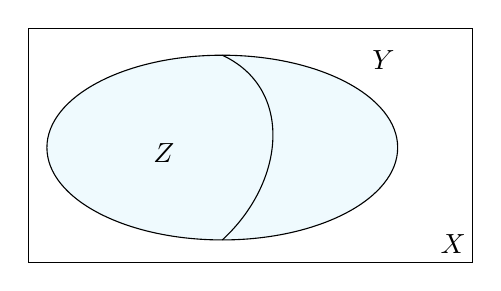
\begin{tikzpicture}[x=0.75pt,y=0.75pt,yscale=-1,xscale=1]
\draw   (100,57) -- (314,57) -- (314,170) -- (100,170) -- cycle ;
\draw  [fill={rgb, 255:red, 239; green, 250; blue, 254 }  ,fill opacity=1 ] (109,114.5) .. controls (109,89.92) and (146.83,70) .. (193.5,70) .. controls (240.17,70) and (278,89.92) .. (278,114.5) .. controls (278,139.08) and (240.17,159) .. (193.5,159) .. controls (146.83,159) and (109,139.08) .. (109,114.5) -- cycle ;
\draw    (193.5,70) .. controls (228,86) and (224,131) .. (193.5,159) ;
\draw (159,111.4) node [anchor=north west][inner sep=0.75pt]    {$Z$};
\draw (264.5,66.4) node [anchor=north west][inner sep=0.75pt]    {$Y$};
\draw (312,166.6) node [anchor=south east] [inner sep=0.75pt]    {$X$};
\end{tikzpicture}
\caption{命题1.4之集合关系图}
\end{figure}
		\item[\lei{[$\supset$]}] 即证$\forall x\in \overline{Z_{X}}\cap Y , \st x\in \overline{Z_{Y}}$,首先明显有$x\in Y$于是仍分类讨论:
		\begin{enumerate}
			\item $x\in Z$显然成立
			\item $x\notin Z$,此时意味着$x$为$Z$在$X$中的极限点,只需证$x\in \overline{Z_{X}}$,即证$x$为$Z$在$Y$中的极限点。
			
			事实上,任意在$Y$中的包含$x$的开集,由子空间拓扑,不妨设之为$V\cap Y$,其中$V\subset_{open} X (x\in V)$,因为$x$为$Z$在$X$中的极限点,所以$(V\chadiao\dkh{x})\cap Z \neq \emptyset$,又由于$x\in Y$,所以$(V\chadiao \dkh{x})\cap Z\cap Y = (V\cap(Y\chadiao\dkh{x}))\cap Z \neq \emptyset$   
		\end{enumerate}
	\end{enumerate}
\end{proof}
更进一步,我们问以下的问题:
\begin{problem}
	设$X$是拓扑空间,$F\subset X$稠密,$U\subset X$,问:$F\cap U$是否在$U$中稠密?
\end{problem}

答案是否定的,因为如果偷鸡取$U = X\chadiao F$这件事就算寄了。于是为了排除这个情况,我们必须要求$U$是开集。如下命题:
\begin{proposition}
		设$X$是拓扑空间,$F\subset X$稠密,$U\subset_{open} X$是$X$且赋予子空间拓扑,则$F\cap U$在$U$中稠密。
\end{proposition}
\begin{proof}
	要证$\overline{(F\cap U)_{U}} = U$根据命题\ref{c1-m4},即要证$\overline{(F\cap U)_{U}}\cap U = U$,即要证$U\subset \overline{(F\cap U)_{X}}$。
	
	即对$\forall x\in U$要证$x\in \overline{(F\cap U)_{X}}$。则分两类讨论:
	\begin{enumerate}
		\item $x\in F\cap U$ 显然成立
		\item $x\notin F\cap U$ ,又由于$F$在$X$中稠密,那么$x$是$F$的极限点,\tl{任取$X$中开集$V(x\in V)$},由于$U$是$X$中开集,因此$V\cap U$也是$X$中开集,因为$x$是$F$的极限点,所以有:
		\begin{equation*}
			\begin{aligned}
				&\xkh{(V\cap U)\chadiao \dkh{x}}\cap F \neq \emptyset\\
				\iff & \tl{(V\chadiao\dkh{x})\cap(F\cap U)\neq \emptyset}
			\end{aligned}
		\end{equation*}
	\end{enumerate}
\end{proof}
\begin{note}
这里做一个小小小的总结,一个开集的闭包是闭集,也就是说闭集包括了这个开集中的所有的元素和这个开集的全部极限点,因此在这个开集中取任何点列其极限点均在这个集合的闭包里(闭集也一样,闭集的闭包为其自己)。因此我们知道闭集中“闭”的含义是\cukai{闭集关于取极限运算是封闭的!}。	
\end{note}

\subsection{集合之解体}
为了更好说话,引入以下概念:
\begin{definition}[内点,外点,边界点]
设X为一个拓扑空间,$A\subset X$定义:
\begin{itemize}
	\item 定义$A$的\gn{内点集}:$int(A) : = \dkh{p\in A | \exists X\text{中开集}V(p\in V) , V\subset A}$
	\item 定义$A$的\gn{外点集}:$ext(A) : = \dkh{p\notin A | \exists X\text{中开集}V(p\in V) , V\subset X\chadiao A} \iff int(X\chadiao A)$ 
	\item 定义$A$的\gn{边界点集}:$\partial(A) := \dkh{p\in X | \forall p\text{的开邻域}V,V\cap A \neq \emptyset.V\cap(X\chadiao A) \neq \emptyset}$
\end{itemize}
\end{definition}
\begin{note}
根据以上定义,我们显然有:
\begin{equation*}
	X = int(A) \sqcup ext(A) \sqcup \partial(A)
\end{equation*}
\end{note}
\begin{example}[一些显然的例子]
	\begin{enumerate}
		\item 设$A = [0,1)\subset \mathbb{R}$那么:$\partial(A) = \dkh{0,1} , int(A) = \xkh{0,1} , ext(A) = (-\infty,0)\cup(1,+\infty)$
		\item \begin{enumerate}
		\item 设$A = (0,1)\subset [0,1)$那么:$\partial(A) = \dkh{0} , int(A) = \xkh{0,1} , ext(A) = \emptyset$
		\item 设$A = (0,1)\subset \mathbb{R}$那么:$\partial(A) = \dkh{0,1} , int(A) = \xkh{0,1} , ext(A) = (-\infty,0)\cup(1,+\infty)$
		\end{enumerate}
		\item 设$D = \dkh{(x,y)\in \mathbb{R}^{2}|x^{2}+y^{2}<1} $于是:\begin{enumerate}
		\item $\partial(D) = S^{1} =  \dkh{(x,y)\in \mathbb{R}^{2}|x^{2}+y^{2}=1}$
		\item $int(D) = D$
		\item $ext(D) =  \dkh{(x,y)\in \mathbb{R}^{2}|x^{2}+y^{2}>1}$
		\begin{figure}[h]
			\centering
\tikzset{every picture/.style={line width=0.75pt}}
\begin{tikzpicture}[x=0.75pt,y=0.75pt,yscale=-1,xscale=1]
\draw    (163,135) -- (320,135) ;
\draw [shift={(322,135)}, rotate = 180] [color={rgb, 255:red, 0; green, 0; blue, 0 }  ][line width=0.75]    (10.93,-3.29) .. controls (6.95,-1.4) and (3.31,-0.3) .. (0,0) .. controls (3.31,0.3) and (6.95,1.4) .. (10.93,3.29)   ;
\draw    (238.5,206) -- (238.5,51) ;
\draw [shift={(238.5,49)}, rotate = 90] [color={rgb, 255:red, 0; green, 0; blue, 0 }  ][line width=0.75]    (10.93,-3.29) .. controls (6.95,-1.4) and (3.31,-0.3) .. (0,0) .. controls (3.31,0.3) and (6.95,1.4) .. (10.93,3.29)   ;
\draw  [dash pattern={on 4.5pt off 4.5pt}] (194.25,135) .. controls (194.25,110.56) and (214.06,90.75) .. (238.5,90.75) .. controls (262.94,90.75) and (282.75,110.56) .. (282.75,135) .. controls (282.75,159.44) and (262.94,179.25) .. (238.5,179.25) .. controls (214.06,179.25) and (194.25,159.44) .. (194.25,135) -- cycle ;
\draw (324,138.4) node [anchor=north west][inner sep=0.75pt]    {$x$};
\draw (240.5,52.4) node [anchor=north west][inner sep=0.75pt]    {$y$};
\draw (284.75,138.4) node [anchor=north west][inner sep=0.75pt]    {$1$};
\draw (240.5,138.4) node [anchor=north west][inner sep=0.75pt]    {$0$};
\end{tikzpicture}
\caption{例1.18.3之拓扑空间$D$}
		\end{figure}
		\end{enumerate}
		\item 设$A = [0,1]\subset \mathbb{R}^{2}$,此时$\partial(A) = A , int(A) = \emptyset , ext(A) = X\chadiao A$
		\begin{figure}[h]
			\centering
\tikzset{every picture/.style={line width=0.75pt}}
\begin{tikzpicture}[x=0.75pt,y=0.75pt,yscale=-1,xscale=1]
\draw    (100,128) -- (261,128) ;
\draw [shift={(263,128)}, rotate = 180] [color={rgb, 255:red, 0; green, 0; blue, 0 }  ][line width=0.75]    (10.93,-3.29) .. controls (6.95,-1.4) and (3.31,-0.3) .. (0,0) .. controls (3.31,0.3) and (6.95,1.4) .. (10.93,3.29)   ;
\draw    (140,172) -- (140,86) ;
\draw [shift={(140,84)}, rotate = 90] [color={rgb, 255:red, 0; green, 0; blue, 0 }  ][line width=0.75]    (10.93,-3.29) .. controls (6.95,-1.4) and (3.31,-0.3) .. (0,0) .. controls (3.31,0.3) and (6.95,1.4) .. (10.93,3.29)   ;
\draw [color={rgb, 255:red, 208; green, 2; blue, 27 }  ,draw opacity=1 ]   (140,128) -- (176,128) ;\draw (142,131.4) node [anchor=north west][inner sep=0.75pt]    {$0$};
\draw (178,131.4) node [anchor=north west][inner sep=0.75pt]    {$1$};
\draw (265,131.4) node [anchor=north west][inner sep=0.75pt]    {$x$};
\draw (142,87.4) node [anchor=north west][inner sep=0.75pt]    {$y$};
\end{tikzpicture}
\caption{例1.18.4之拓扑空间$A$}
		\end{figure}
	\end{enumerate}
\end{example}
\section{拓扑空间的砖头---拓扑基}
\begin{definition}[拓扑基]\index{拓扑基}
	设$X$是拓扑空间,$\tpj$是一个由一些$X$中开集构成的集族,如果对$\forall X$中开集$U$,$U$均可表为$\tpj$中一些元素之并,则称$\tpj$构成了$X$的一个\gn{拓扑基}。
\end{definition}
\begin{example}[$\mathbb{R}^{1}$中的欧氏拓扑可以有不同的拓扑基]
\label{c1-e19}
	很明显,$\mathbb{R}^{1}$有一个拓扑基为$\tpj = \dkh{(a,b)|a<b}$。
	
	令$\tpj '  = \dkh{(a,b)|a<b,a,b\in \mathbb{Q}}$,则$\tpj ' $也是$\mathbb{R}^{1}$的一个拓扑基。
	\begin{proof}
		$\forall U\subset_{open} \mathbb{R}^{1},\forall p\in U$,则存在$a<p<b$使得$(a,b)\subset U$,从而由有理数集的稠密性可知,$\exists(a_{p},b_{p})\in \tpj',\st p\in (a_{p},b_{p})\subset U$即$U = \dajiao_{p\in U}(a_{p},b_{p})$。
		\begin{figure}[h]
			\centering
\tikzset{every picture/.style={line width=0.75pt}}
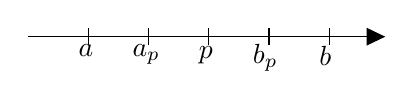
\begin{tikzpicture}[x=0.75pt,y=0.75pt,yscale=-1,xscale=1]
\draw    (100,101) -- (212,101) -- (227,101) -- (269,101) (129,97) -- (129,105)(158,97) -- (158,105)(187,97) -- (187,105)(216,97) -- (216,105)(245,97) -- (245,105) ;
\draw [shift={(272,101)}, rotate = 180] [fill={rgb, 255:red, 0; green, 0; blue, 0 }  ][line width=0.08]  [draw opacity=0] (8.93,-4.29) -- (0,0) -- (8.93,4.29) -- cycle    ;
\draw (181,104.4) node [anchor=north west][inner sep=0.75pt]    {$p$};
\draw (123,103.4) node [anchor=north west][inner sep=0.75pt]    {$a$};
\draw (239,104.4) node [anchor=north west][inner sep=0.75pt]    {$b$};
\draw (149,103.4) node [anchor=north west][inner sep=0.75pt]    {$a_{p}$};
\draw (207,103.4) node [anchor=north west][inner sep=0.75pt]    {$b_{p}$};
\end{tikzpicture}
\caption{例1.19之数轴}
		\end{figure}
	\end{proof}
\end{example}
\begin{note}
由此可见,一个拓扑空间可以有诸多拓扑基,但是一个拓扑基是否唯一确定一个拓扑空间呢?答案是肯定的,这个结论将由以下讨论给出。	
\end{note}

了解了定义,我们就需要探究一个拓扑基$\tpj$之所以为拓扑基的等价条件。很明显,由拓扑基我们可以知道拓扑基的必要条件,如下面这个命题:
\begin{proposition}
	设$X$为拓扑空间,$\tpj$为$X$的一个拓扑基,那么:
	\begin{enumerate}
		\item[\lei{TB1}]. $\dabing_{U\in \tpj}U = X$
		\item[\lei{TB2}]. $\forall U_{1},U_{2}\in \tpj \st U_{1}\cap U_{2}$可以表示为$\tpj$中一些元素之并。
	\end{enumerate}
\end{proposition}

\begin{proof}
	显然。
\end{proof}

这个命题反过来也是正确的,即有以下的命题:
\begin{proposition}
	设$X$为一个集合,$\tpj$为$X$的一个由一些子集构成的集族,若$\tpj$满足以上\lei{TB1}、\lei{TB2}两条,则$\tpj$必为$X$上某个拓扑$\tp$的拓扑基。而且,$\tp$是唯一的,称之为由拓扑基$\tpj$\gn{生成}的拓扑。
\end{proposition}
\begin{proof}
	定义$\tp=\dkh{\emptyset}\cup\dkh{\tpj\text{中若干元素之并}}=\dkh{\bigcup_{\alpha\in I}U_{\alpha}|U_{\alpha}\in \tpj}\cup\dkh{\emptyset}$,我们所要证明的是以下两点:
	\begin{enumerate}
		\item $\tp$是$X$上的一个拓扑。
	事实上,我们有:
	\begin{enumerate}
		\item $\emptyset , X\in \tp$(显然,由定义和条件\lei{TB1}可以保证。)
		\item $\tp$对于任意并封闭是显然的(因为就是这样定义的。)
		\item 对于$\forall \dabing_{\alpha \in I}U_{\alpha} , \dabing_{\beta\in J}V_{\beta}\in \tp$,其中$U_{\alpha},V_{\beta}\in \tpj,\forall \alpha \in I,\beta\in J$那么有:
		\begin{equation*}
			\xkh{\dabing_{\alpha\in I}U_{\alpha}}\cap\xkh{\dabing_{\beta\in J}V_{\beta}} = \dajiao_{\alpha,\beta}(U_{\alpha}\cap V_{\beta}) \in \tp
		\end{equation*}
	\end{enumerate}
	\item $\tpj$为拓扑$\tp$上的一个拓扑基。
	\end{enumerate}
	根据定义可知$\tpj$也确实为拓扑$\tp$上的一个拓扑基。从构造来看,我们并没有规定在拓扑基$\tpj$中的并是哪些,因此$\tp$是唯一的,因此命题得证。
\end{proof}
\begin{example}[$\mathbb{R}^{2}$的另一拓扑基]
	明显来看,欧氏空间$\mathbb{R}^{2}$中的开球的全体构成的集合是$\mathbb{R}^{2}$的一个拓扑基,根据我们在度量空间中所积攒的经验,$\mathbb{R}^{2}$中的开球和邻域是等价的,很自然的我们可以考虑$\mathbb{R}^{2}$中的开矩体的全体构成的集合$\tpj' = \dkh{(a,b)\times(c,d)|a<b,c<d}\cup\dkh{\emptyset}$:
	\begin{figure}[h]
		\centering
\tikzset{every picture/.style={line width=0.75pt}}
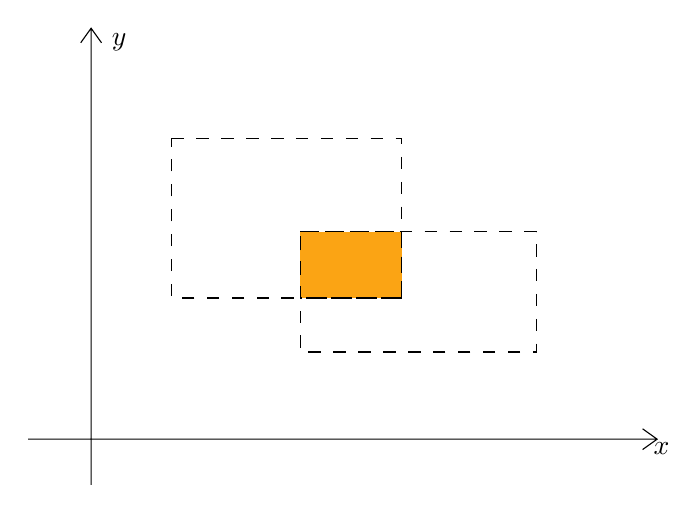
\begin{tikzpicture}[x=0.75pt,y=0.75pt,yscale=-1,xscale=1]
\draw  (43,229) -- (346,229)(73.3,31) -- (73.3,251) (339,224) -- (346,229) -- (339,234) (68.3,38) -- (73.3,31) -- (78.3,38)  ;
\draw  [fill={rgb, 255:red, 251; green, 164; blue, 20 }  ,fill opacity=1 ][dash pattern={on 4.5pt off 4.5pt}] (223,161) -- (174,161) -- (174,129) -- (223,129) -- (223,161) -- cycle ;
\draw  [dash pattern={on 4.5pt off 4.5pt}] (112,84) -- (223,84) -- (223,161) -- (112,161) -- cycle ;
\draw  [dash pattern={on 4.5pt off 4.5pt}] (174,129) -- (288,129) -- (288,187) -- (174,187) -- cycle ;
\draw (343,229.4) node [anchor=north west][inner sep=0.75pt]    {$x$};
\draw (82,32.4) node [anchor=north west][inner sep=0.75pt]    {$y$};
\end{tikzpicture}
\caption{例1.20之开矩体}
	\end{figure}
	
	很明显$\tpj'$是$\mathbb{R}^{2}$上某拓扑的拓扑基。
\end{example}
为了更好地描述两个拓扑基之间的关系,以便更加方便地研究两个拓扑基生成的拓扑空间之间的关系,我们对拓扑基引入如下的定义:
\begin{definition}[拓扑基之间的等价]
设$\tpj,\tpj'$满足\lei{TB1}、\lei{TB2},称$\tpj$与$\tpj'$是\gn{等价}的,若:
\begin{enumerate}
	\item $\forall U\in \tpj,p\in U,$都$\exists U'\in \tpj',\st p\in U'\subset U$
	\item $\forall V\in \tpj',p'\in V',$都$\exists V\in \tpj',\st p\in V\subset V'$
\end{enumerate}
\end{definition}

\begin{figure}[h]
\centering
 {
  \begin{minipage}{5cm}
   \centering
\tikzset{every picture/.style={line width=0.75pt}}
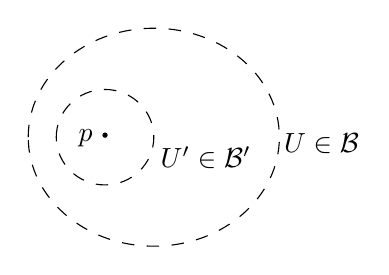
\begin{tikzpicture}[x=0.75pt,y=0.75pt,yscale=-1,xscale=1]
\draw  [dash pattern={on 4.5pt off 4.5pt}] (105,146.5) .. controls (105,117.51) and (132.09,94) .. (165.5,94) .. controls (198.91,94) and (226,117.51) .. (226,146.5) .. controls (226,175.49) and (198.91,199) .. (165.5,199) .. controls (132.09,199) and (105,175.49) .. (105,146.5) -- cycle ;
\draw  [dash pattern={on 4.5pt off 4.5pt}] (118.5,146.5) .. controls (118.5,133.8) and (129.02,123.5) .. (142,123.5) .. controls (154.98,123.5) and (165.5,133.8) .. (165.5,146.5) .. controls (165.5,159.2) and (154.98,169.5) .. (142,169.5) .. controls (129.02,169.5) and (118.5,159.2) .. (118.5,146.5) -- cycle ;
\draw  [fill={rgb, 255:red, 0; green, 0; blue, 0 }  ,fill opacity=1 ] (141,145.5) .. controls (141,144.95) and (141.45,144.5) .. (142,144.5) .. controls (142.55,144.5) and (143,144.95) .. (143,145.5) .. controls (143,146.05) and (142.55,146.5) .. (142,146.5) .. controls (141.45,146.5) and (141,146.05) .. (141,145.5) -- cycle ;
\draw (128,141.4) node [anchor=north west][inner sep=0.75pt]    {$p$};
\draw (167.5,149.9) node [anchor=north west][inner sep=0.75pt]    {$U'\in \tpj'$};
\draw (227,143.4) node [anchor=north west][inner sep=0.75pt]    {$U\in \tpj$};
\end{tikzpicture}
  \end{minipage}
 }
    {
     \begin{minipage}{6cm}
      \centering
      \tikzset{every picture/.style={line width=0.75pt}}
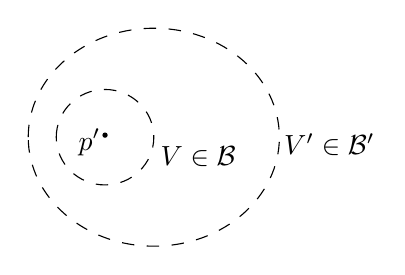
\begin{tikzpicture}[x=0.75pt,y=0.75pt,yscale=-1,xscale=1]
\draw  [dash pattern={on 4.5pt off 4.5pt}] (105,146.5) .. controls (105,117.51) and (132.09,94) .. (165.5,94) .. controls (198.91,94) and (226,117.51) .. (226,146.5) .. controls (226,175.49) and (198.91,199) .. (165.5,199) .. controls (132.09,199) and (105,175.49) .. (105,146.5) -- cycle ;
\draw  [dash pattern={on 4.5pt off 4.5pt}] (118.5,146.5) .. controls (118.5,133.8) and (129.02,123.5) .. (142,123.5) .. controls (154.98,123.5) and (165.5,133.8) .. (165.5,146.5) .. controls (165.5,159.2) and (154.98,169.5) .. (142,169.5) .. controls (129.02,169.5) and (118.5,159.2) .. (118.5,146.5) -- cycle ;
\draw  [fill={rgb, 255:red, 0; green, 0; blue, 0 }  ,fill opacity=1 ] (141,145.5) .. controls (141,144.95) and (141.45,144.5) .. (142,144.5) .. controls (142.55,144.5) and (143,144.95) .. (143,145.5) .. controls (143,146.05) and (142.55,146.5) .. (142,146.5) .. controls (141.45,146.5) and (141,146.05) .. (141,145.5) -- cycle ;
\draw (128,141.4) node [anchor=north west][inner sep=0.75pt]    {$p'$};
\draw (167.5,149.9) node [anchor=north west][inner sep=0.75pt]    {$V\in \tpj$};
\draw (227,143.4) node [anchor=north west][inner sep=0.75pt]    {$V'\in \tpj'$};
\end{tikzpicture}
     \end{minipage}
    }
		\caption{定义1.10之说明}
	\end{figure}
	
	\begin{proposition}
		设$\tpj$与$\tpj'$满足\lei{TB1}、\lei{TB2},且$\tpj$与$\tpj'$等价,则$\tpj$生成的拓扑$\tp$与$\tpj'$生成的拓扑$\tp'$相同。
	\end{proposition}
	\begin{proof}
		证明很简单,$\forall U\in \tp ~\Rightarrow ~U = \dabing_{\alpha\in I}U_{\alpha},U_{\alpha}\in \tpj$,又因为两个拓扑基等价,则有:
		
		$$\forall U_{\alpha},\forall p\in U_{\alpha} ~\Rightarrow ~\exists V_{p}\in \tpj',\st p\in V_{p}\subset U_{\alpha}$$
		
		即:$U_{\alpha} = \dabing_{p\in U_{\alpha}}V_{p}\in \tp'$,即$U = \dabing_{\alpha \in I}U_{\alpha}\in \tp'$,则$\tp\subset\tp'$
		
		同理,$\tp\subset\tp'$,因此$\tp=\tp'$
	\end{proof}
	
	为了更好的使用以上拓扑基的等价条件,我们可以篡改\lei{TB2}为以下的\lei{TB2'}:
	\begin{enumerate}
		\item[\lei{TP2'}]. $\forall U_{1},U_{2}\in \tpj , \forall p\in U_{1}\cap U_{2},\exists U_{p}\in \tpj, \st p\in U_{p}\subset U_{1}\cap U_{2}$
	\end{enumerate}
	\begin{proof}
		这个的验证也十分显然。
	\end{proof}
%第二章
\chapter{连续映射}
研究点集拓扑的主要动机就是从更加一般的观点来定义连续性、紧性和连通性。下面三章就是在做这个工作。这一章,先研究一般的连续映射\footnote{值得强调的是,在尤承业老师的《基础拓扑学》中36页提到,除此之外还有\textbf{可数性}、\textbf{分离性},以之来弥补拓扑空间的一些不足。这些也贯穿在这几章中出现。} 。
\section{连续映射}
\subsection{连续映射与其等价刻画}
首先,我们重申连续性的定义:

\begin{definition}[连续映射]
	若$f$是拓扑空间$X\longrightarrow Y$的映射,如果$\forall ~U\subset_{open} Y , f^{-1}(U)$为$X$中开集,则称映射$f$是\gn{连续映射}。
\end{definition}
我们有下面这俩显然的命题:\begin{proposition}[连续映射之复合是连续映射]
	设$X,Y,Z$是三个拓扑空间,定义连续映射$f:X\longrightarrow Y$,$g:X\longrightarrow Y$,则$gf:X\longrightarrow Z$是连续映射。
\end{proposition}
\begin{proof}
	对于$\forall U\subset_{open} Z$,我们有$(g \cdot f)^{-1}(U) =f^{-1} (g^{-1}(U))$,由于$g$是连续映射,则$g^{-1}(U)$是$Y$中的开集;又由$f$是连续映射,所以$f^{-1} (g^{-1}(U))$是$X$中开集。
\end{proof}

\begin{proposition}[连续映射之限制是连续映射]
	设$f:X\longrightarrow Y$是连续映射,$A\subset X$并赋予$A$以子空间拓扑,那么$f|_{A}:A\longrightarrow Y$是连续映射。
\end{proposition}
\begin{proof}
	$\forall U\subset_{open} Y, $因为赋予$A$以子空间拓扑,所以有$(f|_{A})^{-1}(U) = A\cap f^{-1}(U)$
	
	又由于$f$是$X\longrightarrow Y$的连续映射,所以$f^{-1}(U)$是$X$中开集,所以$A\cap f^{-1}(U)$就为$A$中开集。
\end{proof}
\begin{proposition}[连续映射之嵌入是连续映射]\label{c2-m3}
	设$f:X\longrightarrow Y$是连续映射,像集$f(X)$赋予子空间拓扑,则$f:X\longrightarrow f(X)$也是连续映射。
\end{proposition}
\begin{proof}
	\tl{$\forall f(X)$中开集},由于子空间拓扑,则可设其形如$U\cap f(X) , U\subset_{open}Y$,那么自然有:$$f^{-1}(U\cap f(X)) = \tl{f^{-1}(U)\subset_{open}X}$$
	因此得证。
\end{proof}
\begin{example}[拓扑上的恒等变换是连续映射]
	设$X$为拓扑空间,$X$上的恒等映射:
	\begin{equation*}
		\begin{aligned}
			{\rm{id}}_{X} : X & \longrightarrow X\\
			x&\longmapsto x
		\end{aligned}
	\end{equation*}
	这个映射显然是个连续映射。
\end{example}
\begin{example}[拓扑上的嵌入映射是连续映射]
	设$X$为拓扑空间,$A\subset X$并赋予子空间拓扑,那么映射:
	\begin{equation*}
		\begin{aligned}
			{\rm{i}}_{A} : A & \longrightarrow X\\
			a&\longmapsto a
		\end{aligned}
	\end{equation*}
	这个映射显然也是个连续映射。
\end{example}
\begin{example}[constant map是连续映射]
	设$X$为拓扑空间,$Y$是一个单点集,那么映射
	\begin{equation*}
		f:X\longrightarrow Y
	\end{equation*}
	是一个连续映射。
\end{example}

为了更好地刻画连续映射,我们有连续映射的以下等价命题:
\begin{proposition}下列命题等价:
	\begin{enumerate}
		\item $f:Z\longrightarrow Y$是连续映射。
		\item $\forall U\subset_{open} Y,f^{-1}(U)$是开集。
		\item 设$\tpj$为$Y$的一个拓扑基,$\forall U\in \tpj,f^{-1}(U)$是开集。
		\item $f(\overline{A}) \subset \overline{f(A)} ,A\subset X$
		\item $\overline{f^{-1}(B)}\subset f^{-1}(\overline{B}),\forall B\subset Y$
		\item $\forall F\subset_{closed}Y,f^{-1}(F)$是闭集。
	\end{enumerate}
\end{proposition}
\begin{note}
以上命题说明了对于一个连续映射,	开集的原像是开集,闭集的原像是闭集。并且对于其拓扑基也是适用的。
\end{note}
\begin{proof}
	下面开始着手证明这个命题,我们采取循环的办法进行证明:
	\begin{enumerate}
		\item[[\lei{$2\Rightarrow 3$}]]:显然的。
		\item[[\lei{$3\Rightarrow 4$}]]:$\forall y\in f(\overline{A})$要证$y\in \overline{f(A)}$。那么对与$\forall y = f(x),x\in \overline{A}$作以下讨论:
		\begin{enumerate}
			\item $x\in A$ ,此时$y\in f(A)\subset\overline{f(A)}$,显然成立。
			\item $x\notin A$,这时就说明$x$是$A$的一个极限点。那么我们再对到达域进行讨论:\begin{enumerate}
			\item $y\in f(A)$ ,此时的证明依旧是显然的。
			\item $f(x) = y \notin f(A)$,此时要证$y$为$f(A)$的一个极限点。
			\begin{figure}[h]
				\centering
\tikzset{every picture/.style={line width=0.75pt}}
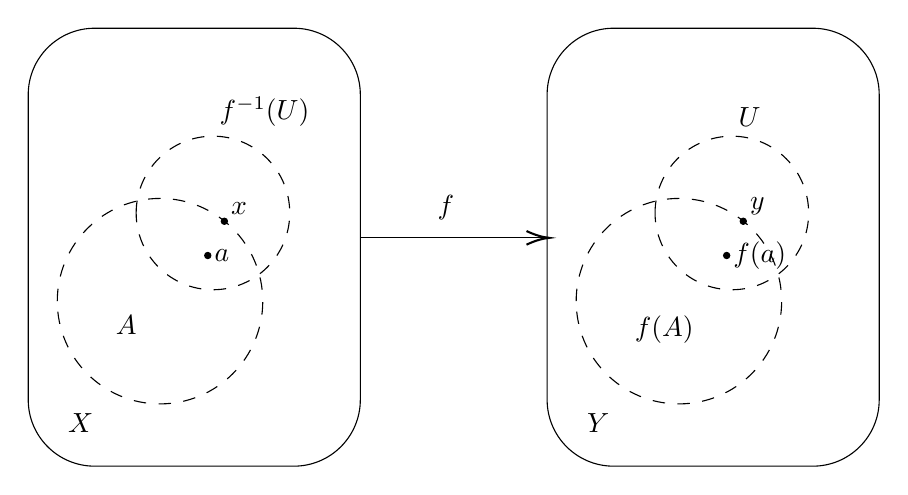
\begin{tikzpicture}[x=0.75pt,y=0.75pt,yscale=-1,xscale=1]
\draw   (41,71) .. controls (41,53.33) and (55.33,39) .. (73,39) -- (169,39) .. controls (186.67,39) and (201,53.33) .. (201,71) -- (201,218) .. controls (201,235.67) and (186.67,250) .. (169,250) -- (73,250) .. controls (55.33,250) and (41,235.67) .. (41,218) -- cycle ;
\draw    (201,140) -- (290,140) ;
\draw [shift={(292,140)}, rotate = 180] [color={rgb, 255:red, 0; green, 0; blue, 0 }  ][line width=0.75]    (10.93,-3.29) .. controls (6.95,-1.4) and (3.31,-0.3) .. (0,0) .. controls (3.31,0.3) and (6.95,1.4) .. (10.93,3.29)   ;
\draw  [dash pattern={on 4.5pt off 4.5pt}] (55,170.5) .. controls (55,143.16) and (77.16,121) .. (104.5,121) .. controls (131.84,121) and (154,143.16) .. (154,170.5) .. controls (154,197.84) and (131.84,220) .. (104.5,220) .. controls (77.16,220) and (55,197.84) .. (55,170.5) -- cycle ;
\draw  [dash pattern={on 4.5pt off 4.5pt}] (93,128) .. controls (93,107.57) and (109.57,91) .. (130,91) .. controls (150.43,91) and (167,107.57) .. (167,128) .. controls (167,148.43) and (150.43,165) .. (130,165) .. controls (109.57,165) and (93,148.43) .. (93,128) -- cycle ;
\draw  [fill={rgb, 255:red, 0; green, 0; blue, 0 }  ,fill opacity=1 ] (134,132) .. controls (134,131.17) and (134.67,130.5) .. (135.5,130.5) .. controls (136.33,130.5) and (137,131.17) .. (137,132) .. controls (137,132.83) and (136.33,133.5) .. (135.5,133.5) .. controls (134.67,133.5) and (134,132.83) .. (134,132) -- cycle ;
\draw  [fill={rgb, 255:red, 0; green, 0; blue, 0 }  ,fill opacity=1 ] (126,148.5) .. controls (126,147.67) and (126.67,147) .. (127.5,147) .. controls (128.33,147) and (129,147.67) .. (129,148.5) .. controls (129,149.33) and (128.33,150) .. (127.5,150) .. controls (126.67,150) and (126,149.33) .. (126,148.5) -- cycle ;
\draw   (291,71) .. controls (291,53.33) and (305.33,39) .. (323,39) -- (419,39) .. controls (436.67,39) and (451,53.33) .. (451,71) -- (451,218) .. controls (451,235.67) and (436.67,250) .. (419,250) -- (323,250) .. controls (305.33,250) and (291,235.67) .. (291,218) -- cycle ;
\draw  [dash pattern={on 4.5pt off 4.5pt}] (305,170.5) .. controls (305,143.16) and (327.16,121) .. (354.5,121) .. controls (381.84,121) and (404,143.16) .. (404,170.5) .. controls (404,197.84) and (381.84,220) .. (354.5,220) .. controls (327.16,220) and (305,197.84) .. (305,170.5) -- cycle ;
\draw  [dash pattern={on 4.5pt off 4.5pt}] (343,128) .. controls (343,107.57) and (359.57,91) .. (380,91) .. controls (400.43,91) and (417,107.57) .. (417,128) .. controls (417,148.43) and (400.43,165) .. (380,165) .. controls (359.57,165) and (343,148.43) .. (343,128) -- cycle ;
\draw  [fill={rgb, 255:red, 0; green, 0; blue, 0 }  ,fill opacity=1 ] (384,132) .. controls (384,131.17) and (384.67,130.5) .. (385.5,130.5) .. controls (386.33,130.5) and (387,131.17) .. (387,132) .. controls (387,132.83) and (386.33,133.5) .. (385.5,133.5) .. controls (384.67,133.5) and (384,132.83) .. (384,132) -- cycle ;
\draw  [fill={rgb, 255:red, 0; green, 0; blue, 0 }  ,fill opacity=1 ] (376,148.5) .. controls (376,147.67) and (376.67,147) .. (377.5,147) .. controls (378.33,147) and (379,147.67) .. (379,148.5) .. controls (379,149.33) and (378.33,150) .. (377.5,150) .. controls (376.67,150) and (376,149.33) .. (376,148.5) -- cycle ;
\draw (237,118.4) node [anchor=north west][inner sep=0.75pt]    {$f$};
\draw (137.5,130.1) node [anchor=south west] [inner sep=0.75pt]    {$x$};
\draw (129.5,148.5) node [anchor=west] [inner sep=0.75pt]    {$a$};
\draw (132,87.6) node [anchor=south west] [inner sep=0.75pt]    {$f^{-1}( U)$};
\draw (82,176.4) node [anchor=north west][inner sep=0.75pt]    {$A$};
\draw (59,223.4) node [anchor=north west][inner sep=0.75pt]    {$X$};
\draw (387.5,130.1) node [anchor=south west] [inner sep=0.75pt]    {$y$};
\draw (379.5,148.5) node [anchor=west] [inner sep=0.75pt]    {$f( a)$};
\draw (382,87.6) node [anchor=south west] [inner sep=0.75pt]    {$U$};
\draw (332,176.4) node [anchor=north west][inner sep=0.75pt]    {$f( A)$};
\draw (309,223.4) node [anchor=north west][inner sep=0.75pt]    {$Y$};
\end{tikzpicture}
\caption{命题2.3之证明图示}
			\end{figure}
			如上图,\tl{$\forall U\subset_{open}\tpj(y\in U)$},由\lei{2}可知$f^{-1}(U)$是开集,又由于$x\in f^{-1}(U)\st f(x)=y\in U$,因此$x\in f^{-1}(U)$。另外由于$\exists x\in f^{-1}(U)$,则有:
			$$(f^{-1}(U)\chadiao \dkh{x})\cap A\neq \emptyset$$这说明除了$x$外,$\exists a\in (f^{-1}(U))\cap A$,即$f(a)\in U, f(a)\in f(A)$,因此$U\cap f(A)\neq \emptyset$,又由于$y\notin f(A)$,即\tl{$(U\chadiao\dkh{y})\cap f(A) \neq \emptyset$},因此$y$是$f(A)$的极限点。
			\end{enumerate}
		\end{enumerate}
		\item[[\lei{$4\Rightarrow 5$}]]:直接在\lei{4}中取$A = f^{-1}(B)$,那么立马有:
		\begin{equation*}
			f(\overline{f^{-1}(B)}) \subset \overline{f(f^{-1}(B))}=B\subset \overline{B}
		\end{equation*}
		因此两边作用$f^{-1}$则得证。
		\item[[\lei{$5\Rightarrow 6$}]]:$\forall F\subset_{closed} Y$,根据\lei{5},然后由于$F$是闭集,所以$\overline{f^{-1}(F)}\subset f^{-1}(\overline{F}) = f^{-1}(F)$,而这一等式的反向是自然成立的,所以有$\overline{f^{-1}(F)}= f^{-1}(F)$。因此$f^{-1}(F)$是闭集。
		\item[[\lei{$6\Rightarrow 2$}]]:任取$U\subset_{open}Y$,注意到$f^{-1}(U) \sqcup f^{-1}(Y\chadiao U) = X$,这里的无交并是因为$f$是映射。因此立马可以得到$$f^{-1}(U) = X\chadiao f^{-1}(Y\chadiao U) $$由于$f^{-1}(Y\chadiao U)$是闭集,因此$f^{-1}(U) = X\chadiao f^{-1}(Y\chadiao U)$是开集。
	\end{enumerate}
\end{proof}
\subsection{拓扑空间中的极限与Hausdorff\footnote{费利克斯·豪斯多夫(德语:Felix Hausdorff,1868年11月8日-1942年1月26日),德国数学家。他是拓扑学的创始人之一,并且对集合论和泛函分析都贡献不少。他定义和研究偏序集、豪斯多夫空间和豪斯多夫维,证明豪斯多夫极大定理。他以笔名Paul Mongré出版哲学和文学作品。}空间}
研究连续性,是和极限密不可分的,下面开始定义极限。
\begin{definition}[极限]\label{c2-d2}
	设$X$是一个拓扑空间,$\dkh{x_{n}}\subset X$是$X$内的一个序列,如果对于$\forall U\subset_{open} X(x\in U) , \exists N,\st \forall n>N,x_{n}\in U$,
	则把$x\in X$称为$\dkh{x_{n}}$的一个\gn{极限}。
\end{definition}
\begin{note}
以上之所以说定义出来的极限是“一个”极限。是因为由此定义出的极限不唯一,其根本在于拓扑空间$X$中的点不一定可以分离,也就是所谓的\textbf{分离性}不一定存在。下面给出一个例子来说明这点。	
\end{note}
\begin{example}[定义\ref{c2-d2}中定义出的极限并不唯一]
\label{c2-e4}
	设$X = \dkh{0,1},\tp = \dkh{\dkh{0},\dkh{0,1},\emptyset}$,设$x_{n} = 0 , n =1,2,\cdots$, 因此:$\displaystyle\lim_{n}x_{n} = 0$是显然的,并且由于$U = \dkh{0,1}$是唯一包含$1$的开集,所以$\displaystyle\lim_{n}x_{n} = 1$。因此这个极限有两个值。
\end{example}

这样就非常的不好啊,仔细想来,在$\mathbb{R}$中我们可以有唯一的极限,这是因为$\mathbb{R}$很牛,里面有很多结构,比如有欧氏度量,而且还是全序域,还有线性结构。一般的拓扑空间不能做到极限唯一,肯定是因为其少了什么东西,这种东西就是所谓的\textbf{分离性}。增加的方法有很多,比如下面的\lei{T2}分离公理。

\begin{definition}[Hausdorff空间]
	设$X$为一个拓扑空间,如果$\forall x_{1},x_{2}\in X,x_{1} \neq x_{2} , \exists$开集$U_{1} , U_{2},\st x_{1}\in U_{1},x_{2}\in U_{2}$且$U_{1}\cap U_{2}=\emptyset$,则称$X$为一个\gn{Hausdorff空间}\footnote{这也称为拓扑空间$X$满足\gn{T2分离公理}。}。
\end{definition}
\begin{proposition}
	设$X$为一个Hausdorff空间,$\dkh{x_{n}}\subset X$则若$x_{n}$的极限存在,则$\dkh{x_{n}}$的极限唯一,并记之为$\displaystyle\lim_{n}x_{n}$。
\end{proposition}
\begin{proof}
	反设$\lim_{n}x_{n} = y_{1}$和$\lim_{n}x_{n} = y_{2}\neq y_{1}$同时成立,那么根据定义就$\exists N = \max\dkh{N_{1},N_{2}}  \st  $对$\forall n>N, x_{n}\in U_{1}$和$x_{n}\in U_{1}$同时成立,又由于$X$为一个Hausdorff空间,则$x_{n}\in U_{1}\cap U_{2}=\emptyset$,矛盾。
\end{proof}
\begin{example}[例\ref{c2-e4}中极限不存在的原因]
	设$X = \dkh{0,1},\tp = \dkh{\dkh{0},\dkh{0,1},\emptyset}$,则$\tp$不是Hausdorff空间。
	
	这是因为取$y_{1} = 0,y_{2} = 1$,那么$y_{2} \in \dabing_{open}$只只存在一种情况:$y_{2}\in \dkh{0,1}$,此时$U\cap \dkh{y_{1}}=\emptyset$。
\end{example}
\begin{example}[度量空间都是Hausdorff空间]
	设$(X,\rho)$为一个度量空间,$x_{1},x_{2}\in X,x_{1}\neq x_{2}$,设$\rho = \rho(x_{1},x_{2})>0$,令$U_{1} = B(x_{1},\dfrac{\rho}{2}),U_{2} = B(x_{2},\dfrac{\rho}{2})$,那么$U_{1}\cap U_{2}=\emptyset$。
	\begin{figure}[h]
	\centering
\tikzset{every picture/.style={line width=0.75pt}}
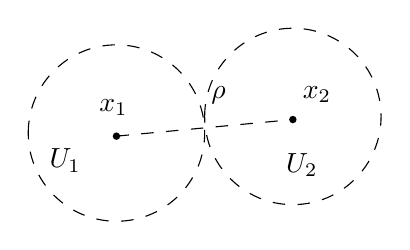
\begin{tikzpicture}[x=0.75pt,y=0.75pt,yscale=-1,xscale=1]
\draw  [dash pattern={on 4.5pt off 4.5pt}] (100,154) .. controls (100,130.53) and (119.03,111.5) .. (142.5,111.5) .. controls (165.97,111.5) and (185,130.53) .. (185,154) .. controls (185,177.47) and (165.97,196.5) .. (142.5,196.5) .. controls (119.03,196.5) and (100,177.47) .. (100,154) -- cycle ;
\draw  [fill={rgb, 255:red, 0; green, 0; blue, 0 }  ,fill opacity=1 ] (141,155.5) .. controls (141,154.67) and (141.67,154) .. (142.5,154) .. controls (143.33,154) and (144,154.67) .. (144,155.5) .. controls (144,156.33) and (143.33,157) .. (142.5,157) .. controls (141.67,157) and (141,156.33) .. (141,155.5) -- cycle ;
\draw  [dash pattern={on 4.5pt off 4.5pt}] (185,146) .. controls (185,122.53) and (204.03,103.5) .. (227.5,103.5) .. controls (250.97,103.5) and (270,122.53) .. (270,146) .. controls (270,169.47) and (250.97,188.5) .. (227.5,188.5) .. controls (204.03,188.5) and (185,169.47) .. (185,146) -- cycle ;
\draw  [fill={rgb, 255:red, 0; green, 0; blue, 0 }  ,fill opacity=1 ] (226,147.5) .. controls (226,146.67) and (226.67,146) .. (227.5,146) .. controls (228.33,146) and (229,146.67) .. (229,147.5) .. controls (229,148.33) and (228.33,149) .. (227.5,149) .. controls (226.67,149) and (226,148.33) .. (226,147.5) -- cycle ;
\draw  [dash pattern={on 4.5pt off 4.5pt}]  (142.5,155.5) -- (227.5,147.5) ;
\draw (109,160.4) node [anchor=north west][inner sep=0.75pt]    {$U_{1}$};
\draw (133,136.4) node [anchor=north west][inner sep=0.75pt]    {$x_{1}$};
\draw (231,130.4) node [anchor=north west][inner sep=0.75pt]    {$x_{2}$};
\draw (223,162.4) node [anchor=north west][inner sep=0.75pt]    {$U_{2}$};
\draw (187,130.4) node [anchor=north west][inner sep=0.75pt]    {$\rho $};
\end{tikzpicture}
\caption{例2.6之图示}
\end{figure}
更加准确一点儿说就是,反设$x\in U_{1}\cap U_{2}$,$\rho(x_{1},x_{2})\leq \rho(x_{1},x)+\rho(x,x_{2})\leq \dfrac{\rho}{2}+\dfrac{\rho}{2}$,矛盾!
\end{example}

在分析学中,如果一个函数连续,那么说明函数符号和极限号是可以交换的,即极限号可以取到函数里面去。即:
$$f(x)\text{连续}~\Rightarrow ~\lim_{\mathcal{B}}f(x) = f(\lim_{\mathcal{B}} x)$$
\begin{proposition}
	设$X,Y$皆为Hausdorff空间,映射$f:X\longrightarrow Y$是连续映射,$\dkh{x_{n}}\subset X,\lim_{n}x_{n} = x_{0} ,  \lim_{n}f(x_{n})=y_{0}$,则$\lim_{n}f(x_{n}) = f(\lim_{n}x_{n}) \in Y$
\end{proposition}
\begin{proof}
	这个证明很显然,根据定义,我们只需要证明$\forall U\subset_{open} Y(f(\lim_{n}x_{n})\in U)$,则$\exists N ,n>N,f(x_{n})\in U$。
	
	任取\tl{$U\subset_{open} Y(f(\lim_{n}x_{n})\in U)$},由于$f$是连续映射,所以必然$\lim_{n}x_{n}\in f^{-1}(U)\subset_{open} X$,所以就有:$\exists N,\st n>N,x_{n}\in f^{-1}(U)$即\tl{$f(x_{n})\in U$}。
\end{proof}
\begin{definition}[同胚]
	设$X,Y$是两个拓扑空间,$f:X\longrightarrow Y$如果:
	\begin{enumerate}
		\item $f$是双射。
		\item $f$连续。
		\item $f^{-1}$连续。
	\end{enumerate}
	那么就称映射$f$为一个\gn{同胚}(\gn{homeomorphism})。
\end{definition}

在这个定义中,\lei{2}和\lei{3}真是十分奇怪,怎么会有连续映射的逆映射不连续的呢?下面给出了一个复变函数中的例子来进行说明。
\begin{example}[存在连续映射之逆映射不连续]
设映射为:
\begin{equation*}
	\begin{aligned}
		f:[0,1)&\longrightarrow \mathbb{C}\\
		t&\longmapsto e^{2\pi i t}
	\end{aligned}
\end{equation*}
该映射之逆映射不连续。

\begin{figure}[h]
	\centering
\tikzset{every picture/.style={line width=0.75pt}}\begin{tikzpicture}[x=0.75pt,y=0.75pt,yscale=-1,xscale=1,scale=0.8]
\draw    (72,160) -- (189,160) -- (203,160) (106,156) -- (106,164)(140,156) -- (140,164)(174,156) -- (174,164) ;
\draw [shift={(205,160)}, rotate = 180] [color={rgb, 255:red, 0; green, 0; blue, 0 }  ][line width=0.75]    (10.93,-3.29) .. controls (6.95,-1.4) and (3.31,-0.3) .. (0,0) .. controls (3.31,0.3) and (6.95,1.4) .. (10.93,3.29)   ;
\draw    (249,160) -- (370,160) ;
\draw [shift={(372,160)}, rotate = 180] [color={rgb, 255:red, 0; green, 0; blue, 0 }  ][line width=0.75]    (10.93,-3.29) .. controls (6.95,-1.4) and (3.31,-0.3) .. (0,0) .. controls (3.31,0.3) and (6.95,1.4) .. (10.93,3.29)   ;
\draw    (407,160) -- (577,160) ;
\draw [shift={(579,160)}, rotate = 180] [color={rgb, 255:red, 0; green, 0; blue, 0 }  ][line width=0.75]    (10.93,-3.29) .. controls (6.95,-1.4) and (3.31,-0.3) .. (0,0) .. controls (3.31,0.3) and (6.95,1.4) .. (10.93,3.29)   ;
\draw    (493,244.5) -- (493,72) ;
\draw [shift={(493,70)}, rotate = 90] [color={rgb, 255:red, 0; green, 0; blue, 0 }  ][line width=0.75]    (10.93,-3.29) .. controls (6.95,-1.4) and (3.31,-0.3) .. (0,0) .. controls (3.31,0.3) and (6.95,1.4) .. (10.93,3.29)   ;
\draw   (436,160) .. controls (436,128.52) and (461.52,103) .. (493,103) .. controls (524.48,103) and (550,128.52) .. (550,160) .. controls (550,191.48) and (524.48,217) .. (493,217) .. controls (461.52,217) and (436,191.48) .. (436,160) -- cycle ;
\draw  [draw opacity=0] (172.2,149.74) .. controls (173.36,152.94) and (174,156.4) .. (174,160) .. controls (174,163.6) and (173.36,167.06) .. (172.2,170.26) -- (144,160) -- cycle ; \draw   (172.2,149.74) .. controls (173.36,152.94) and (174,156.4) .. (174,160) .. controls (174,163.6) and (173.36,167.06) .. (172.2,170.26) ;  
\draw    (409,192) .. controls (375.17,243.74) and (256.2,244) .. (211.67,191.79) ;
\draw [shift={(211,191)}, rotate = 50.3] [color={rgb, 255:red, 0; green, 0; blue, 0 }  ][line width=0.75]    (10.93,-3.29) .. controls (6.95,-1.4) and (3.31,-0.3) .. (0,0) .. controls (3.31,0.3) and (6.95,1.4) .. (10.93,3.29)   ;
\draw (102,162.4) node [anchor=north west][inner sep=0.75pt]    {$0$};
\draw (138.5,162.4) node [anchor=north west][inner sep=0.75pt]    {$t$};
\draw (176,162.4) node [anchor=north west][inner sep=0.75pt]    {$1$};
\draw (528,95.4) node [anchor=north west][inner sep=0.75pt]    {$e^{2\pi it}$};
\draw (538,198.4) node [anchor=north west][inner sep=0.75pt]    {$|z|=1$};
\draw (306,137.4) node [anchor=north west][inner sep=0.75pt]    {$f$};
\draw (300,207.4) node [anchor=north west][inner sep=0.75pt]    {$f^{-1}$};
\draw (581,163.4) node [anchor=north west][inner sep=0.75pt]    {$x$};
\draw (495,73.4) node [anchor=north west][inner sep=0.75pt]    {$y$};
\draw (495,160.65) node [anchor=north west][inner sep=0.75pt]    {$o$};
\end{tikzpicture}
\caption{例2.7中的映射}
\end{figure}

这是为什么呢,很显然,该映射$f$是一个连续映射,但是$f^{-1}$不连续,这是因为从$t=0$按照逆时针走,是$t$自$0$增大的过程,但是若顺时针走动,幅角从$0$突然变到比$2\pi$小一点点,$t$会由$0$瞬间变到$1$的周围,导致不连续的事情发生。
\end{example}
\begin{example}[球极投影]\label{c2-e8}
	考虑$S^{2} = \dkh{(x,y,z)|x^{2}+y^{2}+z^{2} = 1}$,北极点为$P = (0,0,1)$。映射:
	\begin{equation*}
		\begin{aligned}
			h:S^{2}\chadiao P&\longrightarrow \mathbb{R}^{2}\\
			(x,y,z)&\longmapsto (u,v)
		\end{aligned}
	\end{equation*}
	其中$\mathbb{R}^{2}$赋予欧氏拓扑,而$S^{2}\chadiao P$赋予子空间拓扑。
	\begin{figure}[h]
		\centering
\tikzset{every picture/.style={line width=0.75pt}}
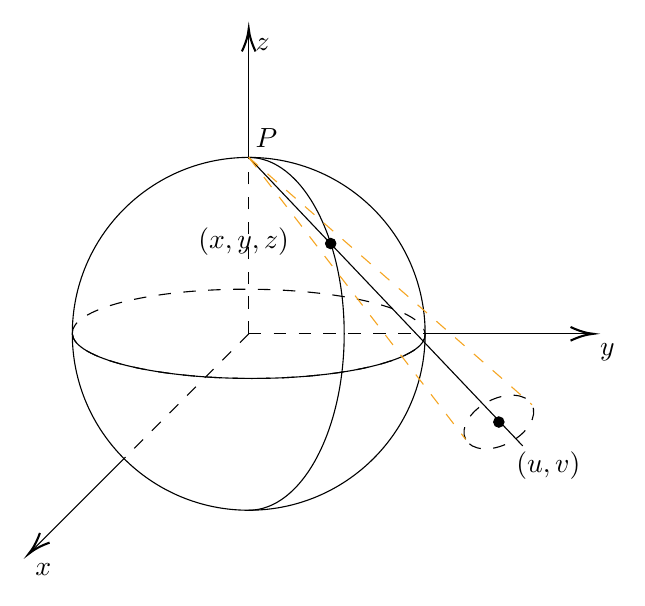
\begin{tikzpicture}[x=0.75pt,y=0.75pt,yscale=-1,xscale=1]
\draw   (121,162) .. controls (121,115.06) and (159.06,77) .. (206,77) .. controls (252.94,77) and (291,115.06) .. (291,162) .. controls (291,208.94) and (252.94,247) .. (206,247) .. controls (159.06,247) and (121,208.94) .. (121,162) -- cycle ;
\draw  [draw opacity=0] (291,162) .. controls (291.83,173.87) and (254.45,183.5) .. (207.5,183.5) .. controls (160.56,183.5) and (121.83,173.87) .. (121,162) -- (206,162) -- cycle ; \draw   (291,162) .. controls (291.83,173.87) and (254.45,183.5) .. (207.5,183.5) .. controls (160.56,183.5) and (121.83,173.87) .. (121,162) ;  
\draw  [draw opacity=0][dash pattern={on 4.5pt off 4.5pt}] (121,162) .. controls (120.17,150.13) and (157.55,140.5) .. (204.5,140.5) .. controls (251.44,140.5) and (290.17,150.13) .. (291,162) .. controls (291.83,173.87) and (254.45,183.5) .. (207.5,183.5) .. controls (160.56,183.5) and (121.83,173.87) .. (121,162) -- (206,162) -- cycle ; \draw  [dash pattern={on 4.5pt off 4.5pt}] (121,162) .. controls (120.17,150.13) and (157.55,140.5) .. (204.5,140.5) .. controls (251.44,140.5) and (290.17,150.13) .. (291,162) .. controls (291.83,173.87) and (254.45,183.5) .. (207.5,183.5) .. controls (160.56,183.5) and (121.83,173.87) .. (121,162) -- cycle ;  
\draw  [draw opacity=0] (206,77) .. controls (231.41,77) and (252,115.06) .. (252,162) .. controls (252,208.94) and (231.41,247) .. (206,247) -- (206,162) -- cycle ; \draw   (206,77) .. controls (231.41,77) and (252,115.06) .. (252,162) .. controls (252,208.94) and (231.41,247) .. (206,247) ;  
\draw  [fill={rgb, 255:red, 0; green, 0; blue, 0 }  ,fill opacity=1 ] (243,118.5) .. controls (243,117.12) and (244.12,116) .. (245.5,116) .. controls (246.88,116) and (248,117.12) .. (248,118.5) .. controls (248,119.88) and (246.88,121) .. (245.5,121) .. controls (244.12,121) and (243,119.88) .. (243,118.5) -- cycle ;
\draw  [dash pattern={on 4.5pt off 4.5pt}]  (206,162) -- (291,162) ;
\draw  [dash pattern={on 4.5pt off 4.5pt}]  (206,162) -- (206,77) ;
\draw  [dash pattern={on 4.5pt off 4.5pt}]  (206,162) -- (146,222) ;
\draw    (146,222) -- (101.41,266.59) ;
\draw [shift={(100,268)}, rotate = 315] [color={rgb, 255:red, 0; green, 0; blue, 0 }  ][line width=0.75]    (10.93,-3.29) .. controls (6.95,-1.4) and (3.31,-0.3) .. (0,0) .. controls (3.31,0.3) and (6.95,1.4) .. (10.93,3.29)   ;
\draw    (291,162) -- (370,162) ;
\draw [shift={(372,162)}, rotate = 180] [color={rgb, 255:red, 0; green, 0; blue, 0 }  ][line width=0.75]    (10.93,-3.29) .. controls (6.95,-1.4) and (3.31,-0.3) .. (0,0) .. controls (3.31,0.3) and (6.95,1.4) .. (10.93,3.29)   ;
\draw    (206,77) -- (206,17) ;
\draw [shift={(206,15)}, rotate = 90] [color={rgb, 255:red, 0; green, 0; blue, 0 }  ][line width=0.75]    (10.93,-3.29) .. controls (6.95,-1.4) and (3.31,-0.3) .. (0,0) .. controls (3.31,0.3) and (6.95,1.4) .. (10.93,3.29)   ;
\draw    (206,77) -- (338,216) ;
\draw  [fill={rgb, 255:red, 0; green, 0; blue, 0 }  ,fill opacity=1 ] (324,204.5) .. controls (324,203.12) and (325.12,202) .. (326.5,202) .. controls (327.88,202) and (329,203.12) .. (329,204.5) .. controls (329,205.88) and (327.88,207) .. (326.5,207) .. controls (325.12,207) and (324,205.88) .. (324,204.5) -- cycle ;
\draw  [dash pattern={on 4.5pt off 4.5pt}] (310.51,212.85) .. controls (307.66,207.4) and (312.52,199.25) .. (321.35,194.64) .. controls (330.18,190.02) and (339.65,190.7) .. (342.49,196.15) .. controls (345.34,201.6) and (340.48,209.75) .. (331.65,214.36) .. controls (322.82,218.98) and (313.35,218.3) .. (310.51,212.85) -- cycle ;
\draw [color={rgb, 255:red, 245; green, 166; blue, 35 }  ,draw opacity=1 ] [dash pattern={on 4.5pt off 4.5pt}]  (206,77) -- (310.51,212.85) ;
\draw [color={rgb, 255:red, 245; green, 166; blue, 35 }  ,draw opacity=1 ] [dash pattern={on 4.5pt off 4.5pt}]  (206,77) -- (342.49,196.15) ;
\draw (102,271.4) node [anchor=north west][inner sep=0.75pt]    {$x$};
\draw (374,165.4) node [anchor=north west][inner sep=0.75pt]    {$y$};
\draw (208,18.4) node [anchor=north west][inner sep=0.75pt]    {$z$};
\draw (180.5,109.4) node [anchor=north west][inner sep=0.75pt]    {$( x,y,z)$};
\draw (333.65,217.76) node [anchor=north west][inner sep=0.75pt]    {$( u,v)$};
\draw (208,73.6) node [anchor=south west] [inner sep=0.75pt]    {$P$};
\end{tikzpicture}
\caption{球极投影}
	\end{figure}
	下面说明映射$h$是一个同胚,需说明三点:
	\begin{enumerate}
		\item 从$h$的构造来看,$h$显然是双射。
		\item 从$h$的构造来看,$h$也是连续映射(把$S^{2}\chadiao P$中的开集映为$\mathbb{R}^{2}$中的开球)
		\item 下说明$h^{-1}$也是连续映射,观察到$(0,0,1),(x,y,z),(u,v,0)$是三点共线,因此$\exists \lambda\neq 0$,并且有关系式:
		\begin{equation*}
			\lambda(x,y,z-1)=\lambda(u,v,-1)
		\end{equation*}
		解出$x=\lambda u,y=\lambda v,z=1-\lambda$,并考虑$(x,y,z)$在球$x^{2}+y^{2}+z^{2}$上,就有:
		\begin{equation*}
			\lambda^{2}u^{2}+\lambda^{2}v^{2}+(1-\lambda)^{2} = 1
		\end{equation*}
		因此同除$\lambda \neq 0$,得到:
		\begin{equation*}
			\lambda=\dfrac{2}{u^{2}+v^{2}+1}
		\end{equation*}
		这样就知道了$h^{-1}$应该满足下关系式:
		\begin{equation*}
			\begin{aligned}
				h^{-1}:\mathbb{R}^{2}&\longrightarrow S^{2}\chadiao \dkh{P}\\
				(u,v)&\longmapsto \xkh{\dfrac{2u}{u^{2}+v^{2}+1},\dfrac{2v}{u^{2}+v^{2}+1},\dfrac{u^{2}+v^{2}-1}{u^{2}+v^{2}+1}}
			\end{aligned}
		\end{equation*}
		现考虑映射$f$:
		\begin{equation*}
			\begin{aligned}
				f:\mathbb{R}^{2}&\longrightarrow \mathbb{R}^{3}\\
				(u,v)&\longmapsto \xkh{\dfrac{2u}{u^{2}+v^{2}+1},\dfrac{2v}{u^{2}+v^{2}+1},\dfrac{u^{2}+v^{2}-1}{u^{2}+v^{2}+1}}
			\end{aligned}
		\end{equation*}
		
		很明显$f$是一个连续映射。根据我们的命题\ref{c2-m3}可知,$h^{-1}$也是连续映射。
	\end{enumerate}
\end{example}
\section{充满整个空间的曲线-Peano\footnote{朱塞佩·皮亚诺 (意大利语:Giuseppe Peano;1858年8月27日-1932年4月20日)是意大利数学家、逻辑学家、语言学家。}曲线}
本节将给出一个在分析学、拓扑学中都很重要且著名的例子---Peano曲线。

\begin{example}[Peano曲线]\index{Peano曲线}
	设$f:[0,1]\longrightarrow X$是一个连续映射,称之为一个\gn{曲线}。其中$X$设定为三角形$\triangle$(边长为$1$),取$\mathbb{R}^{2}$的子空间拓扑。按照如下方式对Peano曲线进行绘制:
	
	\begin{equation*}
		f:[0,1]\longrightarrow X
	\end{equation*}
	$f_{1}$是这副德行(让点~“匀速率游走为红色的线”~):
	\begin{figure}[h]
		\centering
\tikzset{every picture/.style={line width=0.75pt}}
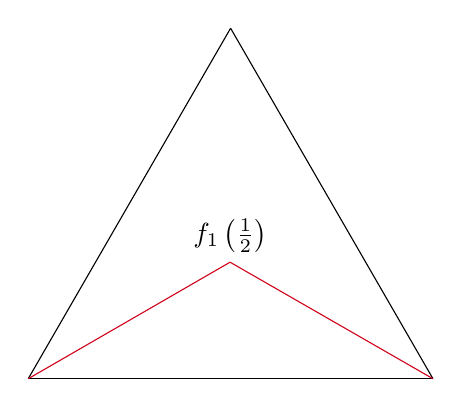
\begin{tikzpicture}[x=0.75pt,y=0.75pt,yscale=-1,xscale=1]
\draw    (151,250) -- (346,250) ;
\draw    (151,250) -- (248.5,81.13) ;
\draw    (248.5,81.13) -- (346,250) ;
\draw [color={rgb, 255:red, 208; green, 2; blue, 27 }  ,draw opacity=1 ]   (151,250) -- (248.25,193.85) ;
\draw [color={rgb, 255:red, 208; green, 2; blue, 27 }  ,draw opacity=1 ]   (248.25,193.85) -- (346,250) ;
\draw (248.25,190.45) node [anchor=south] [inner sep=0.75pt]    {$f_{1}\left(\frac{1}{2}\right)$};
\end{tikzpicture}
\caption{Peano曲线第一步$f_{1}$}
	\end{figure}
	
	接着,把整个三角形按照中点进行连接起来,这样就形成了4个小的并且全等的三角形。然后在每一个三角形里填充$f_1$,但是要注意顺序,$f_2$如下所示:
	
	\begin{figure}[h]
		\centering
\tikzset{every picture/.style={line width=0.75pt}}
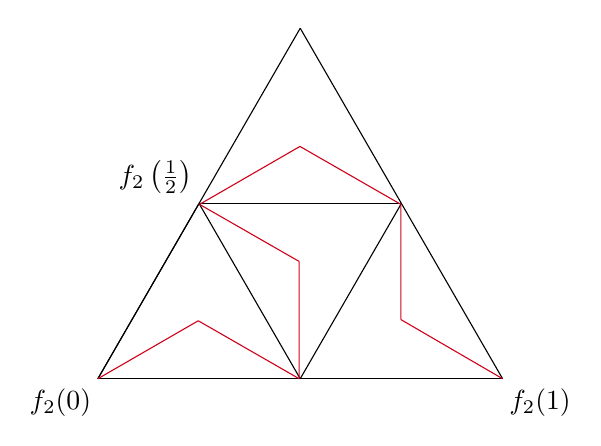
\begin{tikzpicture}[x=0.75pt,y=0.75pt,yscale=-1,xscale=1]
\draw    (171,270) -- (366,270) ;
\draw    (171,270) -- (268.5,101.13) ;
\draw    (268.5,101.13) -- (366,270) ;
\draw    (219.75,185.56) -- (317.25,185.56) ;
\draw    (219.75,185.56) -- (268.5,270) ;
\draw    (317.25,185.56) -- (268.5,270) ;
\draw    (171,270) -- (267.99,270) ;
\draw    (171,270) -- (219.5,186) ;
\draw [color={rgb, 255:red, 208; green, 2; blue, 27 }  ,draw opacity=1 ]   (171,270) -- (219.37,242.07) ;
\draw [color={rgb, 255:red, 208; green, 2; blue, 27 }  ,draw opacity=1 ]   (219.37,242.07) -- (267.99,270) ;
\draw [color={rgb, 255:red, 208; green, 2; blue, 27 }  ,draw opacity=1 ]   (220,186) -- (268.37,158.07) ;
\draw [color={rgb, 255:red, 208; green, 2; blue, 27 }  ,draw opacity=1 ]   (268.37,158.07) -- (316.99,186) ;
\draw [color={rgb, 255:red, 208; green, 2; blue, 27 }  ,draw opacity=1 ]   (267.99,270) -- (268,213.5) ;
\draw [color={rgb, 255:red, 208; green, 2; blue, 27 }  ,draw opacity=1 ]   (220,186) -- (268,213.5) ;
\draw [color={rgb, 255:red, 208; green, 2; blue, 27 }  ,draw opacity=1 ]   (317,241.5) -- (366,270) ;
\draw [color={rgb, 255:red, 208; green, 2; blue, 27 }  ,draw opacity=1 ]   (316.99,186) -- (317,241.5) ;
\draw (169,273.4) node [anchor=north east] [inner sep=0.75pt]    {$f_{2}( 0)$};
\draw (368,273.4) node [anchor=north west][inner sep=0.75pt]    {$f_{2}( 1)$};
\draw (217.75,182.16) node [anchor=south east] [inner sep=0.75pt]    {$f_{2}\left(\frac{1}{2}\right)$};
\end{tikzpicture}
\caption{Peano曲线第二步$f_2$}
	\end{figure}
	
	然后对其中每一个小三角形按照如下替换规则进行替换:
	\begin{figure}[h]
		\centering
\tikzset{every picture/.style={line width=0.75pt}}
\begin{tikzpicture}[x=0.75pt,y=0.75pt,yscale=-1,xscale=1]
\draw    (103,240) -- (298,240) ;
\draw    (103,240) -- (200.5,71.13) ;
\draw    (200.5,71.13) -- (298,240) ;
\draw [color={rgb, 255:red, 208; green, 2; blue, 27 }  ,draw opacity=1 ]   (103,240) -- (200.25,183.85) ;
\draw [color={rgb, 255:red, 208; green, 2; blue, 27 }  ,draw opacity=1 ]   (200.25,183.85) -- (298,240) ;
\draw    (390,241) -- (585,241) ;
\draw    (390,241) -- (487.5,72.13) ;
\draw    (487.5,72.13) -- (585,241) ;
\draw    (438.75,156.56) -- (536.25,156.56) ;
\draw    (438.75,156.56) -- (487.5,241) ;
\draw    (536.25,156.56) -- (487.5,241) ;
\draw    (390,241) -- (486.99,241) ;
\draw    (390,241) -- (438.5,157) ;
\draw [color={rgb, 255:red, 208; green, 2; blue, 27 }  ,draw opacity=1 ]   (390,241) -- (438.37,213.07) ;
\draw [color={rgb, 255:red, 208; green, 2; blue, 27 }  ,draw opacity=1 ]   (438.37,213.07) -- (486.99,241) ;
\draw [color={rgb, 255:red, 208; green, 2; blue, 27 }  ,draw opacity=1 ]   (439,157) -- (487.37,129.07) ;
\draw [color={rgb, 255:red, 208; green, 2; blue, 27 }  ,draw opacity=1 ]   (487.37,129.07) -- (535.99,157) ;
\draw [color={rgb, 255:red, 208; green, 2; blue, 27 }  ,draw opacity=1 ]   (486.99,241) -- (487,184.5) ;
\draw [color={rgb, 255:red, 208; green, 2; blue, 27 }  ,draw opacity=1 ]   (439,157) -- (487,184.5) ;
\draw [color={rgb, 255:red, 208; green, 2; blue, 27 }  ,draw opacity=1 ]   (536,212.5) -- (585,241) ;
\draw [color={rgb, 255:red, 208; green, 2; blue, 27 }  ,draw opacity=1 ]   (535.99,157) -- (536,212.5) ;
\draw    (279,150) -- (404,150) ;
\draw [shift={(406,150)}, rotate = 180] [color={rgb, 255:red, 0; green, 0; blue, 0 }  ][line width=0.75]    (10.93,-3.29) .. controls (6.95,-1.4) and (3.31,-0.3) .. (0,0) .. controls (3.31,0.3) and (6.95,1.4) .. (10.93,3.29)   ;
\draw (342.5,147) node [anchor=south] [inner sep=0.75pt]   [align=left] {替换};
\end{tikzpicture}
\caption{Peano曲线构筑规则}
	\end{figure}
	
	这样我们就得到了$f_3$,以此类推...
	
	\begin{figure}[h]
		\centering


\tikzset{every picture/.style={line width=0.75pt}} %set default line width to 0.75pt        

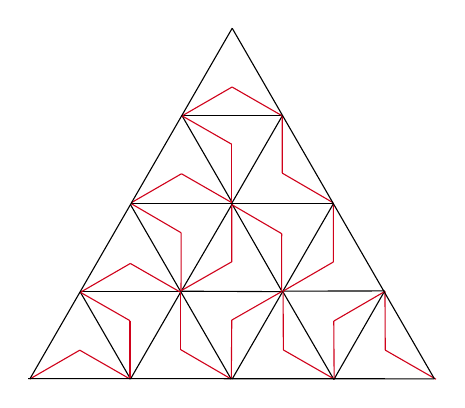
\begin{tikzpicture}[x=0.75pt,y=0.75pt,yscale=-1,xscale=1]
%uncomment if require: \path (0,300); %set diagram left start at 0, and has height of 300

%Straight Lines [id:da4452487886353127] 
\draw    (183.5,134.5) -- (231.99,218.5) ;
%Straight Lines [id:da7452299433041778] 
\draw    (159.25,176.5) -- (207.75,176.5) ;
%Straight Lines [id:da5689545118290742] 
\draw    (159.25,176.5) -- (183.5,218.5) ;
%Straight Lines [id:da4026834110085673] 
\draw    (207.75,176.5) -- (183.5,218.5) ;
%Straight Lines [id:da15211849558958757] 
\draw [color={rgb, 255:red, 208; green, 2; blue, 27 }  ,draw opacity=1 ]   (135,218.5) -- (159.06,204.61) ;
%Straight Lines [id:da013743062828558639] 
\draw [color={rgb, 255:red, 208; green, 2; blue, 27 }  ,draw opacity=1 ]   (159.06,204.61) -- (183.25,218.5) ;
%Straight Lines [id:da6280131962575781] 
\draw [color={rgb, 255:red, 208; green, 2; blue, 27 }  ,draw opacity=1 ]   (159.37,176.72) -- (183.43,162.83) ;
%Straight Lines [id:da4500201719147827] 
\draw [color={rgb, 255:red, 208; green, 2; blue, 27 }  ,draw opacity=1 ]   (183.43,162.83) -- (207.62,176.72) ;
%Straight Lines [id:da9823863695132296] 
\draw [color={rgb, 255:red, 208; green, 2; blue, 27 }  ,draw opacity=1 ]   (183.25,218.5) -- (183.25,190.4) ;
%Straight Lines [id:da9987199864798484] 
\draw [color={rgb, 255:red, 208; green, 2; blue, 27 }  ,draw opacity=1 ]   (159.37,176.72) -- (183.25,190.4) ;
%Straight Lines [id:da5610887461556471] 
\draw [color={rgb, 255:red, 208; green, 2; blue, 27 }  ,draw opacity=1 ]   (207.62,204.32) -- (231.99,218.5) ;
%Straight Lines [id:da44116401718844034] 
\draw [color={rgb, 255:red, 208; green, 2; blue, 27 }  ,draw opacity=1 ]   (207.62,176.72) -- (207.62,204.32) ;
%Straight Lines [id:da20956493721424563] 
\draw    (183.75,134.06) -- (281.25,134.06) ;
%Straight Lines [id:da2458399782846865] 
\draw    (281.25,134.06) -- (232.5,218.5) ;
%Straight Lines [id:da1703054684234142] 
\draw    (232.44,134.25) -- (256.54,176.41) ;
%Straight Lines [id:da7884335868164676] 
\draw    (232.44,134.25) -- (207.98,176.2) ;
%Straight Lines [id:da3252501120078737] 
\draw    (256.54,176.41) -- (207.98,176.2) ;
%Straight Lines [id:da9457474867851912] 
\draw [color={rgb, 255:red, 208; green, 2; blue, 27 }  ,draw opacity=1 ]   (183.88,134.04) -- (207.91,148.05) ;
%Straight Lines [id:da1199139186327054] 
\draw [color={rgb, 255:red, 208; green, 2; blue, 27 }  ,draw opacity=1 ]   (207.91,148.05) -- (207.85,175.98) ;
%Straight Lines [id:da978259216414529] 
\draw [color={rgb, 255:red, 208; green, 2; blue, 27 }  ,draw opacity=1 ]   (232.31,134.47) -- (256.35,148.48) ;
%Straight Lines [id:da37258514563348455] 
\draw [color={rgb, 255:red, 208; green, 2; blue, 27 }  ,draw opacity=1 ]   (256.35,148.48) -- (256.29,176.41) ;
%Straight Lines [id:da5391903142567398] 
\draw [color={rgb, 255:red, 208; green, 2; blue, 27 }  ,draw opacity=1 ]   (207.85,175.98) -- (232.29,162.02) ;
%Straight Lines [id:da49453695674366505] 
\draw [color={rgb, 255:red, 208; green, 2; blue, 27 }  ,draw opacity=1 ]   (232.31,134.47) -- (232.29,162.02) ;
%Straight Lines [id:da6550708204219686] 
\draw [color={rgb, 255:red, 208; green, 2; blue, 27 }  ,draw opacity=1 ]   (232.29,190.12) -- (232.07,218.36) ;
%Straight Lines [id:da7743718768871406] 
\draw [color={rgb, 255:red, 208; green, 2; blue, 27 }  ,draw opacity=1 ]   (256.29,176.41) -- (232.29,190.12) ;
%Straight Lines [id:da9354170106094462] 
\draw    (208.25,91.5) -- (256.75,91.5) ;
%Straight Lines [id:da025313551535410594] 
\draw    (208.25,91.5) -- (232.5,133.5) ;
%Straight Lines [id:da3251539143688129] 
\draw    (256.75,91.5) -- (232.5,133.5) ;
%Straight Lines [id:da3824813283137909] 
\draw [color={rgb, 255:red, 208; green, 2; blue, 27 }  ,draw opacity=1 ]   (184,133.5) -- (208.06,119.61) ;
%Straight Lines [id:da9656996251848466] 
\draw [color={rgb, 255:red, 208; green, 2; blue, 27 }  ,draw opacity=1 ]   (208.06,119.61) -- (232.25,133.5) ;
%Straight Lines [id:da4064095014917104] 
\draw [color={rgb, 255:red, 208; green, 2; blue, 27 }  ,draw opacity=1 ]   (208.37,91.72) -- (232.44,77.82) ;
%Straight Lines [id:da9389690679134728] 
\draw [color={rgb, 255:red, 208; green, 2; blue, 27 }  ,draw opacity=1 ]   (232.44,77.82) -- (256.62,91.72) ;
%Straight Lines [id:da7970229780254066] 
\draw [color={rgb, 255:red, 208; green, 2; blue, 27 }  ,draw opacity=1 ]   (232.25,133.5) -- (232.25,105.39) ;
%Straight Lines [id:da07861937968400046] 
\draw [color={rgb, 255:red, 208; green, 2; blue, 27 }  ,draw opacity=1 ]   (208.37,91.72) -- (232.25,105.39) ;
%Straight Lines [id:da15631925322885132] 
\draw [color={rgb, 255:red, 208; green, 2; blue, 27 }  ,draw opacity=1 ]   (256.63,119.32) -- (281,133.5) ;
%Straight Lines [id:da9532236792775153] 
\draw [color={rgb, 255:red, 208; green, 2; blue, 27 }  ,draw opacity=1 ]   (256.62,91.72) -- (256.63,119.32) ;
%Straight Lines [id:da7940830787810864] 
\draw    (281.48,218.74) -- (256.77,176.18) ;
%Straight Lines [id:da5412492816114032] 
\draw    (281.48,218.74) -- (305.98,176.06) ;
%Straight Lines [id:da14295678090757669] 
\draw    (256.77,176.18) -- (305.98,176.06) ;
%Straight Lines [id:da32223172444353443] 
\draw [color={rgb, 255:red, 208; green, 2; blue, 27 }  ,draw opacity=1 ]   (330.69,218.62) -- (306.24,204.59) ;
%Straight Lines [id:da3858152956993992] 
\draw [color={rgb, 255:red, 208; green, 2; blue, 27 }  ,draw opacity=1 ]   (306.24,204.59) -- (306.11,176.28) ;
%Straight Lines [id:da7564109494509244] 
\draw [color={rgb, 255:red, 208; green, 2; blue, 27 }  ,draw opacity=1 ]   (281.61,218.52) -- (257.15,204.49) ;
%Straight Lines [id:da7222190031387103] 
\draw [color={rgb, 255:red, 208; green, 2; blue, 27 }  ,draw opacity=1 ]   (257.15,204.49) -- (257.02,176.18) ;
%Straight Lines [id:da14163081209457484] 
\draw [color={rgb, 255:red, 208; green, 2; blue, 27 }  ,draw opacity=1 ]   (306.11,176.28) -- (281.44,190.6) ;
%Straight Lines [id:da4232364823033463] 
\draw [color={rgb, 255:red, 208; green, 2; blue, 27 }  ,draw opacity=1 ]   (281.61,218.52) -- (281.44,190.6) ;
%Straight Lines [id:da5379551358921246] 
\draw [color={rgb, 255:red, 208; green, 2; blue, 27 }  ,draw opacity=1 ]   (281.25,162.11) -- (281.27,133.5) ;
%Straight Lines [id:da6496020507310429] 
\draw [color={rgb, 255:red, 208; green, 2; blue, 27 }  ,draw opacity=1 ]   (257.02,176.18) -- (281.25,162.11) ;
%Straight Lines [id:da3996825114817164] 
\draw    (232.5,49.5) -- (135,218.5) ;
%Straight Lines [id:da616059163751844] 
\draw    (134.23,218.29) -- (329.92,218.42) ;
%Straight Lines [id:da4447070580057326] 
\draw    (232.5,49.5) -- (329.92,218.42) ;
\end{tikzpicture}
		\caption{Peano曲线第三步$f_3$}
	\end{figure}
	
	这样一直下去,由于匀速率,$f_n$中小三角形的边长为$\dfrac{1}{2^{n-1}}$,那么我们有以下断言:
	
	\begin{proposition}[Peano曲线]
		\begin{enumerate}
			\item $f_{n} :[0,1]\longrightarrow \triangle$并且有:$f_{n}\rightrightarrows : [0,1]\rightarrow \triangle$,映射$f$是连续映射,将之称为\gn{Peano曲线}。
			\item $f([0,1]) = \triangle$
		\end{enumerate}
	\end{proposition}
	\begin{proof}我们来一条一条证明:
		\begin{enumerate}
			\item $f(t)$是匀速率进行移动,相比较$f_{n+1}$和$f_{n}$,在$f_{n+1}$中的某一点一定要落入比它大四倍的$f_{n}$中。因此我们有$||f_{n+1}(t) - f_{n}(t)||\leq \dfrac{1}{2^{n-1}}$。
			
			
			而$f_n$的边长为$\dfrac{1}{2^{n-1}}$,这就说明在时刻$t$,点一定移动到某个小三角形里,三角形中两点的欧氏距离不超过三角形的边长,即:\tl{$\forall m\geq n+1, ||f_{m}(t) - f_{n}(t)||\leq \dfrac{1}{2^{n-1}} , \forall t\in [0,1]$}。即:
			\begin{equation*}
				\forall \varepsilon >0,\exists N,\st \forall n,m>N,||f_{m}(t) - f_{n}(t)||\leq \varepsilon, \forall t\in [0,1]
			\end{equation*}
			因此在$\mathbb{R}^{2}$中,$\dkh{f_{n}(t)}$是一致收敛的。那么$f$是一个连续映射。
			
			\item $\forall P	\in \triangle ,\forall n\in \mathbb{N}$,通过对$\triangle$的边长进行$2^{n-1}$等分,就得到边长为$\dfrac{1}{2^{n-1}}$的小三角形。则$P$必然落在一个这样的小三角形里,对于$f_n$,必$\exists t_{n},\tl{||f_{n}(t_{n})-P||<\dfrac{1}{2^{n-1}}}$,根据第一点的议论,我们又有$\forall m\geq n+1, \tl{||f_{m}(t) - f_{n}(t)||\leq \dfrac{1}{2^{n-1}}} , \forall t\in [0,1]$,因此:
			\begin{equation*}
				\begin{aligned}
					0\leq ||f(t_{n})-P||&\leq ||f(t_{n})-f_{n}(t_{n})||+||f_{n}(t_{n})-P||\\
					 &\tl{\leq} \dfrac{1}{2^{n-1}}+\dfrac{1}{2^{n-1}} = \dfrac{1}{2^{n}}
				\end{aligned}
			\end{equation*}
			
			当$n\to +\infty$时,$f(t_{n}) \rightarrow P$,因此$P$为$f([0,1])$的极限点。
			
			事实上,\textcolor{myblu}{在欧氏空间$\mathbb{R}^{2}$中,闭区间$[0,1]$是紧集,因此连续映射$f$映射紧集得到的项还是紧集,即欧氏空间$\mathbb{R}^{2}$的闭集。}因此$P\in f([0,1])$,即$f([0,1]) = \triangle$。
		\end{enumerate}
	\end{proof}
\end{example}

%第三章
\chapter{紧性}
紧性是一类非常重要的拓扑性质,在分析中,我们常常利用紧性说明一些真理。紧性和集合开闭、连续都有很大的关联。下面我们首先研究紧性,然后在此基础上推广一些概念,使之更加一般。
\section{开覆盖,紧集,紧子集}
\begin{definition}[开覆盖]
	设$X$为一个拓扑空间,对于拓扑空间$X$中的一族开集$\dkh{U_{i}}_{i\in I}$,如果$$\dabing_{i\in I} U_{i} = X$$那么就把开集族$\dkh{U_{i}}_{i\in I}$称为$X$的一个\gn{开覆盖}。
\end{definition}
\begin{example}[$\mathbb{R}^{3}$中球面$S^{2}$的一组开覆盖]
	以下开集$U_1,U_2$是$\mathbb{R}^{3}$中球面$S^{2}$的一组开覆盖:
	\begin{figure}[h]
		\centering
		

\tikzset{every picture/.style={line width=0.75pt}} %set default line width to 0.75pt        

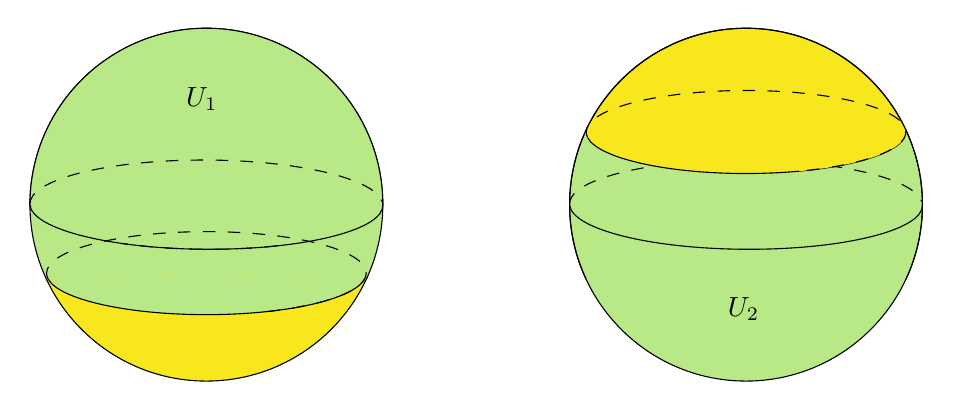
\begin{tikzpicture}[x=0.75pt,y=0.75pt,yscale=-1,xscale=1]
%uncomment if require: \path (0,300); %set diagram left start at 0, and has height of 300

%Shape: Arc [id:dp4877182164030387] 
\draw  [draw opacity=0][fill={rgb, 255:red, 248; green, 231; blue, 28 }  ,fill opacity=1 ] (354.43,119.19) .. controls (367.73,89.6) and (397.46,69) .. (432,69) .. controls (466.25,69) and (495.76,89.25) .. (509.22,118.43) -- (432,154) -- cycle ; \draw   (354.43,119.19) .. controls (367.73,89.6) and (397.46,69) .. (432,69) .. controls (466.25,69) and (495.76,89.25) .. (509.22,118.43) ;  
%Shape: Arc [id:dp23161002882548187] 
\draw  [draw opacity=0][fill={rgb, 255:red, 248; green, 231; blue, 28 }  ,fill opacity=1 ] (249.73,188.45) .. controls (236.51,218.23) and (206.68,239) .. (172,239) .. controls (137.78,239) and (108.28,218.78) .. (94.81,189.64) -- (172,154) -- cycle ; \draw   (249.73,188.45) .. controls (236.51,218.23) and (206.68,239) .. (172,239) .. controls (137.78,239) and (108.28,218.78) .. (94.81,189.64) ;  
%Shape: Arc [id:dp910960502839778] 
\draw  [draw opacity=0][fill={rgb, 255:red, 184; green, 233; blue, 134 }  ,fill opacity=1 ] (248.32,189.67) .. controls (243.31,199.45) and (211.05,207) .. (172,207) .. controls (132.95,207) and (100.69,199.45) .. (95.68,189.67) -- (172,187) -- cycle ; \draw   (248.32,189.67) .. controls (243.31,199.45) and (211.05,207) .. (172,207) .. controls (132.95,207) and (100.69,199.45) .. (95.68,189.67) ;  
%Shape: Arc [id:dp9693162106830377] 
\draw  [draw opacity=0][fill={rgb, 255:red, 184; green, 233; blue, 134 }  ,fill opacity=1 ][dash pattern={on 4.5pt off 4.5pt}] (95.68,189.67) .. controls (95.23,188.79) and (95,187.9) .. (95,187) .. controls (95,175.95) and (129.47,167) .. (172,167) .. controls (214.53,167) and (249,175.95) .. (249,187) .. controls (249,187.9) and (248.77,188.79) .. (248.32,189.67) -- (172,187) -- cycle ; \draw  [dash pattern={on 4.5pt off 4.5pt}] (95.68,189.67) .. controls (95.23,188.79) and (95,187.9) .. (95,187) .. controls (95,175.95) and (129.47,167) .. (172,167) .. controls (214.53,167) and (249,175.95) .. (249,187) .. controls (249,187.9) and (248.77,188.79) .. (248.32,189.67) ;  
%Shape: Arc [id:dp2184763136314598] 
\draw  [draw opacity=0][fill={rgb, 255:red, 184; green, 233; blue, 134 }  ,fill opacity=1 ][dash pattern={on 4.5pt off 4.5pt}] (87,154) .. controls (86.17,142.13) and (123.55,132.5) .. (170.5,132.5) .. controls (217.44,132.5) and (256.17,142.13) .. (257,154) .. controls (257.83,165.87) and (220.45,175.5) .. (173.5,175.5) .. controls (126.56,175.5) and (87.83,165.87) .. (87,154) -- (172,154) -- cycle ; \draw  [dash pattern={on 4.5pt off 4.5pt}] (87,154) .. controls (86.17,142.13) and (123.55,132.5) .. (170.5,132.5) .. controls (217.44,132.5) and (256.17,142.13) .. (257,154) .. controls (257.83,165.87) and (220.45,175.5) .. (173.5,175.5) .. controls (126.56,175.5) and (87.83,165.87) .. (87,154) -- cycle ;  
%Shape: Arc [id:dp049424143239571894] 
\draw  [draw opacity=0][fill={rgb, 255:red, 184; green, 233; blue, 134 }  ,fill opacity=1 ] (87,154) .. controls (87,107.06) and (125.06,69) .. (172,69) .. controls (218.94,69) and (257,107.06) .. (257,154) -- (172,154) -- cycle ; \draw   (87,154) .. controls (87,107.06) and (125.06,69) .. (172,69) .. controls (218.94,69) and (257,107.06) .. (257,154) ;  
%Shape: Arc [id:dp8748762706324542] 
\draw  [draw opacity=0][fill={rgb, 255:red, 184; green, 233; blue, 134 }  ,fill opacity=1 ] (94.93,189.89) .. controls (89.84,178.99) and (87,166.83) .. (87,154) .. controls (87,107.06) and (125.06,69) .. (172,69) .. controls (218.94,69) and (257,107.06) .. (257,154) .. controls (257,166.87) and (254.14,179.08) .. (249.02,190.01) -- (172,154) -- cycle ; \draw   (94.93,189.89) .. controls (89.84,178.99) and (87,166.83) .. (87,154) .. controls (87,107.06) and (125.06,69) .. (172,69) .. controls (218.94,69) and (257,107.06) .. (257,154) .. controls (257,166.87) and (254.14,179.08) .. (249.02,190.01) ;  
%Shape: Arc [id:dp7238984247117861] 
\draw  [draw opacity=0] (257,154) .. controls (257.83,165.87) and (220.45,175.5) .. (173.5,175.5) .. controls (126.56,175.5) and (87.83,165.87) .. (87,154) -- (172,154) -- cycle ; \draw   (257,154) .. controls (257.83,165.87) and (220.45,175.5) .. (173.5,175.5) .. controls (126.56,175.5) and (87.83,165.87) .. (87,154) ;  
%Shape: Arc [id:dp5891897917139242] 
\draw  [draw opacity=0][fill={rgb, 255:red, 184; green, 233; blue, 134 }  ,fill opacity=1 ] (509.07,118.11) .. controls (514.16,129.01) and (517,141.17) .. (517,154) .. controls (517,200.94) and (478.94,239) .. (432,239) .. controls (385.06,239) and (347,200.94) .. (347,154) .. controls (347,141.96) and (349.5,130.51) .. (354.01,120.14) -- (432,154) -- cycle ; \draw   (509.07,118.11) .. controls (514.16,129.01) and (517,141.17) .. (517,154) .. controls (517,200.94) and (478.94,239) .. (432,239) .. controls (385.06,239) and (347,200.94) .. (347,154) .. controls (347,141.96) and (349.5,130.51) .. (354.01,120.14) ;  
%Shape: Arc [id:dp2130503166870723] 
\draw  [draw opacity=0][fill={rgb, 255:red, 184; green, 233; blue, 134 }  ,fill opacity=1 ] (517,154) .. controls (517.83,165.87) and (480.45,175.5) .. (433.5,175.5) .. controls (386.56,175.5) and (347.83,165.87) .. (347,154) -- (432,154) -- cycle ; \draw   (517,154) .. controls (517.83,165.87) and (480.45,175.5) .. (433.5,175.5) .. controls (386.56,175.5) and (347.83,165.87) .. (347,154) ;  
%Shape: Arc [id:dp5006753357361131] 
\draw  [draw opacity=0][fill={rgb, 255:red, 184; green, 233; blue, 134 }  ,fill opacity=1 ][dash pattern={on 4.5pt off 4.5pt}] (347,154) .. controls (346.17,142.13) and (383.55,132.5) .. (430.5,132.5) .. controls (475.47,132.5) and (512.91,141.34) .. (516.7,152.52) -- (432,154) -- cycle ; \draw  [dash pattern={on 4.5pt off 4.5pt}] (347,154) .. controls (346.17,142.13) and (383.55,132.5) .. (430.5,132.5) .. controls (475.47,132.5) and (512.91,141.34) .. (516.7,152.52) ;  
%Shape: Arc [id:dp27854573070484867] 
\draw  [draw opacity=0][fill={rgb, 255:red, 248; green, 231; blue, 28 }  ,fill opacity=1 ] (508.32,121.67) .. controls (503.31,131.45) and (471.05,139) .. (432,139) .. controls (392.95,139) and (360.69,131.45) .. (355.68,121.67) -- (432,119) -- cycle ; \draw   (508.32,121.67) .. controls (503.31,131.45) and (471.05,139) .. (432,139) .. controls (392.95,139) and (360.69,131.45) .. (355.68,121.67) ;  
%Shape: Arc [id:dp5018514725883458] 
\draw  [draw opacity=0][fill={rgb, 255:red, 248; green, 231; blue, 28 }  ,fill opacity=1 ][dash pattern={on 4.5pt off 4.5pt}] (355.68,121.67) .. controls (355.23,120.79) and (355,119.9) .. (355,119) .. controls (355,107.95) and (389.47,99) .. (432,99) .. controls (474.53,99) and (509,107.95) .. (509,119) .. controls (509,127.68) and (487.7,135.07) .. (457.93,137.84) -- (432,119) -- cycle ; \draw  [dash pattern={on 4.5pt off 4.5pt}] (355.68,121.67) .. controls (355.23,120.79) and (355,119.9) .. (355,119) .. controls (355,107.95) and (389.47,99) .. (432,99) .. controls (474.53,99) and (509,107.95) .. (509,119) .. controls (509,127.68) and (487.7,135.07) .. (457.93,137.84) ;  
%Shape: Arc [id:dp019845462128910807] 
\draw  [draw opacity=0] (354.93,189.89) .. controls (349.84,178.99) and (347,166.83) .. (347,154) .. controls (347,107.06) and (385.06,69) .. (432,69) .. controls (478.94,69) and (517,107.06) .. (517,154) .. controls (517,166.87) and (514.14,179.08) .. (509.02,190.01) -- (432,154) -- cycle ; \draw   (354.93,189.89) .. controls (349.84,178.99) and (347,166.83) .. (347,154) .. controls (347,107.06) and (385.06,69) .. (432,69) .. controls (478.94,69) and (517,107.06) .. (517,154) .. controls (517,166.87) and (514.14,179.08) .. (509.02,190.01) ;  
%Shape: Arc [id:dp7763317975452522] 
\draw  [draw opacity=0][dash pattern={on 4.5pt off 4.5pt}] (95.68,189.67) .. controls (95.23,188.79) and (95,187.9) .. (95,187) .. controls (95,175.95) and (129.47,167) .. (172,167) .. controls (214.53,167) and (249,175.95) .. (249,187) .. controls (249,195.68) and (227.7,203.07) .. (197.93,205.84) -- (172,187) -- cycle ; \draw  [dash pattern={on 4.5pt off 4.5pt}] (95.68,189.67) .. controls (95.23,188.79) and (95,187.9) .. (95,187) .. controls (95,175.95) and (129.47,167) .. (172,167) .. controls (214.53,167) and (249,175.95) .. (249,187) .. controls (249,195.68) and (227.7,203.07) .. (197.93,205.84) ;  
%Shape: Arc [id:dp4812470301976983] 
\draw  [draw opacity=0][fill={rgb, 255:red, 184; green, 233; blue, 134 }  ,fill opacity=1 ][dash pattern={on 4.5pt off 4.5pt}] (87,154) .. controls (86.17,142.13) and (123.55,132.5) .. (170.5,132.5) .. controls (215.47,132.5) and (252.91,141.34) .. (256.7,152.52) -- (172,154) -- cycle ; \draw  [dash pattern={on 4.5pt off 4.5pt}] (87,154) .. controls (86.17,142.13) and (123.55,132.5) .. (170.5,132.5) .. controls (215.47,132.5) and (252.91,141.34) .. (256.7,152.52) ;  

% Text Node
\draw (422,197.4) node [anchor=north west][inner sep=0.75pt]    {$U_{2}$};
% Text Node
\draw (161,96.4) node [anchor=north west][inner sep=0.75pt]    {$U_{1}$};


\end{tikzpicture}
\caption{例3.1中的$U_1$与$U_2$}
	\end{figure}
	
	即:$S^{2} = U_{1}\cup U_{2}$。
\end{example}

\begin{definition}[子覆盖]
	若开覆盖$\dkh{U_{i}}_{i\in I}$中可以取出一部分开集,记之为$\dkh{U_{j}}_{j\in J},J\subset I$,且满足$\dabing_{j\in J}U_{j} = X$,则称$\dkh{U_{j}}_{j\in J}$为原先开覆盖的一个\gn{子覆盖};若特别地,$|J|<+\infty$,则称之为原先覆盖的一个\gn{有限子覆盖}。
\end{definition}
\begin{definition}[紧性]
	设$X$为一个拓扑空间,若$\forall X$的开覆盖,存在有限子覆盖,则称$X$是\gn{紧的}。
\end{definition}
下面几个例子说明了紧性对于分析学有一些方便的好处。
\begin{example}[紧性的好处一:便于操作]
	映射$f:[a,b]\longrightarrow \mathbb{R}$连续,则$f([a,b])$有界。
	\begin{proof}
		$f$连续,则$f$局部有界,则$\forall x\in [a,b] , \exists x$的邻域$U_{x}, \st  f|_{U_{x}\cap[a,b]}$有界。
		
		由于$[a,b]$是紧集,所以对于任意的$[a,b]$的开覆盖$\dabing_{x\in [a,b]}U_{x}\supset [a,b] $,则$\exists x_{1},\cdots,x_{n},\st \dabing_{i=1}^{n}U_{x_{i}}\supset [a,b]$,即$f([a,b])$有界。
	\end{proof}
\end{example}
\begin{example}[紧性的好处二:可以高枕无忧地做积分(而不用判断其收敛性)]
如果对于$f$在$\mathbb{R}$中区间$X$($X = [a,b) ~or~ (a,b) ~or~ (a,+\infty)$)进行积分,可能会在边界处出现瑕点,例如广义积分$\int_{a}^{\to +\infty}{\rm{d}}x$不一定收敛,所以这个符号不能够轻松地写下来。

	如果$f\in C([a,b])$,那么就可以对$f$在$[a,b]$上进行积分运算$\int_{a}^{b}f(x){\rm{d}}x$,而这个积分必然是收敛的。
\end{example}
\begin{note}
积分在拓扑学中有非常大的作用。可以借由积分来定义所谓的{\cukai{拓扑不变量}}。这是拓扑学研究的动机之一。	
\end{note}


回忆之前数学分析中的情况,我们是说闭区间$[a,b]$是$\mathbb{R}$中的紧集,但是我们的定义是针对拓扑空间$X$来说的,因此差一个子集和子空间拓扑的区别,因此我们需要下面的概念来进行统一:


\begin{definition}[紧子集]
	设$X$为一个拓扑空间,$Y\subset X$,如果$Y$在子控件拓扑下是紧的,则称$Y$为$X$的一个\gn{紧子集}。
\end{definition}
\begin{note}
以下三点相互等价:
\begin{enumerate}
	\item $Y$是紧集。
	\item 对$\forall Y$的开覆盖,不妨记为$\dkh{U_{i}\cap Y}_{i\in I}$,其中$U_{i}\subset_{open}X$,总可找到有限子覆盖$U_{i_{1}}\cap Y,U_{i_{2}}\cap Y,\cdots,U_{i_{n}}\cap Y, \st  \dabing_{j=1}^{n}U_{i_{j}}\cap Y = Y$
	\item 对$\forall X$中的覆盖$Y$的开子集族$\dkh{U_{i}}_{i\in I}$,可找到$U_{i_{1}},U_{i_{2}},\cdots,U_{i_{n}},\st \dabing_{j=1}^{n}U_{i_{j}}\supset Y$
\end{enumerate}	
\end{note}
\begin{proof}
	这显然啊。
\end{proof}
\begin{theorem}[实数集$\mathbb{R}$中的闭集是紧子集]
	$[a,b]\subset \mathbb{R}$赋予欧氏拓扑,是$\mathbb{R}$中紧子集。
\end{theorem}

\begin{note}
首先我们知道,$\mathbb{R}$	中的闭区间必然是有界的(主要是相对比$\mathbb{R}^{n}$中的闭集不一定是有界集(在某个方向一直没有界))。和下面的定理\ref{c3-t2}相对应。
\end{note}

\begin{proof}
	任取$\mathbb{R}$中的一族开集$\dkh{U_{i}}_{i\in I}\supset [a,b]$,假设其根本不存在有限子覆盖。那么将这个闭区间$[a,b]$一分为二,记其中的一个为$[a_{1},b_{1}]$,这个闭区间当然也没有有限子覆盖。这样一直下去,我们就得到一列闭区间族$\dkh{[a_{n},b_{n}]}_{n\in \mathbb{N}}$,里面的任何一个闭区间都不能被$\dkh{U_{i}}_{i\in I}$中的有限个开集覆盖。且$|b_{n}-a_{n}| =\dfrac{1}{2^{n}} \to 0 (n\to +\infty)$。
	
	根据闭区间套定理,$\exists c\in [a_{n},b_{n}] \subset [a,b], \forall n$,但是对于仅仅一个点$c$,当然有$c\in U_{i_{0}}$。即:$$\exists N,\st [a_{N},b_{N}]\subset U_{i_{0}}$$这与假设矛盾。
\end{proof}

	在这个例子里,$[a,b]$明显是闭集,也是$\mathbb{R}$中的紧子集。反之,$\mathbb{R}$中的紧子集都长成$[a,b]$这样的德行。不长这样的必然不是紧集,比如$(0,1]$并非紧集\footnote{这是因为$\dajiao_{n=2}^{=\infty}(\dfrac{1}{n},2)\cap(0,1] = (0,1]$}。那么自然就会发问:\textbf{一般拓扑空间$X$中的紧子集是否都是闭集?}


\begin{example}[一般拓扑空间中的紧集不一定是闭集]
	设$X=\dkh{0,1},\tp = \dkh{\dkh{0},\dkh{0,1},\emptyset}$对于集合$Y = \dkh{0}$,是$X$中紧集,但是并不是闭集(因为$X\chadiao Y = \dkh{1}\notin \tp$即不是开集)。
\end{example}
很明显的直觉就是,这个玩意不乖是因为没有T2分离公理,所以我们隆重推出以下结论:
\begin{proposition}[Hausdroff空间中的紧集必然是闭集]
	设$Y\subset X$是拓扑空间,$Y$是紧集,那么如果$X$是Hausdroff空间,则$Y$是闭集。
\end{proposition}
\begin{proof}
	即要证$\forall x_{0}\in  X\chadiao Y$,找到一个$Y\subset_{open}X , \st x_{0}\in U\subset X\chadiao Y$。
	
	\begin{figure}[h]
		\centering


\tikzset{every picture/.style={line width=0.75pt}} %set default line width to 0.75pt        

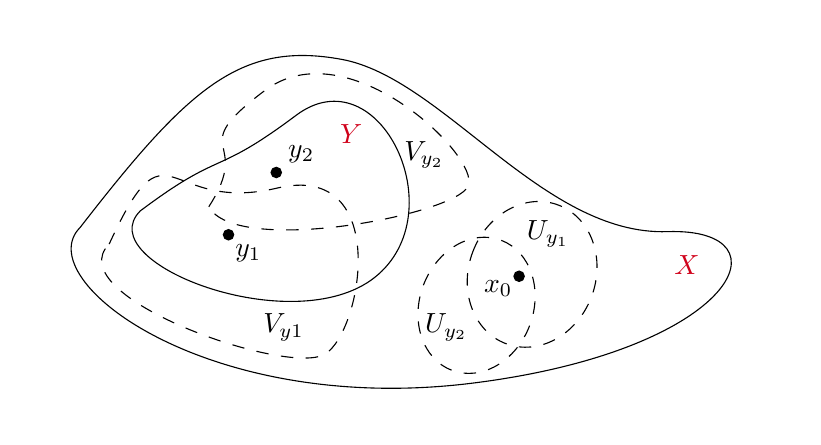
\begin{tikzpicture}[x=0.75pt,y=0.75pt,yscale=-1,xscale=1]
%uncomment if require: \path (0,300); %set diagram left start at 0, and has height of 300

%Curve Lines [id:da012157783454685323] 
\draw    (54,133) .. controls (106,66) and (131,43) .. (180,52) .. controls (229,61) and (277,137) .. (337,135) .. controls (397,133) and (371,192) .. (243,208) .. controls (115,224) and (29,158) .. (54,133) -- cycle ;
%Shape: Circle [id:dp9619535187052062] 
\draw  [fill={rgb, 255:red, 0; green, 0; blue, 0 }  ,fill opacity=1 ] (123,136.5) .. controls (123,135.12) and (124.12,134) .. (125.5,134) .. controls (126.88,134) and (128,135.12) .. (128,136.5) .. controls (128,137.88) and (126.88,139) .. (125.5,139) .. controls (124.12,139) and (123,137.88) .. (123,136.5) -- cycle ;
%Shape: Circle [id:dp5809771479656438] 
\draw  [fill={rgb, 255:red, 0; green, 0; blue, 0 }  ,fill opacity=1 ] (263,156.5) .. controls (263,155.12) and (264.12,154) .. (265.5,154) .. controls (266.88,154) and (268,155.12) .. (268,156.5) .. controls (268,157.88) and (266.88,159) .. (265.5,159) .. controls (264.12,159) and (263,157.88) .. (263,156.5) -- cycle ;
%Shape: Circle [id:dp8252570204737129] 
\draw  [fill={rgb, 255:red, 0; green, 0; blue, 0 }  ,fill opacity=1 ] (146,106.5) .. controls (146,105.12) and (147.12,104) .. (148.5,104) .. controls (149.88,104) and (151,105.12) .. (151,106.5) .. controls (151,107.88) and (149.88,109) .. (148.5,109) .. controls (147.12,109) and (146,107.88) .. (146,106.5) -- cycle ;
%Curve Lines [id:da33996927567313806] 
\draw    (83,125) .. controls (123,95) and (118,109) .. (158,79) .. controls (198,49) and (235,126) .. (196,157) .. controls (157,188) and (58,150) .. (83,125) -- cycle ;
%Curve Lines [id:da6349582936361065] 
\draw  [dash pattern={on 4.5pt off 4.5pt}]  (116,123) .. controls (138,89) and (103,97) .. (143,67) .. controls (183,37) and (247,99) .. (241,113) .. controls (235,127) and (129,147) .. (116,123) -- cycle ;
%Curve Lines [id:da06055669728511659] 
\draw  [dash pattern={on 4.5pt off 4.5pt}]  (68,141) .. controls (97,78) and (94,127) .. (149,114) .. controls (204,101) and (190,183) .. (172,194) .. controls (154,205) and (43,166) .. (68,141) -- cycle ;
%Shape: Ellipse [id:dp5396771508142577] 
\draw  [dash pattern={on 4.5pt off 4.5pt}] (243.17,144.76) .. controls (250.14,126.32) and (268.6,116.21) .. (284.4,122.19) .. controls (300.19,128.16) and (307.35,147.95) .. (300.38,166.39) .. controls (293.4,184.83) and (274.95,194.94) .. (259.15,188.97) .. controls (243.35,183) and (236.2,163.2) .. (243.17,144.76) -- cycle ;
%Shape: Ellipse [id:dp19782369079178785] 
\draw  [dash pattern={on 4.5pt off 4.5pt}] (219.39,160.82) .. controls (225.94,143.51) and (242.71,133.82) .. (256.85,139.16) .. controls (270.99,144.51) and (277.15,162.87) .. (270.61,180.18) .. controls (264.06,197.49) and (247.29,207.18) .. (233.15,201.84) .. controls (219.01,196.49) and (212.85,178.13) .. (219.39,160.82) -- cycle ;

% Text Node
\draw (127.5,139.9) node [anchor=north west][inner sep=0.75pt]    {$y_{1}$};
% Text Node
\draw (153,103.1) node [anchor=south west] [inner sep=0.75pt]    {$y_{2}$};
% Text Node
\draw (141,173.4) node [anchor=north west][inner sep=0.75pt]    {$V_{y1}{}$};
% Text Node
\draw (209,90.4) node [anchor=north west][inner sep=0.75pt]    {$V_{y_{2}}{}$};
% Text Node
\draw (263.5,157.4) node [anchor=north east] [inner sep=0.75pt]    {$x_{0}$};
% Text Node
\draw (268,128.4) node [anchor=north west][inner sep=0.75pt]    {$U_{y_{1}}{}$};
% Text Node
\draw (219,173.4) node [anchor=north west][inner sep=0.75pt]    {$U_{y_{2}}{}$};
% Text Node
\draw (339,145.4) node [anchor=north west][inner sep=0.75pt]  [color={rgb, 255:red, 208; green, 2; blue, 27 }  ,opacity=1 ]  {$X$};
% Text Node
\draw (178,82.4) node [anchor=north west][inner sep=0.75pt]  [color={rgb, 255:red, 208; green, 2; blue, 27 }  ,opacity=1 ]  {$Y$};


\end{tikzpicture}
\caption{命题3.1之示意图}
	\end{figure}
	
	任取$x_{0}\neq y_{1}\in Y$,由于\lanse{$X$是Hausdroff空间},则$\exists V_{y_{1}}(y_{1}\in V_{y_{1}}) , U_{y_{1}}(x_{0}\in U_{y_{1}}),\st V_{y_{1}}\cap U_{y_{1}} = \emptyset$,又由于\lanse{$X$是紧集},任取$Y$的一个开覆盖$\dkh{V_{y_{i}}}_{i}^{\infty}$存在有限子覆盖$\dkh{V_{y_{i}}}_{i}^{n}$,使得\begin{equation}\label{eq3-1}
		\dabing_{i=1}^{n}V_{y_{i}} \supset Y
	\end{equation}
	同时取$U = \dajiao_{j} U_{y_{j}}$,则$$U\cap V_{y_{i}} = \xkh{\dabing_{j}U_{y_{j}}}\cap V_{j_{i}} = \emptyset , \forall i$$
	
	因此$U\subset X\chadiao (\dabing_{i=1}^{n})V_{y_{i}}$,而又有式\ref{eq3-1},因此$U\subset X\chadiao Y$,得证。
	
	
\end{proof}
\begin{proposition}[紧集的闭子集是紧子集]
	设$X$是拓扑空间,$X$是紧集,若则$Y\subset X$是闭子集,则$Y$是紧集。
\end{proposition}
\begin{proof}
	取$X$中$Y$的一族开覆盖$\dkh{U_{i}}_{i\in I}$,即$\dabing_{i\in I}U_{i}\supset Y$,因为$Y$是闭集,所以$U = X\chadiao Y$是开集。又由于$X$是紧集,因此有限覆盖$\dkh{U_{i_{j}}}_{j}^{n}$满足$$(\dabing_{j=1}^{n}U_{i_{j}})\cup U = X$$因此:
	\begin{equation*}
		\begin{aligned}
			Y & = Y\cap X\\
			& = Y\cap\xkh{(\dabing_{j=1}^{n}U_{i_{j}})\cup U}\\
			& = (\dabing_{j=1}^{n}(U_{i_{j}}\cap Y))\cup (Y\cap U)\\
			&=\dabing_{j=1}^{n}(U_{i_{j}}\cap Y)
		\end{aligned}
	\end{equation*}
	因此$Y\subset \dabing_{j=1}^{n}U_{i_{j}}$,得证。
\end{proof}
\begin{theorem}[欧氏空间$\mathbb{R}^{n}$中的紧子集必然是有界闭集]\label{c3-t2}
	设$X\subset \mathbb{R}^{n}$是紧集$\iff X$是有界闭集。
\end{theorem}
\begin{proof}
下分两部分来证明:
	\begin{enumerate}
		\item[[\lei{$\Rightarrow $}]]:设$X\subset \mathbb{R}^{n}$是紧集,则$X\subset \dabing_{i=1}^{+\infty}B_{\mathbb{R}^{n}}(0,i)$,则由于其紧性,$\exists n_{1}<n_{2}<\cdots<n_{k} , \st X\subset \dajiao_{j=1}^{+\infty}B_{\mathbb{R}^{n}}(0,n_{j}) = B_{\mathbb{R}^{n}}(0,n_{k})$,因此$X$有界;又由于$\mathbb{R}^{n}$是Hausdroff空间,因此$X$闭集,得证。
		\item[[\lei{$\Leftarrow $}]]:利用\lanse{闭集套定理}立得,或者利用下一节的\lanse{乘积拓扑}的性质。
	\end{enumerate}
\end{proof}
\section{乘积拓扑}
\subsection{一般般的乘积拓扑}
实际上,在分析学中,我们已经接触到一些与乘积拓扑相关的例子。
\begin{example}[$\mathbb{R}^{2}$中的闭矩形]
	比如集合$[a,b]\times [c,d] = \dkh{(x,y)|a\leq x\leq b,c\leq y\leq d}$,如下图所示:
	\begin{figure}[h]
	\centering
		

\tikzset{every picture/.style={line width=0.75pt}} %set default line width to 0.75pt        

\begin{tikzpicture}[x=0.75pt,y=0.75pt,yscale=-1,xscale=1]
%uncomment if require: \path (0,300); %set diagram left start at 0, and has height of 300

%Shape: Axis 2D [id:dp743347430684322] 
\draw  (50,234) -- (333,234)(78.3,36) -- (78.3,256) (326,229) -- (333,234) -- (326,239) (73.3,43) -- (78.3,36) -- (83.3,43)  ;
%Shape: Rectangle [id:dp6025371871163259] 
\draw   (143,87) -- (248,87) -- (248,160) -- (143,160) -- cycle ;
%Straight Lines [id:da9080465207126023] 
\draw  [dash pattern={on 4.5pt off 4.5pt}]  (248,160) -- (248,234) ;
%Straight Lines [id:da9902909746683768] 
\draw  [dash pattern={on 4.5pt off 4.5pt}]  (143,160) -- (143,234) ;
%Straight Lines [id:da12091642127155033] 
\draw  [dash pattern={on 4.5pt off 4.5pt}]  (143,87) -- (78,87) ;
%Straight Lines [id:da054402093518220784] 
\draw  [dash pattern={on 4.5pt off 4.5pt}]  (143,160) -- (78,160) ;

% Text Node
\draw (337,229.4) node [anchor=north west][inner sep=0.75pt]    {$x$};
% Text Node
\draw (88,22.4) node [anchor=north west][inner sep=0.75pt]    {$ \begin{array}{l}
y\\
\end{array}$};
% Text Node
\draw (80.3,237.4) node [anchor=north west][inner sep=0.75pt]    {$0$};
% Text Node
\draw (76,90.4) node [anchor=north east] [inner sep=0.75pt]    {$d$};
% Text Node
\draw (76,163.4) node [anchor=north east] [inner sep=0.75pt]    {$c$};
% Text Node
\draw (145,237.4) node [anchor=north west][inner sep=0.75pt]    {$a$};
% Text Node
\draw (250,237.4) node [anchor=north west][inner sep=0.75pt]    {$b$};


\end{tikzpicture}
\caption{$\mathbb{R}^{2}$上闭矩形}
	\end{figure}
	
\end{example}
\begin{example}[$\mathbb{R}^{3}$中的圆柱体]
	集合$S^{1}\times [0,1]$,其中$S^{1}=\dkh{(s,y)|x^{2}+y^{2} = 1,(x,y)\in \mathbb{R}^{2}}$。因此上述集合即为:
	\begin{equation*}
		S^{1}\times [0,1] = \dkh{(x,y,z)|x^{2}+y^{2}=1,0\leq z\leq 1}
	\end{equation*}
	即如下图所示:
	\begin{figure}[h]
		\centering
		

\tikzset{every picture/.style={line width=0.75pt}} %set default line width to 0.75pt        

\begin{tikzpicture}[x=0.75pt,y=0.75pt,yscale=-1,xscale=1]
%uncomment if require: \path (0,300); %set diagram left start at 0, and has height of 300

%Shape: Arc [id:dp5867673470206138] 
\draw  [draw opacity=0] (311,154) .. controls (311,154) and (311,154) .. (311,154) .. controls (311.83,165.87) and (274.45,175.5) .. (227.5,175.5) .. controls (180.56,175.5) and (141.83,165.87) .. (141,154) -- (226,154) -- cycle ; \draw   (311,154) .. controls (311,154) and (311,154) .. (311,154) .. controls (311.83,165.87) and (274.45,175.5) .. (227.5,175.5) .. controls (180.56,175.5) and (141.83,165.87) .. (141,154) ;  
%Shape: Arc [id:dp9801525984935566] 
\draw  [draw opacity=0][dash pattern={on 4.5pt off 4.5pt}] (141,154) .. controls (140.17,142.13) and (177.55,132.5) .. (224.5,132.5) .. controls (271.44,132.5) and (310.17,142.13) .. (311,154) -- (226,154) -- cycle ; \draw  [dash pattern={on 4.5pt off 4.5pt}] (141,154) .. controls (140.17,142.13) and (177.55,132.5) .. (224.5,132.5) .. controls (271.44,132.5) and (310.17,142.13) .. (311,154) ;  
%Straight Lines [id:da3611895710460895] 
\draw  [dash pattern={on 4.5pt off 4.5pt}]  (226,154) -- (311,154) ;
%Straight Lines [id:da12024645752757346] 
\draw  [dash pattern={on 4.5pt off 4.5pt}]  (226,154) -- (226,69) ;
%Straight Lines [id:da7833738970612383] 
\draw  [dash pattern={on 4.5pt off 4.5pt}]  (226,154) -- (166,214) ;
%Straight Lines [id:da8528144415780532] 
\draw    (204.5,175.5) -- (133.41,246.59) ;
\draw [shift={(132,248)}, rotate = 315] [color={rgb, 255:red, 0; green, 0; blue, 0 }  ][line width=0.75]    (10.93,-3.29) .. controls (6.95,-1.4) and (3.31,-0.3) .. (0,0) .. controls (3.31,0.3) and (6.95,1.4) .. (10.93,3.29)   ;
%Straight Lines [id:da6274040575457973] 
\draw    (311,154) -- (390,154) ;
\draw [shift={(392,154)}, rotate = 180] [color={rgb, 255:red, 0; green, 0; blue, 0 }  ][line width=0.75]    (10.93,-3.29) .. controls (6.95,-1.4) and (3.31,-0.3) .. (0,0) .. controls (3.31,0.3) and (6.95,1.4) .. (10.93,3.29)   ;
%Straight Lines [id:da17473737450957993] 
\draw    (226,69) -- (226,9) ;
\draw [shift={(226,7)}, rotate = 90] [color={rgb, 255:red, 0; green, 0; blue, 0 }  ][line width=0.75]    (10.93,-3.29) .. controls (6.95,-1.4) and (3.31,-0.3) .. (0,0) .. controls (3.31,0.3) and (6.95,1.4) .. (10.93,3.29)   ;
%Straight Lines [id:da08714079380313722] 
\draw    (311,154) -- (311,70) ;
%Straight Lines [id:da407712841502595] 
\draw    (141,153) -- (141,69) ;
%Shape: Ellipse [id:dp5634621885708664] 
\draw   (141,69) .. controls (141,57.13) and (179.06,47.5) .. (226,47.5) .. controls (272.94,47.5) and (311,57.13) .. (311,69) .. controls (311,80.87) and (272.94,90.5) .. (226,90.5) .. controls (179.06,90.5) and (141,80.87) .. (141,69) -- cycle ;

% Text Node
\draw (134,251.4) node [anchor=north west][inner sep=0.75pt]    {$x$};
% Text Node
\draw (394,157.4) node [anchor=north west][inner sep=0.75pt]    {$y$};
% Text Node
\draw (228,10.4) node [anchor=north west][inner sep=0.75pt]    {$z$};
% Text Node
\draw (228,157.4) node [anchor=north west][inner sep=0.75pt]    {$0$};


\end{tikzpicture}
		\caption{$\mathbb{R}^{3}$上圆柱体}
	\end{figure}
\end{example}
\begin{example}[轮胎面]
	$\mathbb{R}^{3}$中的轮胎面$T$赋予子空间拓扑同胚于乘积拓扑$S^{1}\times S^{1}$,轮胎面$T$如下:
	\begin{figure}[h]
		\centering
		

\tikzset{every picture/.style={line width=0.75pt}} %set default line width to 0.75pt        

\begin{tikzpicture}[x=0.75pt,y=0.75pt,yscale=-1,xscale=1]
%uncomment if require: \path (0,300); %set diagram left start at 0, and has height of 300

%Straight Lines [id:da46665022496354225] 
\draw  [dash pattern={on 4.5pt off 4.5pt}]  (246,166) -- (331,166) ;
%Straight Lines [id:da18171534318477045] 
\draw  [dash pattern={on 4.5pt off 4.5pt}]  (246,166) -- (246,81) ;
%Straight Lines [id:da47464611202042817] 
\draw  [dash pattern={on 4.5pt off 4.5pt}]  (246,166) -- (186,226) ;
%Straight Lines [id:da5273374104748707] 
\draw    (192,220) -- (153.41,258.59) ;
\draw [shift={(152,260)}, rotate = 315] [color={rgb, 255:red, 0; green, 0; blue, 0 }  ][line width=0.75]    (10.93,-3.29) .. controls (6.95,-1.4) and (3.31,-0.3) .. (0,0) .. controls (3.31,0.3) and (6.95,1.4) .. (10.93,3.29)   ;
%Straight Lines [id:da6648718515799088] 
\draw    (331,166) -- (410,166) ;
\draw [shift={(412,166)}, rotate = 180] [color={rgb, 255:red, 0; green, 0; blue, 0 }  ][line width=0.75]    (10.93,-3.29) .. controls (6.95,-1.4) and (3.31,-0.3) .. (0,0) .. controls (3.31,0.3) and (6.95,1.4) .. (10.93,3.29)   ;
%Straight Lines [id:da42233672776782605] 
\draw    (246,112.5) -- (246,21) ;
\draw [shift={(246,19)}, rotate = 90] [color={rgb, 255:red, 0; green, 0; blue, 0 }  ][line width=0.75]    (10.93,-3.29) .. controls (6.95,-1.4) and (3.31,-0.3) .. (0,0) .. controls (3.31,0.3) and (6.95,1.4) .. (10.93,3.29)   ;
%Shape: Ellipse [id:dp840648962114322] 
\draw   (154.17,190.35) .. controls (146.71,162.19) and (181.77,128.46) .. (232.48,115.01) .. controls (283.2,101.57) and (330.36,113.49) .. (337.83,141.65) .. controls (345.29,169.81) and (310.23,203.54) .. (259.52,216.99) .. controls (208.8,230.43) and (161.64,218.51) .. (154.17,190.35) -- cycle ;
%Shape: Ellipse [id:dp5438465257979463] 
\draw   (195.81,179.31) .. controls (191.73,163.92) and (210.89,145.48) .. (238.61,138.13) .. controls (266.33,130.78) and (292.11,137.3) .. (296.19,152.69) .. controls (300.27,168.08) and (281.11,186.52) .. (253.39,193.87) .. controls (225.67,201.22) and (199.89,194.7) .. (195.81,179.31) -- cycle ;
%Shape: Arc [id:dp12641922139401074] 
\draw  [draw opacity=0] (223.67,222.54) .. controls (223.67,222.54) and (223.67,222.54) .. (223.67,222.54) .. controls (219.86,222.03) and (217.53,215.82) .. (218.47,208.65) .. controls (219.41,201.49) and (223.27,196.09) .. (227.09,196.59) -- (225.38,209.56) -- cycle ; \draw   (223.67,222.54) .. controls (223.67,222.54) and (223.67,222.54) .. (223.67,222.54) .. controls (219.86,222.03) and (217.53,215.82) .. (218.47,208.65) .. controls (219.41,201.49) and (223.27,196.09) .. (227.09,196.59) ;  
%Shape: Arc [id:dp22685883519264038] 
\draw  [draw opacity=0][dash pattern={on 4.5pt off 4.5pt}] (227.09,196.59) .. controls (227.09,196.59) and (227.09,196.59) .. (227.09,196.59) .. controls (230.91,197.09) and (233.24,203.31) .. (232.29,210.47) .. controls (231.35,217.64) and (227.49,223.04) .. (223.67,222.54) -- (225.38,209.56) -- cycle ; \draw  [dash pattern={on 4.5pt off 4.5pt}] (227.09,196.59) .. controls (227.09,196.59) and (227.09,196.59) .. (227.09,196.59) .. controls (230.91,197.09) and (233.24,203.31) .. (232.29,210.47) .. controls (231.35,217.64) and (227.49,223.04) .. (223.67,222.54) ;  
%Shape: Arc [id:dp7651170234393176] 
\draw  [draw opacity=0][dash pattern={on 4.5pt off 4.5pt}] (286.92,207.48) .. controls (286.92,207.48) and (286.92,207.48) .. (286.92,207.48) .. controls (284,209.99) and (277.81,207.59) .. (273.1,202.11) .. controls (268.38,196.63) and (266.93,190.16) .. (269.85,187.65) -- (278.38,197.56) -- cycle ; \draw  [dash pattern={on 4.5pt off 4.5pt}] (286.92,207.48) .. controls (286.92,207.48) and (286.92,207.48) .. (286.92,207.48) .. controls (284,209.99) and (277.81,207.59) .. (273.1,202.11) .. controls (268.38,196.63) and (266.93,190.16) .. (269.85,187.65) ;  
%Shape: Arc [id:dp5131264451553017] 
\draw  [draw opacity=0] (269.85,187.65) .. controls (269.85,187.65) and (269.85,187.65) .. (269.85,187.65) .. controls (272.76,185.13) and (278.95,187.54) .. (283.66,193.02) .. controls (288.38,198.49) and (289.83,204.97) .. (286.92,207.48) -- (278.38,197.56) -- cycle ; \draw   (269.85,187.65) .. controls (269.85,187.65) and (269.85,187.65) .. (269.85,187.65) .. controls (272.76,185.13) and (278.95,187.54) .. (283.66,193.02) .. controls (288.38,198.49) and (289.83,204.97) .. (286.92,207.48) ;  
%Shape: Circle [id:dp5855571536160855] 
\draw   (285.5,196) .. controls (285.5,196.28) and (285.72,196.5) .. (286,196.5) .. controls (286.28,196.5) and (286.5,196.28) .. (286.5,196) .. controls (286.5,195.72) and (286.28,195.5) .. (286,195.5) .. controls (285.72,195.5) and (285.5,195.72) .. (285.5,196) -- cycle ;
%Straight Lines [id:da5483092345722265] 
\draw  [dash pattern={on 4.5pt off 4.5pt}]  (246,166) -- (304,223.5) ;
%Straight Lines [id:da23610679539920998] 
\draw  [dash pattern={on 4.5pt off 4.5pt}]  (286,195.5) -- (286,205.48) ;
%Straight Lines [id:da027094385148068723] 
\draw  [dash pattern={on 4.5pt off 4.5pt}]  (286,205.48) -- (326,165.48) ;
%Straight Lines [id:da2575191594724433] 
\draw  [dash pattern={on 4.5pt off 4.5pt}]  (286,205.48) -- (206,205.48) ;
%Shape: Circle [id:dp04176172531136113] 
\draw   (285.5,204.98) .. controls (285.5,205.26) and (285.72,205.48) .. (286,205.48) .. controls (286.28,205.48) and (286.5,205.26) .. (286.5,204.98) .. controls (286.5,204.7) and (286.28,204.48) .. (286,204.48) .. controls (285.72,204.48) and (285.5,204.7) .. (285.5,204.98) -- cycle ;

% Text Node
\draw (154,263.4) node [anchor=north west][inner sep=0.75pt]    {$x$};
% Text Node
\draw (414,169.4) node [anchor=north west][inner sep=0.75pt]    {$y$};
% Text Node
\draw (248,22.4) node [anchor=north west][inner sep=0.75pt]    {$z$};
% Text Node
\draw (244,162.6) node [anchor=south east] [inner sep=0.75pt]    {$0$};
% Text Node
\draw (288.5,192.6) node [anchor=south west] [inner sep=0.75pt]    {$( x,y,z)$};
% Text Node
\draw (246,169.4) node [anchor=north] [inner sep=0.75pt]    {$\theta $};
% Text Node
\draw (204,205.48) node [anchor=east] [inner sep=0.75pt]    {$a$};


\end{tikzpicture}
\caption{轮胎面$T$}
	\end{figure}
	\newpage
	其中$(x,y,z)$可以由两参数$(\theta,\alpha)$来决定,取第一个$S^{1}$为某点$(x,y,z)$向$xoy$平面做投影得到。投影点与$x$轴之夹角为$\theta$:
	\begin{figure}[h]
		\centering
		

\tikzset{every picture/.style={line width=0.75pt}} %set default line width to 0.75pt        

\begin{tikzpicture}[x=0.75pt,y=0.75pt,yscale=-1,xscale=1]
%uncomment if require: \path (0,300); %set diagram left start at 0, and has height of 300

%Shape: Axis 2D [id:dp18065539959509458] 
\draw  (70,149) -- (277,149)(173,41) -- (173,248) (270,144) -- (277,149) -- (270,154) (168,48) -- (173,41) -- (178,48)  ;
%Shape: Circle [id:dp5752488942133569] 
\draw   (119,149) .. controls (119,119.18) and (143.18,95) .. (173,95) .. controls (202.82,95) and (227,119.18) .. (227,149) .. controls (227,178.82) and (202.82,203) .. (173,203) .. controls (143.18,203) and (119,178.82) .. (119,149) -- cycle ;
%Shape: Circle [id:dp149080506500179] 
\draw  [fill={rgb, 255:red, 0; green, 0; blue, 0 }  ,fill opacity=1 ] (215,119) .. controls (215,117.34) and (216.34,116) .. (218,116) .. controls (219.66,116) and (221,117.34) .. (221,119) .. controls (221,120.66) and (219.66,122) .. (218,122) .. controls (216.34,122) and (215,120.66) .. (215,119) -- cycle ;
%Straight Lines [id:da14226355330318952] 
\draw  [dash pattern={on 4.5pt off 4.5pt}]  (173,149) -- (218,119) ;
%Shape: Arc [id:dp8550926156223679] 
\draw  [draw opacity=0] (191.8,136.63) .. controls (194.14,140.18) and (195.5,144.43) .. (195.5,149) -- (173,149) -- cycle ; \draw   (191.8,136.63) .. controls (194.14,140.18) and (195.5,144.43) .. (195.5,149) ;  

% Text Node
\draw (197.5,145.6) node [anchor=south west] [inner sep=0.75pt]    {$\theta $};
% Text Node
\draw (220,115.6) node [anchor=south west] [inner sep=0.75pt]    {$e^{i\theta }$};


\end{tikzpicture}
		\caption{第一个$S^{1}$球面}
	\end{figure}
	
	在小圆中,建立点$(x,y,z)$与$z$轴之间的夹角为$\alpha$:
	
	\begin{figure}[h]
		\centering
		

\tikzset{every picture/.style={line width=0.75pt}} %set default line width to 0.75pt        

\begin{tikzpicture}[x=0.75pt,y=0.75pt,yscale=-1,xscale=1]
%uncomment if require: \path (0,300); %set diagram left start at 0, and has height of 300

%Straight Lines [id:da715868777824265] 
\draw    (100,178) -- (100,51) ;
\draw [shift={(100,49)}, rotate = 90] [color={rgb, 255:red, 0; green, 0; blue, 0 }  ][line width=0.75]    (10.93,-3.29) .. controls (6.95,-1.4) and (3.31,-0.3) .. (0,0) .. controls (3.31,0.3) and (6.95,1.4) .. (10.93,3.29)   ;
%Straight Lines [id:da5936824959340532] 
\draw  [dash pattern={on 4.5pt off 4.5pt}]  (100,178) -- (337,178) ;
%Straight Lines [id:da0558945933767967] 
\draw    (246,178) -- (246,51) ;
\draw [shift={(246,49)}, rotate = 90] [color={rgb, 255:red, 0; green, 0; blue, 0 }  ][line width=0.75]    (10.93,-3.29) .. controls (6.95,-1.4) and (3.31,-0.3) .. (0,0) .. controls (3.31,0.3) and (6.95,1.4) .. (10.93,3.29)   ;
%Shape: Circle [id:dp6756364793613125] 
\draw  [dash pattern={on 4.5pt off 4.5pt}] (192,178) .. controls (192,148.18) and (216.18,124) .. (246,124) .. controls (275.82,124) and (300,148.18) .. (300,178) .. controls (300,207.82) and (275.82,232) .. (246,232) .. controls (216.18,232) and (192,207.82) .. (192,178) -- cycle ;
%Shape: Circle [id:dp722136459883157] 
\draw  [fill={rgb, 255:red, 0; green, 0; blue, 0 }  ,fill opacity=1 ] (281,139) .. controls (281,137.34) and (282.34,136) .. (284,136) .. controls (285.66,136) and (287,137.34) .. (287,139) .. controls (287,140.66) and (285.66,142) .. (284,142) .. controls (282.34,142) and (281,140.66) .. (281,139) -- cycle ;
%Straight Lines [id:da18507445500370823] 
\draw  [dash pattern={on 4.5pt off 4.5pt}]  (246,178) -- (284,139) ;
%Straight Lines [id:da5829910938279133] 
\draw  [dash pattern={on 4.5pt off 4.5pt}]  (284,177.5) -- (284,139) ;
%Straight Lines [id:da17288867127298624] 
\draw  [dash pattern={on 4.5pt off 4.5pt}]  (246,139) -- (284,139) ;
%Shape: Arc [id:dp34543009938456426] 
\draw  [draw opacity=0] (246,165.5) .. controls (249.34,165.5) and (252.38,166.81) .. (254.62,168.95) -- (246,178) -- cycle ; \draw   (246,165.5) .. controls (249.34,165.5) and (252.38,166.81) .. (254.62,168.95) ;  
%Straight Lines [id:da24295335253932926] 
\draw    (246,178) -- (207.48,142.85) ;
\draw [shift={(206,141.5)}, rotate = 42.38] [color={rgb, 255:red, 0; green, 0; blue, 0 }  ][line width=0.75]    (10.93,-3.29) .. controls (6.95,-1.4) and (3.31,-0.3) .. (0,0) .. controls (3.31,0.3) and (6.95,1.4) .. (10.93,3.29)   ;

% Text Node
\draw (171,180.4) node [anchor=north west][inner sep=0.75pt]    {$a$};
% Text Node
\draw (246,181.4) node [anchor=north] [inner sep=0.75pt]    {$A$};
% Text Node
\draw (248,162.1) node [anchor=south west] [inner sep=0.75pt]    {$\alpha $};
% Text Node
\draw (284,180.9) node [anchor=north] [inner sep=0.75pt]    {$r\sin \alpha $};
% Text Node
\draw (213,154.4) node [anchor=north west][inner sep=0.75pt]    {$r$};
% Text Node
\draw (102,52.4) node [anchor=north west][inner sep=0.75pt]    {$z$};
% Text Node
\draw (98,181.4) node [anchor=north east] [inner sep=0.75pt]    {$o$};


\end{tikzpicture}
		\caption{第二个$S^{1}$球面}
	\end{figure}


这样我们可以看出映射$f$:
\begin{equation*}
	\begin{aligned}
		S^{1}\times S^{1} &\longrightarrow T\\
		(e^{i\theta},e^{i\alpha})&\longmapsto ((a+r\sin \alpha)\cos \theta,(a+r\sin \alpha)\sin \theta ,r\cos \alpha)
	\end{aligned}
\end{equation*}
这个映射是一个双射,因此是一个同胚。这说明\lei{$S^{1}\times S^{1} \cong T$}。
\end{example}
下面我们给出乘积拓扑的定义:
\begin{definition}[乘积拓扑]
	设$X,Y$为两个拓扑空间。定义$\tpj$为$X\times Y$上的如下子集族$$\dkh{U\times V|U\subset_{open},V\subset_{open}Y}$$则$\tpj$生成了$X\times Y$上的一个拓扑,该拓扑称为$X\times Y$上的\gn{乘积拓扑}。
\end{definition}
\begin{proof}
	即证明拓扑基$\tpj$生成了$X\times Y$,即证以下两点:
	\begin{enumerate}
		\item $\dabing_{U\times V\in \tpj}U\times V = X\times Y$
		\item $\forall U_{1}\times V_{1},U_{2}\times V_{2}\in \tpj$要证$\forall (x,y)\in (U_{1}\times V_{1})\cap(U_{2}\times V_{2}),\exists U_{3}\times V_{3}\in \st x\in U_{3}\times V_{3}\subset (U_{1}\times V_{1})\cap(U_{2}\times V_{2})$
	\end{enumerate}
	很显然,第一点是显然的,因此我们只需要验证第二点即可。取$U_{3}\times V_{3} = (U_{1}\times V_{1})\cap(U_{2}\times V_{2})$。即:
	\begin{equation*}
		\begin{aligned}
			(U_{1}\times V_{1})\cap(U_{2}\times V_{2})&=\dkh{(x,y)|(x,y)\in U_{1}\times V_{1},(x,y)\in U_{2}\times V_{2}}\\
			&=\dkh{(s,y)|x\in U_{1},x\in U_{2},y\in V_{1},y\in V_{2}}\\
			&=\dkh{(x,y)|(x,y)\in (U_{1}\cap U_{2})\times (V_{1}\cap V_{2})}\\
			&=(U_{1}\cap U_{2})\times (V_{1}\cap V_{2})
		\end{aligned}
	\end{equation*}
	因此得证。
\end{proof}
\begin{note}
按照上面对于乘积拓扑的定义,我们可以继续定义$n$次乘积的乘积拓扑:
\begin{definition}
	设$X_{1},X_{2},\cdots ,X_{n}$为$n$个拓扑空间。那么定义他们的乘积拓扑空间为:
	\begin{equation*}
		X_{1}\times X_{2} \times X_{n} = (((X_{1}\times X_{2})\times X_{3})\times\cdots )\times)\times X_{n}
	\end{equation*}
\end{definition}	
\end{note}
\begin{example}[$n$维欧氏空间中的闭矩体]
	$n$维欧氏空间中的闭矩体:
	\begin{equation*}
		[a_1,b_1]\times[a_2,b_{2}]\times \cdots [a_{n},b_{n}]\subset \mathbb{R}^{n}
	\end{equation*}
\end{example}
\begin{example}[轮胎面]
	实际上刚刚的例子中直接断言说同胚是不讲道理的,因为我们没有给予两个球面直乘之后的空间一个明确的拓扑结构。下面 我们在单位球面$S^{1}$上考虑两个公转角$\theta_{1}$与$\theta_{2}$,那么集合:
	
	\begin{equation*}
		I_{\theta_{1},\theta_{2}} = \dkh{e^{i\theta}|\theta\in [\theta_{1},\theta_2]}
	\end{equation*}
	
	
	\begin{figure}[h]
		\centering
		

\tikzset{every picture/.style={line width=0.75pt}} %set default line width to 0.75pt        

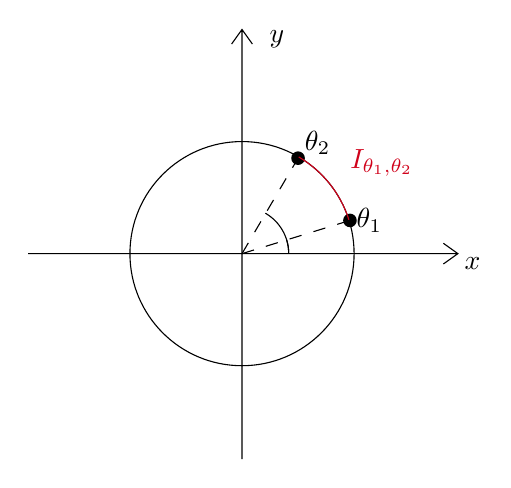
\begin{tikzpicture}[x=0.75pt,y=0.75pt,yscale=-1,xscale=1]
%uncomment if require: \path (0,300); %set diagram left start at 0, and has height of 300

%Shape: Axis 2D [id:dp203175839117822] 
\draw  (90,169) -- (297,169)(193,61) -- (193,268) (290,164) -- (297,169) -- (290,174) (188,68) -- (193,61) -- (198,68)  ;
%Shape: Circle [id:dp12962402600717415] 
\draw   (139,169) .. controls (139,139.18) and (163.18,115) .. (193,115) .. controls (222.82,115) and (247,139.18) .. (247,169) .. controls (247,198.82) and (222.82,223) .. (193,223) .. controls (163.18,223) and (139,198.82) .. (139,169) -- cycle ;
%Shape: Circle [id:dp8795838300142391] 
\draw  [fill={rgb, 255:red, 0; green, 0; blue, 0 }  ,fill opacity=1 ] (242,153) .. controls (242,151.34) and (243.34,150) .. (245,150) .. controls (246.66,150) and (248,151.34) .. (248,153) .. controls (248,154.66) and (246.66,156) .. (245,156) .. controls (243.34,156) and (242,154.66) .. (242,153) -- cycle ;
%Straight Lines [id:da09251544981835158] 
\draw  [dash pattern={on 4.5pt off 4.5pt}]  (193,169) -- (245,153) ;
%Shape: Arc [id:dp5917015531936993] 
\draw  [draw opacity=0] (214.5,162.34) .. controls (215.15,164.45) and (215.5,166.68) .. (215.5,169) .. controls (215.5,169) and (215.5,169) .. (215.5,169) -- (193,169) -- cycle ; \draw   (214.5,162.34) .. controls (215.15,164.45) and (215.5,166.68) .. (215.5,169) .. controls (215.5,169) and (215.5,169) .. (215.5,169) ;  
%Shape: Circle [id:dp9798800064315032] 
\draw  [fill={rgb, 255:red, 0; green, 0; blue, 0 }  ,fill opacity=1 ] (217,123) .. controls (217,121.34) and (218.34,120) .. (220,120) .. controls (221.66,120) and (223,121.34) .. (223,123) .. controls (223,124.66) and (221.66,126) .. (220,126) .. controls (218.34,126) and (217,124.66) .. (217,123) -- cycle ;
%Straight Lines [id:da06492994015485243] 
\draw  [dash pattern={on 4.5pt off 4.5pt}]  (193,169) -- (220,123) ;
%Shape: Arc [id:dp8484317615965473] 
\draw  [draw opacity=0] (204.26,149.52) .. controls (210.98,153.41) and (215.5,160.68) .. (215.5,169) -- (193,169) -- cycle ; \draw   (204.26,149.52) .. controls (210.98,153.41) and (215.5,160.68) .. (215.5,169) ;  
%Shape: Arc [id:dp45409706315033294] 
\draw  [draw opacity=0] (220.33,122.42) .. controls (231.71,129.11) and (240.42,139.85) .. (244.49,152.67) -- (193,169) -- cycle ; \draw  [color={rgb, 255:red, 208; green, 2; blue, 27 }  ,draw opacity=1 ] (220.33,122.42) .. controls (231.71,129.11) and (240.42,139.85) .. (244.49,152.67) ;  

% Text Node
\draw (247,153) node [anchor=west] [inner sep=0.75pt]    {$\theta _{1}$};
% Text Node
\draw (222,122.6) node [anchor=south west] [inner sep=0.75pt]    {$\theta _{2}$};
% Text Node
\draw (299,169.4) node [anchor=north west][inner sep=0.75pt]    {$x$};
% Text Node
\draw (205,60.4) node [anchor=north west][inner sep=0.75pt]    {$y$};
% Text Node
\draw (244,117.4) node [anchor=north west][inner sep=0.75pt]  [color={rgb, 255:red, 208; green, 2; blue, 27 }  ,opacity=1 ]  {$I_{\theta _{1} ,\theta _{2}}{}$};


\end{tikzpicture}
		\caption{$S^{1}$中的拓扑基}
	\end{figure}
	
	那么$I_{\theta_{1},\theta_{2}}$为$S^{1}$的一个拓扑基。且$\dkh{I_{\theta_{1},\theta_{2}}\times I_{\alpha_{1},\alpha_{2}}}$为$S^{1}\times S^{1}$的一个拓扑基。
\end{example}
\subsection{乘积空间上的Universal Property\footnote{中译为\gn{泛性质,有时也称为万有性。范畴论研究泛性质。}}}
以上我们根据乘积空间的性质来定义了乘积拓扑空间,下面让我们挖掘更加一般的性质,定义范畴乘积的概念。
\subsubsection{对于线性空间而言}\label{c3221}
设$V,W$为域$\mathbb{K}$上的两个向量空间。构造$V\times W$为一个$\mathbb{K}$-线性空间:
\begin{enumerate}
	\item $(v_{1},w_{1}) + (v_{2},w_{2}):=(v_{1}+v_{2},w_{1}+w_{2})$
	\item $\lambda \cdot(v,w) = (\lambda v,\lambda w)$
\end{enumerate}
再定义$V\times W$到线性空间$V,W$的两个投影为:
\begin{equation*}
	\begin{aligned}
		\pi_{V} :V\times W&\longrightarrow V\\
		(v,w)&\longmapsto v
	\end{aligned}
\end{equation*}
和\begin{equation*}
	\begin{aligned}
		\pi_{W} :V\times W&\longrightarrow W\\
		(v,w)&\longmapsto w
	\end{aligned}
\end{equation*}
那么$(V\times W,\pi_{V},\pi_{W})$有如下的\lei{Universal Property}:

对于任何一个线性空间$Z$以及线性映射$f:Z\longrightarrow V,g:Z\longrightarrow W,\exists!h:Z\longrightarrow V\times W,\st $下列图表可交换:
\begin{figure}[h]
	\centering
	

\tikzset{every picture/.style={line width=0.75pt}} %set default line width to 0.75pt        

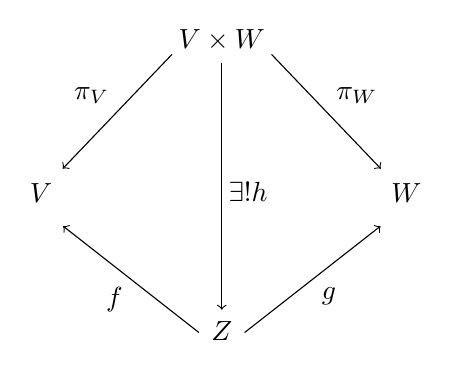
\begin{tikzpicture}[x=0.75pt,y=0.75pt,yscale=-1,xscale=1]
\draw[->]    (289,95) -- (289,214) ;
\draw[->]    (265,91) -- (212.38,146.05) ;
\draw[->]    (313,91) -- (365.62,146.05) ;
\draw[->]    (278,225) -- (212.57,173.73) ;
\draw[->]    (300,225) -- (365.47,173.73) ;
\draw (289,90.6) node [anchor=south] [inner sep=0.75pt]    {$V\times W$};
% Text Node
\draw (289,218.4) node [anchor=north] [inner sep=0.75pt]    {$Z$};
% Text Node
\draw (208.5,157.75) node [anchor=east] [inner sep=0.75pt]    {$V$};
% Text Node
\draw (369.5,157.75) node [anchor=west] [inner sep=0.75pt]    {$W$};
% Text Node
\draw (291,157.25) node [anchor=west] [inner sep=0.75pt]    {$\exists !h$};
% Text Node
\draw (236,115.85) node [anchor=south east] [inner sep=0.75pt]    {$\pi _{V}$};
% Text Node
\draw (343,115.85) node [anchor=south west] [inner sep=0.75pt]    {$\pi _{W}$};
% Text Node
\draw (242.5,202.15) node [anchor=north east] [inner sep=0.75pt]    {$f$};
% Text Node
\draw (336,202.15) node [anchor=north west][inner sep=0.75pt]    {$g$};
\end{tikzpicture}
\end{figure}

\begin{proof}
	定义映射$h$为:
	\begin{equation*}
	\begin{aligned}
		Z&\longrightarrow V\times W\\
		z&\longmapsto (f(z),g(z))
	\end{aligned}
	\end{equation*}
	
	这个映射明显满足以上的图表交换条件,现在问题是这个映射是不是唯一的?答案必然是肯定的,假设另有一个线性映射$\widetilde{h}:Z\longrightarrow V\times W$满足图表交换条件,那么我们有:
	\begin{equation*}
		\pi_{V}\circ \widetilde{h} = f
	\end{equation*}
	\begin{equation*}
		\pi_{W}\circ \widetilde{h} = g
	\end{equation*}
	
	那么对于$\forall z\in Z$,设$\widetilde{h}(z) = (h_{1}(z),h_{2}(z))$,那么由于$\pi_{V}$和$\pi_{W}$是投影,以及上面的性质有:
	\begin{equation*}
		f(z) = \pi_{V}(\widetilde{h}(z)) = h_{1}(z)
	\end{equation*}
	\begin{equation*}
		g(z) = \pi_{W}(\widetilde{h}(z)) = h_{2}(z)
	\end{equation*}
	因此就是说明$h(z) = (f(z),g(z)) = (h_{1}(z),g_{1}(z)) = \widetilde{h}(z) , \forall z\in Z$。因此$h = \widetilde{h}$。
\end{proof}
\subsubsection{对于群而言}\label{c3222}
设$G,H$是两个群,$G\times H$是这两个群的乘积群,定义乘积群中的乘法为:$\forall (g_{1},h_{1}),(g_{2},h_{2})\in G\times H$有:$(g_{1},h_{1})\cdot (g_{2},h_{2}) := (g_{1}\cdot g_{2},h_{1}\cdot h_{2})$,还有这俩自然群同态:
\begin{equation*}
	\begin{aligned}
		\pi_{1}:G\times H &\longrightarrow G\\
		(g,h)&\longmapsto g
	\end{aligned}
\end{equation*}
\begin{equation*}
	\begin{aligned}
		\pi_{2}:G\times H &\longrightarrow H\\
		(g,h)&\longmapsto h
	\end{aligned}
\end{equation*}
那么$(G\times H,\pi_{1},\pi_{2})$有如下的\lei{Universal Property}:


对于任何一个群$K$以及线性映射$f:K\longrightarrow G,g:K\longrightarrow H,\exists!\text{群同态}h:K\longrightarrow G\times H,\st $下列图表可交换:
\begin{figure}[h]
	\centering
	

\tikzset{every picture/.style={line width=0.75pt}} %set default line width to 0.75pt        

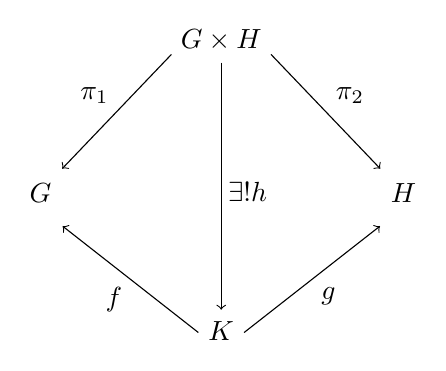
\begin{tikzpicture}[x=0.75pt,y=0.75pt,yscale=-1,xscale=1]
\draw[->]    (289,95) -- (289,214) ;
\draw[->]    (265,91) -- (212.38,146.05) ;
\draw[->]    (313,91) -- (365.62,146.05) ;
\draw[->]    (278,225) -- (212.57,173.73) ;
\draw[->]    (300,225) -- (365.47,173.73) ;
\draw (289,90.6) node [anchor=south] [inner sep=0.75pt]    {$G\times H$};
% Text Node
\draw (289,218.4) node [anchor=north] [inner sep=0.75pt]    {$K$};
% Text Node
\draw (208.5,157.75) node [anchor=east] [inner sep=0.75pt]    {$G$};
% Text Node
\draw (369.5,157.75) node [anchor=west] [inner sep=0.75pt]    {$H$};
% Text Node
\draw (291,157.25) node [anchor=west] [inner sep=0.75pt]    {$\exists !h$};
% Text Node
\draw (236,115.85) node [anchor=south east] [inner sep=0.75pt]    {$\pi _{1}$};
% Text Node
\draw (343,115.85) node [anchor=south west] [inner sep=0.75pt]    {$\pi _{2}$};
% Text Node
\draw (242.5,202.15) node [anchor=north east] [inner sep=0.75pt]    {$f$};
% Text Node
\draw (336,202.15) node [anchor=north west][inner sep=0.75pt]    {$g$};
\end{tikzpicture}
\end{figure}
\begin{proof}
	和之前线性空间中一样,对于$\forall k\in K$,直接取$h(k):=(f(k),g(k))$即可。
\end{proof}
\subsubsection{对于与拓扑空间而言}\label{c3223}
设$X,Y$是两个拓扑空间,$X\times Y$是其乘积拓扑空间,定义映射:
\begin{equation*}
	\begin{aligned}
		\pi_{1} : X\times Y&\longrightarrow X\\
		(x,y)&\longmapsto x
	\end{aligned}
\end{equation*}
\begin{equation*}
	\begin{aligned}
		\pi_{2} : X\times Y&\longrightarrow Y\\
		(x,y)&\longmapsto y
	\end{aligned}
\end{equation*}
\begin{lemma}\label{c3-y1}
	上定义的$\pi_{1}$和$\pi_{2}$是连续映射。
\end{lemma}
\begin{proof}
	只需证明映射$\pi_{1}$是连续映射即可,任取$U\subset_{open}X$,那么其关于$\pi_{1}$的逆像为$\pi_{1}^{-1}(U) = U\times Y$,这是开集。
\end{proof}
\begin{lemma}
	设$X,Y,Z$为仨拓扑空间,$X\times Y$为乘积拓扑空间,对于$\forall f:Z\longrightarrow X\times Y$有:
	\begin{equation*}
		f\text{连续}\iff	\pi_{1}\circ f,\pi_{2}\circ f\text{连续}
	\end{equation*}
\end{lemma}
\begin{proof}
	证明其充分必要即可:
	\begin{enumerate}
		\item[[\lei{$\Rightarrow $}]]:由于$f$是连续映射以及引理\ref{c3-y1}可知$\pi_{1}$和$\pi_{2}$也是连续映射。得证。
		\item[[\lei{$\Leftarrow $}]]:要证:$\forall$开集$W\subset X\times Y,f^{-1}(W)$是开集。只要证$\forall U\subset_{open}X,V\subset_{open}Y,f^{-1}(U\times V)$是开集。事实上:
		\begin{equation*}
			\begin{aligned}
				f^{-1}(U\times V) &= \dkh{z\in Z|f(z)=(\pi_{1}\circ f(z) , \pi_{2}\circ f(z)) \in U\times V}\\
				&=\dkh{z\in Z|\pi_{1}\circ f(z)\in U,\pi_{2}\circ f(z)\in V}\\
				&=(\pi_{1}\circ f)^{-1}(U)\cap(\pi_{2}\circ f)^{-1}(V)
			\end{aligned}
		\end{equation*}
		这是开集,因此得证。
	\end{enumerate}
\end{proof}
\subsubsection{范畴与范畴的乘积}
\begin{definition}[范畴]
	一个\gn{范畴}(\gn{category})$\mathcal{C}$是指下面的数据:
	\begin{enumerate}
		\item 一些被称为\gn{对象}(\gn{object})的东西所组成的集合$\mathcal{O}b\mathcal{(C)}$。
		\item 一些被称为\gn{态射}(\gn{morphism})的东西所组成的集合$\mathcal{H}om\mathcal{(C)}$。
		\item 映射:\begin{equation*}
			\begin{aligned}
				s(\gn{source}):\mathcal{H}om\mathcal{(C)}&\longrightarrow \mathcal{O}b\mathcal{(C)}\\
				f\longmapsto s(f)
			\end{aligned}
		\end{equation*}
		\begin{equation*}
			\begin{aligned}
				t(\gn{target}):\mathcal{H}om\mathcal{(C)}&\longrightarrow \mathcal{O}b\mathcal{(C)}\\
				f\longmapsto t(f)
			\end{aligned}
		\end{equation*}
	
	
	对于$\forall f\in \mathcal{H}om\mathcal{(C)},s(f) = X,t(f)=Y$,记$f:X\longrightarrow Y$,记$\hom_{\mathcal{C}}(X,Y) := \dkh{f\in \mathcal{H}om\mathcal{(C)}|s(f) = X,t(f) = Y}$
	\item 态射的\gn{复合$\circ$}(\gn{composition}):
	\begin{equation*}
		\begin{aligned}
			\circ : \hom(X,Y)\times \hom(Y,Z)&\longrightarrow  \hom(X,Z)\\
			(f,g)&\longmapsto g\circ f
		\end{aligned}
	\end{equation*}
	\end{enumerate}
	满足下列运算律:\begin{enumerate}
		\item \lei{结合律}:$\forall  X,Y,Z,W$满足关系:

\begin{center}
\tikzset{every picture/.style={line width=0.5pt}}
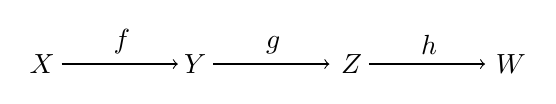
\begin{tikzpicture}[x=0.75pt,y=0.75pt,yscale=-1,xscale=1]
\draw[->]    (169,147) -- (225,147) ;
\draw[->]     (242,147) -- (298,147) ;
\draw[->]     (317,147) -- (373,147) ;
\draw (167,147) node [anchor=east] [inner sep=0.75pt]    {$X$};
\draw (240,147) node [anchor=east] [inner sep=0.75pt]    {$Y$};
\draw (315,147) node [anchor=east] [inner sep=0.75pt]    {$Z$};
\draw (377,147) node [anchor=west] [inner sep=0.75pt]    {$W$};
\draw (198,143.6) node [anchor=south] [inner sep=0.75pt]    {$f$};
\draw (271,143.6) node [anchor=south] [inner sep=0.75pt]    {$g$};
\draw (346,143.6) node [anchor=south] [inner sep=0.75pt]    {$h$};
\end{tikzpicture}
\end{center}
有:
$$(h\circ g)\circ f = h\circ (g\circ f)$$
		\item \lei{恒等态射}:$\forall X\in \mathcal{O}b(\mathcal{C}),\exists \gn{1_{X}}:X\longrightarrow X,\st \forall f:X\longrightarrow Y;g:Z\longrightarrow X$有$f\circ 1_{X} = f,1_{X}\circ g = g$,并且恒等态射是唯一的。
	\end{enumerate}
\end{definition}
\begin{definition}[态射的同构]
	设$\mathcal{C}$是一个范畴,$X,Y$为$\mathcal(C)$中的两个对象,如果$\exists $两个态射$f:X\longrightarrow Y,g:Y\longrightarrow X\st f\circ g=1_{Y},g\circ f=1_{X}$,那么称$X$与$Y$是\gn{同构的}。
\end{definition}
\begin{example}[域$\mathbb{K}$上的线性空间范畴]
	节\ref{c3221}中所叙述的Vect$_{\mathbb{K}}$是\gn{域$\mathbb{K}$上的线性空间范畴}。
\end{example}
\begin{example}[群范畴]
	节\ref{c3222}中所叙述的Grp是\gn{群范畴}。
\end{example}
\begin{example}[拓扑空间范畴]
	节\ref{c3223}中所叙述的Top是\gn{拓扑空间范畴}。
\end{example}
\begin{definition}[范畴乘积]
	设$\mathcal{C}$是一个范畴,$x_{1},X_{2}\in \mathcal{O}b{\mathcal{C}}$,$X_{1}$与$X_{2}$的\gn{乘积}是指如下数据:
	\begin{enumerate}
		\item $Y\in \mathcal{O}b(\mathcal{(C)})$,其中记$Y = X_{1}\times X_{2}$
		\item $\pi_{1}:Y\longrightarrow X_{1},\pi_{2}:Y\longrightarrow X_{2}$,满足以下Universal Property:
		
		$\exists Z\in \mathcal{O}b(\mathcal{C})$以及$f:Z\longrightarrow X_{1},g:Z\longrightarrow X_{2},\exists  !$态射$h:Z\longrightarrow Y,\st $下列图表交换:

	\begin{center}
\tikzset{every picture/.style={line width=0.75pt}}
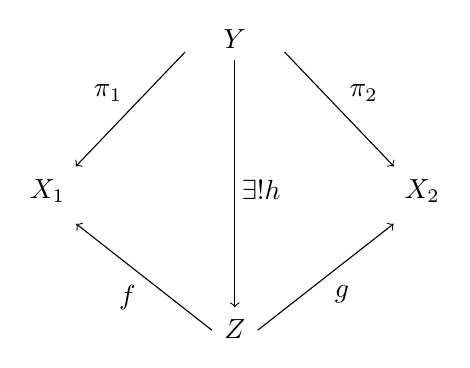
\begin{tikzpicture}[x=0.75pt,y=0.75pt,yscale=-1,xscale=1]
\draw[->]    (289,95) -- (289,214) ;
\draw[->]    (265,91) -- (212.38,146.05) ;
\draw[->]    (313,91) -- (365.62,146.05) ;
\draw[->]    (278,225) -- (212.57,173.73) ;
\draw[->]    (300,225) -- (365.47,173.73) ;
\draw (289,90.6) node [anchor=south] [inner sep=0.75pt]    {$Y$};
% Text Node
\draw (289,218.4) node [anchor=north] [inner sep=0.75pt]    {$Z$};
% Text Node
\draw (208.5,157.75) node [anchor=east] [inner sep=0.75pt]    {$X_{1}$};
% Text Node
\draw (369.5,157.75) node [anchor=west] [inner sep=0.75pt]    {$X_{2}$};
% Text Node
\draw (291,157.25) node [anchor=west] [inner sep=0.75pt]    {$\exists !h$};
% Text Node
\draw (236,115.85) node [anchor=south east] [inner sep=0.75pt]    {$\pi _{1}$};
% Text Node
\draw (343,115.85) node [anchor=south west] [inner sep=0.75pt]    {$\pi _{2}$};
% Text Node
\draw (242.5,202.15) node [anchor=north east] [inner sep=0.75pt]    {$f$};
% Text Node
\draw (336,202.15) node [anchor=north west][inner sep=0.75pt]    {$g$};
\end{tikzpicture}
	\end{center}
		\end{enumerate}
\end{definition}
\begin{note}
如果$X_{1}$与$X_{2}$的乘积存在,则其在同构下唯一。假设$(Y',\pi_{1}':Y'\longrightarrow X_{1},\pi_{2}':Y'\longrightarrow X_{2})$也满足以上	Universal Property:
\begin{center}
\tikzset{every picture/.style={line width=0.75pt}}
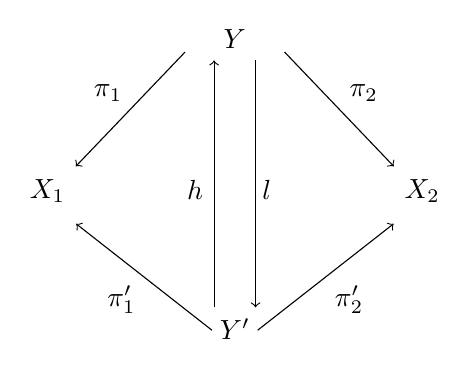
\begin{tikzpicture}[x=0.75pt,y=0.75pt,yscale=-1,xscale=1]
\draw[->]    (279,214) -- (279,95) ;
\draw[->]    (299,95) -- (299,214) ;
\draw[->]    (265,91) -- (212.38,146.05) ;
\draw[->]    (313,91) -- (365.62,146.05) ;
\draw[->]    (278,225) -- (212.57,173.73) ;
\draw[->]    (300,225) -- (365.47,173.73) ;
\draw (289,90.6) node [anchor=south] [inner sep=0.75pt]    {$Y$};
% Text Node
\draw (289,218.4) node [anchor=north] [inner sep=0.75pt]    {$Y'$};
% Text Node
\draw (208.5,157.75) node [anchor=east] [inner sep=0.75pt]    {$X_{1}$};
% Text Node
\draw (369.5,157.75) node [anchor=west] [inner sep=0.75pt]    {$X_{2}$};
% Text Node
\draw (301,157.25) node [anchor=west] [inner sep=0.75pt]    {$l$};

\draw (275,157.25) node [anchor=east] [inner sep=0.75pt]    {$h$};
% Text Node
\draw (236,115.85) node [anchor=south east] [inner sep=0.75pt]    {$\pi _{1}$};
% Text Node
\draw (343,115.85) node [anchor=south west] [inner sep=0.75pt]    {$\pi _{2}$};
% Text Node
\draw (242.5,202.15) node [anchor=north east] [inner sep=0.75pt]    {$\pi_{1}'$};
% Text Node
\draw (336,202.15) node [anchor=north west][inner sep=0.75pt]    {$\pi_{2}'$};
\end{tikzpicture}
	\end{center}

那么$h\circ h:Y'\longrightarrow Y'$
\begin{center}
\tikzset{every picture/.style={line width=0.75pt}}
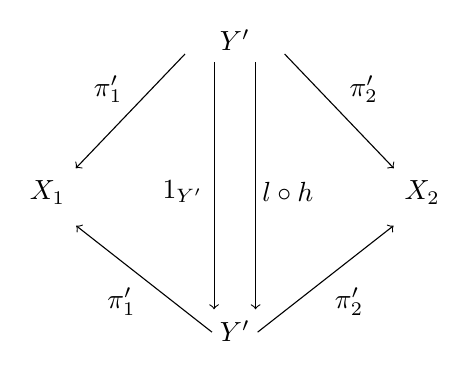
\begin{tikzpicture}[x=0.75pt,y=0.75pt,yscale=-1,xscale=1]
\draw[->]    (279,95) -- (279,214) ;
\draw[->]    (299,95) -- (299,214) ;
\draw[->]    (265,91) -- (212.38,146.05) ;
\draw[->]    (313,91) -- (365.62,146.05) ;
\draw[->]    (278,225) -- (212.57,173.73) ;
\draw[->]    (300,225) -- (365.47,173.73) ;
\draw (289,90.6) node [anchor=south] [inner sep=0.75pt]    {$Y'$};
% Text Node
\draw (289,218.4) node [anchor=north] [inner sep=0.75pt]    {$Y'$};
% Text Node
\draw (208.5,157.75) node [anchor=east] [inner sep=0.75pt]    {$X_{1}$};
% Text Node
\draw (369.5,157.75) node [anchor=west] [inner sep=0.75pt]    {$X_{2}$};
% Text Node
\draw (301,157.25) node [anchor=west] [inner sep=0.75pt]    {$l\circ h$};

\draw (275,157.25) node [anchor=east] [inner sep=0.75pt]    {$1_{Y'}$};
% Text Node
\draw (236,115.85) node [anchor=south east] [inner sep=0.75pt]    {$\pi _{1}'$};
% Text Node
\draw (343,115.85) node [anchor=south west] [inner sep=0.75pt]    {$\pi _{2}'$};
% Text Node
\draw (242.5,202.15) node [anchor=north east] [inner sep=0.75pt]    {$\pi_{1}'$};
% Text Node
\draw (336,202.15) node [anchor=north west][inner sep=0.75pt]    {$\pi_{2}'$};
\end{tikzpicture}
	\end{center}
	
根据图很容易得到:
\begin{equation*}
	\pi_{1}'\circ (l\circ h) = (\pi_{1}'\circ l)\circ h = \pi_{1}\circ h = \pi_{1}'
\end{equation*}
就得到:
\begin{equation*}
	1_{Y'} = l\circ h
\end{equation*}
类似可以得到:
\begin{equation*}
	h\circ l = 1_{Y} 
\end{equation*}
因此就是说$Y'$和$Y$是同构的。
\end{note}
\begin{conclusion}
	对于拓扑空间$X_{1},X_{2}$,令$X_{1}\times X_{2}$为其乘积拓扑空间,我们已经证明$(X_{1}\times X_{2},\pi_{1},\pi_{2})$为$X_{1},X_{2}$在拓扑空间中的乘积。
\end{conclusion}
\subsection{乘积拓扑与紧性}
\begin{lemma}
	设$X$为一个拓扑空间,设$\tpj$为$X$的一个拓扑基,则:
	\begin{equation*}
		X\text{紧}\iff \forall\text{一族}\dkh{U_{\alpha}}_{\alpha \in I}\subset\tpj,\dkh{U_{\alpha}}_{\alpha \in I}\text{覆盖}X\text{,则}\dkh{U_{\alpha}}_{\alpha\in  I}\text{存在有限子覆盖}
	\end{equation*}
\end{lemma}
\begin{proof}
	必要性是显然的,下只需证明充分性。
	
	任取$X$的开覆盖$\dkh{V_{\alpha}}_{\alpha\in J}$,使得:
	\begin{equation*}
		\dabing_{\alpha\in J}V_{\alpha} = X
	\end{equation*}
而由于$\tpj$为$X$的一个拓扑基,就有:$V_{\alpha} = \dabing_{U_{\alpha i}\in \tpj}U_{\alpha i}$,根据条件。就知道$\exists U_{\alpha_{1}i_{1}},U_{\alpha_{2}i_{2}},\cdots,U_{\alpha_{n}i_{n}}\in \dkh{U_{\alpha i}},\st \dabing_{j=1}^{n}U_{\alpha_{j}i_{j}} = X$,其中$U_{\alpha_{j}i_{j}}\subset V_{\alpha_{j}}$,因此$\dabing_{j=1}^{n}V_{j} = X$。
\end{proof}

\begin{proposition}[紧集的直积集是紧集]
	设$X,Y$是紧集,那么$X\times Y$也是紧集。
\end{proposition}
\begin{proof}
	任取$\dkh{U_{\alpha}\times V_{\alpha}}_{\alpha\in I}$为$X\times Y$的一组开覆盖,任取$x\in X$,作为单点集$\dkh{x}$与$X$的乘积拓扑空间$\dkh{x}\times Y\cong Y$,而且由于$Y$是紧集得知$\dkh{x}\times Y$也是紧集。
	
	那么任取$\dkh{U_{\alpha}\times V_{\alpha}}_{\alpha\in I}$是$\dkh{x}\times Y$的开覆盖,那么其必存在有限子覆盖$\dkh{U_{\alpha}^{x}\times V_{\alpha}^{x}}_{\alpha =1}^{n_{x}}$,令:
	\begin{equation*}
		U^{x} = \dajiao_{j = 1}^{n_{x}} U_{j}^{x}  \subset_{open} X
	\end{equation*}
	
	那么$$\dabing_{x\in X}U^{x}= X$$又由于$X$是紧集,因此$\exists x_{1} , x_{2},\cdots , x_{n} \st X\subset \dabing_{i=1}^{n}U^{x_{i}}$,那么再对$Y$做类似的事情,就得到一列乘积集合$\dkh{\dkh{U_{j}^{x_{i}}\times V_{j}^{x_{i}}}_{j = 1}^{n_{x_{i}}}}_{i = 1}^{m}$,并且每一行$U^{x_{i}}\times Y\subset \dabing_{j=1}^{n_{x_{i}}}U_{j}^{x_{i}}\times V_{j}^{x_{i}}$,满足:
	\begin{equation*}
		X\times Y\subset \dabing_{i=1}^{m}\dabing_{j=1}^{n_{x_{i}}}U_{j}^{x_{i}}\times V_{j}^{x_{i}}
	\end{equation*}
	右侧乘积集合的个数是有限的,因此$X\times Y$是紧集。
\end{proof}

\subsection{紧性为拓扑不变性}
\begin{proposition}[紧性是一个拓扑不变量]\label{c3-m4}
	设$	X$是紧集,$f:X\longrightarrow Y$是连续映射,那么$f(X)$也是紧集。
\end{proposition}
\begin{note}
本命题的意思是\cukai{紧性在连续映射的作用下被保持}。也就是说,对于两个同胚的拓扑空间而言,这两个拓扑空间同具有紧性或者同不具有紧性。\lei{紧性是一个拓扑不变量!}
\end{note}
\begin{proof}
	对于$\forall f(X)$的一组开覆盖$\dkh{U_{\alpha}}_{\alpha\in I},U_{\alpha}\subset_{open}Y$,那么$\dkh{f^{-1}(U_{\alpha})}_{\alpha\in I}$为$X$的一组开覆盖。由于$X$是紧集,因此$\exists \alpha_{1},\alpha_{2},\cdots,\alpha_{n}, \st X\subset\dabing_{i = 1}^{n}f^{-1}(U_{\alpha_{i}})$,即:$f(X)\subset\dabing_{i=1}^{n}U_{\alpha_{i}}$。
\end{proof}
\begin{corollary}
	紧空间上的连续实值函数有界,并可以取到最值。
\end{corollary}
\begin{proof}
	设$X$是紧集,$f:X\longrightarrow \mathbb{R}$是连续映射,根据上命题\ref{c3-m4}可知$f(X)$是紧集,根据定理\ref{c3-t2}可知$f(X)$是有界闭集,下设$S = \sup f(X),s=\inf f(X)$,由于$f(X)$是闭集,集合的上确界和下确界都可在集合中取到。因此$S,s\in f(X)$。
\end{proof}
\subsection{更多的紧性}
\begin{definition}[极限点紧性]
	设$X$为拓扑空间,如果$X$中的任意无限子集都有极限点,就称$X$是\gn{极限点紧}\footnote{By Munkers : 在拓扑学早期,这种紧性被称为\gn{紧致性}。如同我们在数学分析中证明的一样,不过在这里我们需要区分紧支集、紧致性、紧性、列紧性。}的。
\end{definition}
\begin{proposition}
	紧性蕴含极限点紧性。
\end{proposition}
\begin{proof}
	设$ X$是紧集,任取无限集合$A\subset X$,假设$A$没有极限点,即:
	\begin{equation*}
		\forall x\in X ,\exists U_{x}\subset_{open}X,\st (U_{x}\chadiao\dkh{x})\cap A = \emptyset
 	\end{equation*}
 	即$U_{x}$中最多只有$A$中的一个点。另一方面,由于$X$的紧性可以知道,任取$X$的一个开覆盖$\dkh{U_{x}}_{x\in X}\supset X$,总存在有限子覆盖$\dkh{U_{x_{i}}}_{i=1}^{n}$使得$$ \dabing_{i=1}^{n}U_{x_{i}} = X\supset A$$
 	而上式左侧是有限并,每一个集合中做多只有$A$的一个点,所以左侧最多只有$A$集合中的$n$个点;右侧包含无限子集$A$,因此有$A$中的无限多个点,这就矛盾!
\end{proof}
\begin{example}[极限点紧性与紧性不等价]
	正整数集$\mathbb{Z}_{+} = \dkh{1,2,3,\cdots,n,\cdots}$上赋予离散拓扑;$Y = \dkh{0,1}$上赋予平凡拓扑,其直积集$\mathbb{Z}_{+}\times Y$赋予乘积拓扑的条件下是极限点紧集,而非紧集。
	\begin{proof}
		对于$\forall \emptyset \neq A\subset \mathbb{Z}_{+}\times Y$,若$(n,1)\in A$,那么$(n,1)$是$A$的极限点。因此之当然是极限点紧集。但是其并非紧集,比如对于一组开集族$\dkh{\dkh{n}\times Y}_{n=1,2,\cdots}$显然是$\mathbb{Z}_{+}\times Y$的一组开覆盖,但是其并没有一个有限子覆盖。
		
%		但是对于$\mathbb{Z}_{+}\times Y$的一组拓扑基为$\dkh{n}\times Y,n=1,2,\cdots$,则$\forall U\subset_{open}\mathbb{Z}_{+}\times Y,(n,0)\in U$
	\end{proof}\end{example}
	\begin{definition}[列紧性]
		设$X$为一个拓扑空间,如果对于$X$中的任何一个无限点列$\dkh{x_{n}}_{n=1}^{\infty}$都有收敛子列,就称$X$是一个\gn{列紧集}。
	\end{definition}
\begin{proposition}
	列紧性蕴含极限点紧性。
\end{proposition}
\begin{proof}
	对于列紧集$X$取任何无限集合$ A\subset X$,任取$\dkh{x_{n}}_{n=1}^{\infty}$是$A$的一个点列,$x_{n}$互不相同。则$\dkh{x_{n}}_{n=1}^{\infty}$有收敛子列$\dkh{x_{n_{k}}},\st x_{n_{k}}\to x_{0}(k\to +\infty)$,因此$x_{0}$为$A$的极限点,因此$X$是极限点紧集。
\end{proof}
\begin{example}[列紧性与极限点紧性不等价]
	对于实数集$\mathbb{R}$,赋予\gn{右拓扑}:$\tp = \dkh{(a,+\infty)|a\in \mathbb{R}}\cup\emptyset$,明显$(\mathbb{R},\tp)$是极限点紧集\footnote{这是因为:任取$\emptyset\neq A\subset\mathbb{R}$。设$x_{0}\in A$,则$x_{0}-1$是$A$的一个极限点,这是因为此时$\forall U\subset_{open}\mathbb{R}$$U$可以表示为$(x,+\infty),x<x_{0}-1$,此时有:
	\begin{equation*}
		x_{0}\in (U\chadiao\dkh{x_{0}-1})\cap A \neq \emptyset
	\end{equation*}}。但是$(\mathbb{R},\tp)$并非列紧集。
	\begin{proof}
		直接取点列为$x_{n} = -n,n\in \mathbb{N}$,假设其有收敛子列$\dkh{x_{n_{k}}}_{k=1}^{\infty},\st x_{n_{k}}\to x_{0}(k\to +\infty)$,即:
		\begin{equation*}
			\forall U\subset_{open}\mathbb{R}(x_{0}\in U),\exists N,\st \forall k>N,x_{n_{k}}\in U
		\end{equation*}
		但是实际上$\forall U\subset_{open}\mathbb{R}$,都可以写成$U=(a,+\infty),a<x_{0}$,那么必然存在$M,\st \forall k>M,x_{n_{k}}<a,x_{n_{k}}\notin U$。
	\end{proof}
\end{example}
\begin{theorem}
	在度量空间中,紧性、极限点紧性、列紧性互相等价。
\end{theorem}
%第四章	
\chapter{连通性}
在这一节,我们要再引入另一个拓扑不变量,即连通性,连通性在复分析中有很高的出场率。
\section{连通性与连通分支}
\subsection{连通性}
为了考虑一个集合的连通性,我们先来考虑一集合不连通是一个什么情况。
\begin{definition}[连通性]
	设$X$是一个拓扑空间,如果$X$可以被分解为两个非空开集的直和,就称$X$是\gn{不连通}的。即:
	\begin{equation*}
		X=  U\sqcup V,U\subset_{open}X,V\subset_{open}X;U,V\neq \emptyset
	\end{equation*}
\end{definition}
\begin{note}
	由此可以看出,我们说一个集合是\tl{不连通}的,是可以把它分解成两个独立的部分,这两个部分是既开又闭,因此每一个部分中的点、极限点都只被限定在这个部分之中,任何一个部分的点从该部分往任何地方跑,都不可以直接到达另一个部分。
	\begin{figure}[h]
		\centering
\tikzset{every picture/.style={line width=0.75pt}} %set default line width to 0.75pt        

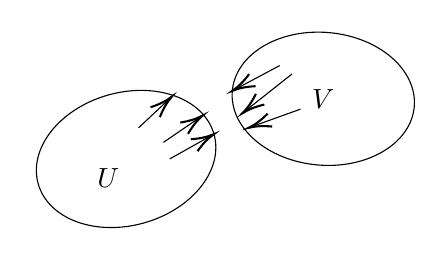
\begin{tikzpicture}[x=0.75pt,y=0.75pt,yscale=-1,xscale=1]
%uncomment if require: \path (0,300); %set diagram left start at 0, and has height of 300

%Shape: Ellipse [id:dp8624803269432] 
\draw   (101.66,146.98) .. controls (96.85,129.97) and (111.9,110.83) .. (135.29,104.21) .. controls (158.67,97.59) and (181.53,106.01) .. (186.34,123.02) .. controls (191.15,140.03) and (176.1,159.17) .. (152.71,165.79) .. controls (129.33,172.41) and (106.47,163.99) .. (101.66,146.98) -- cycle ;
%Shape: Ellipse [id:dp6936201842442715] 
\draw   (195.17,102.18) .. controls (196.7,84.57) and (217.57,72.01) .. (241.78,74.12) .. controls (265.99,76.23) and (284.37,92.21) .. (282.83,109.82) .. controls (281.3,127.43) and (260.43,139.99) .. (236.22,137.88) .. controls (212.01,135.77) and (193.63,119.79) .. (195.17,102.18) -- cycle ;
%Straight Lines [id:da582018709351726] 
\draw    (150,120) -- (164.54,106.37) ;
\draw [shift={(166,105)}, rotate = 136.85] [color={rgb, 255:red, 0; green, 0; blue, 0 }  ][line width=0.75]    (10.93,-3.29) .. controls (6.95,-1.4) and (3.31,-0.3) .. (0,0) .. controls (3.31,0.3) and (6.95,1.4) .. (10.93,3.29)   ;
%Straight Lines [id:da22908013955818896] 
\draw    (162,127) -- (179.35,115.13) ;
\draw [shift={(181,114)}, rotate = 145.62] [color={rgb, 255:red, 0; green, 0; blue, 0 }  ][line width=0.75]    (10.93,-3.29) .. controls (6.95,-1.4) and (3.31,-0.3) .. (0,0) .. controls (3.31,0.3) and (6.95,1.4) .. (10.93,3.29)   ;
%Straight Lines [id:da4126636864109632] 
\draw    (165,135) -- (184.59,124) ;
\draw [shift={(186.34,123.02)}, rotate = 150.69] [color={rgb, 255:red, 0; green, 0; blue, 0 }  ][line width=0.75]    (10.93,-3.29) .. controls (6.95,-1.4) and (3.31,-0.3) .. (0,0) .. controls (3.31,0.3) and (6.95,1.4) .. (10.93,3.29)   ;
%Straight Lines [id:da904012699639372] 
\draw    (224,94) -- (201.57,111.76) ;
\draw [shift={(200,113)}, rotate = 321.63] [color={rgb, 255:red, 0; green, 0; blue, 0 }  ][line width=0.75]    (10.93,-3.29) .. controls (6.95,-1.4) and (3.31,-0.3) .. (0,0) .. controls (3.31,0.3) and (6.95,1.4) .. (10.93,3.29)   ;
%Straight Lines [id:da8244179446110391] 
\draw    (228,111) -- (204.88,119.32) ;
\draw [shift={(203,120)}, rotate = 340.2] [color={rgb, 255:red, 0; green, 0; blue, 0 }  ][line width=0.75]    (10.93,-3.29) .. controls (6.95,-1.4) and (3.31,-0.3) .. (0,0) .. controls (3.31,0.3) and (6.95,1.4) .. (10.93,3.29)   ;
%Straight Lines [id:da789966203802531] 
\draw    (218,90) -- (196.93,101.24) ;
\draw [shift={(195.17,102.18)}, rotate = 331.92] [color={rgb, 255:red, 0; green, 0; blue, 0 }  ][line width=0.75]    (10.93,-3.29) .. controls (6.95,-1.4) and (3.31,-0.3) .. (0,0) .. controls (3.31,0.3) and (6.95,1.4) .. (10.93,3.29)   ;
\draw (142,138.4) node [anchor=north east] [inner sep=0.75pt]    {$U$};
\draw (239,106) node    {$V$};
\end{tikzpicture}
\caption{集合$X=U\sqcup V$是不连通的}
	\end{figure}
\end{note}
\begin{example}[$\mathbb{R}$中不是不连通的例子]
	设集合$X = [0,2]$赋予之欧氏拓扑空间的子空间拓扑,$X$是\tl{不是不连通的},这是因为$X= [0,2] = [0,1)\sqcup [1,2]$,其中 比如$[0,1)$并非是子空间意义下的闭集(从而$[1,2]$也不是子空间意义下的开集)。对于其他的分解也都是这种情况。
\end{example}

\begin{example}[$\mathbb{R}$中不连通的例子]
	设集合$X=[0,1)\cup(1,2]$,那么$X = ((-1,1)\cap X)\sqcup((1,3)\cap X)$,在子空间拓扑下两侧集合都是开集和闭集,因此$X$在子空间拓扑意义下是不连通的。
\end{example}
\begin{example}[圆扣掉两个点就不连通了]
	设$X = S^{1}\chadiao\dkh{P,Q} = (\dkh{x<0}\cap X)\sqcup(\dkh{x>0}\cap X)$,因此其是不连通的。\end{example}
	\begin{figure}[h]
		\centering


\tikzset{every picture/.style={line width=0.75pt}} %set default line width to 0.75pt        

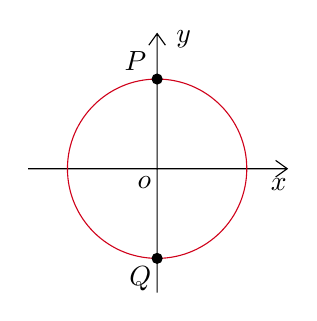
\begin{tikzpicture}[x=0.75pt,y=0.75pt,yscale=-1,xscale=1,scale=0.8]
%uncomment if require: \path (0,300); %set diagram left start at 0, and has height of 300

%Shape: Axis 2D [id:dp9727015375843877] 
\draw  (115.38,169) -- (271.38,169)(193,87.61) -- (193,243.61) (264.38,164) -- (271.38,169) -- (264.38,174) (188,94.61) -- (193,87.61) -- (198,94.61)  ;
%Shape: Circle [id:dp7282422916468221] 
\draw  [color={rgb, 255:red, 208; green, 2; blue, 27 }  ,draw opacity=1 ] (139,169) .. controls (139,139.18) and (163.18,115) .. (193,115) .. controls (222.82,115) and (247,139.18) .. (247,169) .. controls (247,198.82) and (222.82,223) .. (193,223) .. controls (163.18,223) and (139,198.82) .. (139,169) -- cycle ;
%Shape: Circle [id:dp9329032514915467] 
\draw  [fill={rgb, 255:red, 0; green, 0; blue, 0 }  ,fill opacity=1 ] (190,115) .. controls (190,113.34) and (191.34,112) .. (193,112) .. controls (194.66,112) and (196,113.34) .. (196,115) .. controls (196,116.66) and (194.66,118) .. (193,118) .. controls (191.34,118) and (190,116.66) .. (190,115) -- cycle ;
%Shape: Circle [id:dp8971655931886666] 
\draw  [fill={rgb, 255:red, 0; green, 0; blue, 0 }  ,fill opacity=1 ] (190,223) .. controls (190,221.34) and (191.34,220) .. (193,220) .. controls (194.66,220) and (196,221.34) .. (196,223) .. controls (196,224.66) and (194.66,226) .. (193,226) .. controls (191.34,226) and (190,224.66) .. (190,223) -- cycle ;
\draw (188,111.6) node [anchor=south east] [inner sep=0.75pt]    {$P$};
% Text Node
\draw (191,226.4) node [anchor=north east] [inner sep=0.75pt]    {$Q$};
% Text Node
\draw (191,172.4) node [anchor=north east] [inner sep=0.75pt]    {$o$};
% Text Node
\draw (260,173.4) node [anchor=north west][inner sep=0.75pt]    {$x$};
\draw (203,84.4) node [anchor=north west][inner sep=0.75pt]    {$y$};
\end{tikzpicture}\caption{例4.3中的$X = S^{1}\chadiao\dkh{P,Q}$}
	\end{figure}
\begin{definition}[连通性]
	设$X$为一个拓扑空间,如果$X = U\sqcup V$,其中$U,V\subset_{open }X$,则$U,V$中至少有一个为空集。则称$X$是\gn{连通}的。
\end{definition}

\begin{proposition}
	
	设$X$是一个拓扑空间,则下列三条等价:
	\begin{enumerate}
	\item $X$连通。
	\item $X$中既开又闭之集合只能为$\emptyset, X$。
	\item 不存在一个连续的满射$f:X\longrightarrow Y$。其中$Y$赋予离散拓扑结构,且$Y$中元素之个数不少于2。	
	\end{enumerate}
	\end{proposition}
	\begin{proof}
		该命题给予了连通性的几个等价叙述,下循环证之:
		\begin{enumerate}
			\item[[\lei{1}$\Rightarrow\lei{2}$]]: 若$U\subset_{open,closed}X$则$X\chadiao U\subset_{open,closed}$,由于$X = U\sqcup (X\chadiao U)$,且$X$是连通的,就说明$U$和$X\chadiao U$中至少有一个为空集。得证。
			\item[[\lei{2}$\Rightarrow\lei{3}$]]: 假设存在连续满射:
			\begin{equation*}
				f:X\longrightarrow Y
			\end{equation*}
			满足赋予$Y$离散拓扑,且$|Y| \geq 2$,那么任取$y\in Y$,在离散拓扑意义下$y$既为开集又为闭集,由于$f$是连续映射,则$f^{-1}(y)$既为开集又为闭集,如果$f^{-1}(y)=X$,那么$|Y| = 1$显然不成立,则$f^{-1}(y)\neq X$,因此$f^{-1}(y)=\emptyset$,这又与$f$为满射矛盾。
			\item[[\lei{3}$\Rightarrow\lei{1}$]]: 假设$X = U\sqcup V;U,V\subset_{open}X ;U,V\neq \emptyset$,令:
			\begin{equation*}
				\begin{aligned}
					f:X&\longrightarrow\dkh{0,1}\\
					x&\longmapsto f(x) = \left\{ \begin{aligned}
					&1,x\in U\\
					&0,x\in V
					\end{aligned} \right.
				\end{aligned}
			\end{equation*}
			那么就有$f^{-1}(1) = U,f^{-1}(0) = V$,与$f$为一个连续满射,与\lei{3}矛盾。
		\end{enumerate}
	\end{proof}





在数学分析之中,我们常常在$\mathbb{R}$上研究问题,因此下面我们考虑一些$\mathbb{R}$上的连通性的例子。

\begin{proposition}
	$\mathbb{R}$在欧氏拓扑意义下是连通的。
\end{proposition}
\begin{proof}
	假设$\mathbb{R}$不连通,即:
	\begin{equation*}
		\exists U\subset_{open,closed}\mathbb{R},U\neq \emptyset,\mathbb{R}
	\end{equation*}
	则$\exists x_{1}\in \mathbb{R}\chadiao U,\exists x_{2}\in U$,不妨设$x_{1}<x_{2}$,考虑集合$S = \dkh{x\in \mathbb{R}|x\geq x_{1},[x_{1},x_{2}]\subset \mathbb{R}\chadiao U}$。
	
	\begin{figure}[h]
		\centering
		

\tikzset{every picture/.style={line width=0.75pt}} %set default line width to 0.75pt        

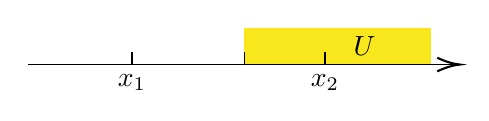
\begin{tikzpicture}[x=0.75pt,y=0.75pt,yscale=-1,xscale=1]
%uncomment if require: \path (0,300); %set diagram left start at 0, and has height of 300

%Shape: Rectangle [id:dp25984372613253615] 
\draw  [color={rgb, 255:red, 248; green, 231; blue, 28 }  ,draw opacity=1 ][fill={rgb, 255:red, 248; green, 231; blue, 28 }  ,fill opacity=1 ] (204,94.5) -- (294,94.5) -- (294,112) -- (204,112) -- cycle ;
%Straight Lines [id:da9856667544417632] 
\draw    (100,112) -- (306,112) ;
\draw [shift={(308,112)}, rotate = 180] [color={rgb, 255:red, 0; green, 0; blue, 0 }  ][line width=0.75]    (10.93,-3.29) .. controls (6.95,-1.4) and (3.31,-0.3) .. (0,0) .. controls (3.31,0.3) and (6.95,1.4) .. (10.93,3.29)   ;
%Straight Lines [id:da812503550526777] 
\draw    (204,106) -- (204,112) ;
%Straight Lines [id:da4930812729568812] 
\draw    (150,106) -- (150,112) ;
%Straight Lines [id:da5135502597081416] 
\draw    (243,106) -- (243,112) ;

% Text Node
\draw (150,115.4) node [anchor=north] [inner sep=0.75pt]    {$x_{1}$};
% Text Node
\draw (243,115.4) node [anchor=north] [inner sep=0.75pt]    {$x_{2}$};
% Text Node
\draw (255.5,103) node [anchor=west] [inner sep=0.75pt]    {$U$};


\end{tikzpicture}
\caption{命题4.2之区间关系图}
	\end{figure}
	首先\tl{$ x_{1}\in S\neq \emptyset$},并且\tl{$S$上有界}($x_{2}$就是$S$的一个上界,这是因为$x_{2}\in U,$则$[x_{1},x_{2}]\nsubseteq \mathbb{R}\chadiao U,\forall y>x_{2},[x_{1},y]\nsubseteq\mathbb{R}\chadiao U$,这就说明$x_{2}$是上界),那么由\lei{确界原理}可知$S$有上确界,记之为$s = \sup S$。那么:
	\begin{enumerate}
		\item $s\in U$,由于$U$是开集,那么$\exists \delta>0,(s-\delta,s+\delta)\subset U,\st s-\dfrac{\delta}{2}$为$S$的一个上界,与$s$是上确界矛盾。
		\item $s\notin U$,由于$\mathbb{R}\chadiao U$为开集,因此$\exists \delta>0,(s-\delta,s+\delta)\subset \mathbb{R}\chadiao U$因此必然$\tl{\exists s_{1}\in S}, s-\delta<s_{1}<s,\tl{\st [x_{1},s_{1}]\subset\mathbb{R}\chadiao U}$,那么就有$[x_{1},s+\dfrac{\delta}{2}]\subset \mathbb{R}\chadiao U$,又与$s$为上确界矛盾。
	\end{enumerate}
	综上,$s$不能为上确界,因此假设有误,归谬。
\end{proof}
\begin{definition}[连通性]
	设$X$为拓扑空间,$Y\subset X$,若$Y$在$X$的子空间拓扑意义下连通,则称$Y$是连通的。
\end{definition}
\begin{proposition}
	$X\subset \mathbb{R}$是连通的$\iff X$为一个区间。
\end{proposition}
\begin{proof}
	命题的必要性是与上命题同理的,下证充分性:
	
	反设$X$并非一个区间,那么就$\exists a<b\in X,\st \exists x_{0}\in \mathbb{R},a<x_{0}<b$,这样定义两个集合:
	\begin{equation*}
		a\in U = (-\infty, x_{0})\cap X\neq \emptyset
	\end{equation*}
	\begin{equation*}
	b\in 	V = (x_{0},+\infty)\cap X\neq \emptyset
	\end{equation*}
	
	\begin{figure}[h]
		\centering


\tikzset{every picture/.style={line width=0.75pt}} %set default line width to 0.75pt        

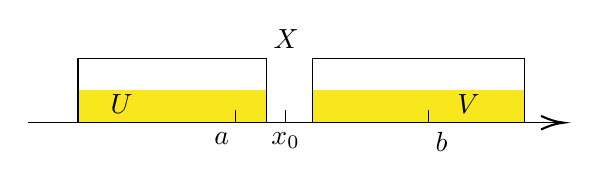
\begin{tikzpicture}[x=0.75pt,y=0.75pt,yscale=-1,xscale=1]
%uncomment if require: \path (0,300); %set diagram left start at 0, and has height of 300

%Shape: Rectangle [id:dp1843188710301753] 
\draw  [color={rgb, 255:red, 248; green, 231; blue, 28 }  ,draw opacity=1 ][fill={rgb, 255:red, 248; green, 231; blue, 28 }  ,fill opacity=1 ] (207,116.5) -- (309,116.5) -- (309,132) -- (207,132) -- cycle ;
%Straight Lines [id:da34892541955377654] 
\draw    (170,126) -- (170,132) ;
%Straight Lines [id:da28190929256595565] 
\draw    (263,126) -- (263,132) ;
%Shape: Rectangle [id:dp6705961757589611] 
\draw  [color={rgb, 255:red, 248; green, 231; blue, 28 }  ,draw opacity=1 ][fill={rgb, 255:red, 248; green, 231; blue, 28 }  ,fill opacity=1 ] (94,116.5) -- (185,116.5) -- (185,132) -- (94,132) -- cycle ;
%Straight Lines [id:da3318922285283652] 
\draw    (70,132) -- (326,132) ;
\draw [shift={(328,132)}, rotate = 180] [color={rgb, 255:red, 0; green, 0; blue, 0 }  ][line width=0.75]    (10.93,-3.29) .. controls (6.95,-1.4) and (3.31,-0.3) .. (0,0) .. controls (3.31,0.3) and (6.95,1.4) .. (10.93,3.29)   ;
%Straight Lines [id:da6894417560497292] 
\draw    (170,126) -- (170,132) ;
%Straight Lines [id:da6151326776599586] 
\draw    (194,126) -- (194,132) ;
%Straight Lines [id:da7145181826545] 
\draw    (185,101) -- (185,132) ;
%Straight Lines [id:da5195077215615593] 
\draw    (207,101) -- (207,132) ;
%Straight Lines [id:da45440492592285264] 
\draw    (94,101) -- (185,101) ;
%Straight Lines [id:da7959474615337747] 
\draw    (207,101) -- (309,101) ;
%Straight Lines [id:da19360814689465333] 
\draw    (94,101) -- (94,132) ;
%Straight Lines [id:da24265481076968398] 
\draw    (309,101) -- (309,132) ;

% Text Node
\draw (168,135.4) node [anchor=north east] [inner sep=0.75pt]    {$a$};
% Text Node
\draw (265,135.4) node [anchor=north west][inner sep=0.75pt]    {$b$};
% Text Node
\draw (275.5,123) node [anchor=west] [inner sep=0.75pt]    {$V$};
% Text Node
\draw (194,135.4) node [anchor=north] [inner sep=0.75pt]    {$x_{0}$};
% Text Node
\draw (187,97.6) node [anchor=south west] [inner sep=0.75pt]    {$X$};
% Text Node
\draw (121.5,123.25) node [anchor=east] [inner sep=0.75pt]    {$U$};


\end{tikzpicture}
\caption{命题4.3之区间关系}
	\end{figure}
	由子空间拓扑的定义,$U,V$都是$X$的中的开集,并且有$U\sqcup V = X$,因此$U,V$均为闭集,则$X$不连通,矛盾!
\end{proof}
\subsection{连通性为拓扑不变性}
\begin{proposition}[连通性为一个拓扑不变性]\label{c4-m4}
	设$X,Y$为拓扑空间,设$f:X\longrightarrow Y$是连续映射,$X$连通,则$f(X)$也连通。
\end{proposition}
\begin{proof}
	由于$f:X\longrightarrow Y$是连续映射,则$f:X\longrightarrow f(X)$是连续满射,那么\tl{$\forall\emptyset\neq U\subset_{open,closed} f(X)$},由于\lanse{$f$是连续映射},所以$f^{-1}(U)\subset_{open,closed}X$,并且由于\lanse{$f$是满射},所以$f^{-1}(U)\neq \emptyset$,由于\lanse{$X$是连通的},因此$f^{-1}(U)= X$,于是\tl{$f(X) = U$},这就说明$f(X)$也是连通的。
\end{proof}
\begin{corollary}\label{c4-t1}
	若$X\cong Y$则$X$连通$\iff Y$连通。
\end{corollary}

\begin{example}[一维单位球面与$\mathbb{R}$不是同胚的]
	$S^{1}\ncong \mathbb{R}$
\end{example}
\begin{proof}现已知的两种拓扑不变量,分别给出证明:
\begin{enumerate}
	\item $S^{1}$是紧集,但是$\R $不是紧集,因此这俩不是同胚的。
	\item 假设$S^{1}\cong \mathbb{R}$,那么由于$S^{1}\chadiao\dkh{P=(0,1)}$仍是连通的,因此由同胚(在图中记之为$\varphi$)与推论\ref{c4-t1}可知,$\R\chadiao \dkh{P}$也是连通的,但事实不然,因此矛盾!
\end{enumerate}
	\begin{figure}[h]
		\centering
		

\tikzset{every picture/.style={line width=0.75pt}} %set default line width to 0.75pt        

\begin{tikzpicture}[x=0.75pt,y=0.75pt,yscale=-1,xscale=1]
%uncomment if require: \path (0,300); %set diagram left start at 0, and has height of 300

%Shape: Axis 2D [id:dp17553241848744894] 
\draw  (103.38,166) -- (259.38,166)(181,84.61) -- (181,240.61) (252.38,161) -- (259.38,166) -- (252.38,171) (176,91.61) -- (181,84.61) -- (186,91.61)  ;
%Shape: Circle [id:dp5695673243314854] 
\draw  [color={rgb, 255:red, 208; green, 2; blue, 27 }  ,draw opacity=1 ] (127,166) .. controls (127,136.18) and (151.18,112) .. (181,112) .. controls (210.82,112) and (235,136.18) .. (235,166) .. controls (235,195.82) and (210.82,220) .. (181,220) .. controls (151.18,220) and (127,195.82) .. (127,166) -- cycle ;
%Shape: Circle [id:dp2077603973722042] 
\draw  [fill={rgb, 255:red, 0; green, 0; blue, 0 }  ,fill opacity=1 ] (178,112) .. controls (178,110.34) and (179.34,109) .. (181,109) .. controls (182.66,109) and (184,110.34) .. (184,112) .. controls (184,113.66) and (182.66,115) .. (181,115) .. controls (179.34,115) and (178,113.66) .. (178,112) -- cycle ;
%Straight Lines [id:da26911717019935066] 
\draw [color={rgb, 255:red, 208; green, 2; blue, 27 }  ,draw opacity=1 ]   (396,216) -- (488.66,112.99) ;
\draw [shift={(490,111.5)}, rotate = 131.97] [color={rgb, 255:red, 208; green, 2; blue, 27 }  ,draw opacity=1 ][line width=0.75]    (10.93,-3.29) .. controls (6.95,-1.4) and (3.31,-0.3) .. (0,0) .. controls (3.31,0.3) and (6.95,1.4) .. (10.93,3.29)   ;
%Shape: Circle [id:dp3254015361467735] 
\draw  [fill={rgb, 255:red, 0; green, 0; blue, 0 }  ,fill opacity=1 ] (439,165.75) .. controls (439,164.09) and (440.34,162.75) .. (442,162.75) .. controls (443.66,162.75) and (445,164.09) .. (445,165.75) .. controls (445,167.41) and (443.66,168.75) .. (442,168.75) .. controls (440.34,168.75) and (439,167.41) .. (439,165.75) -- cycle ;
%Straight Lines [id:da8221440589742395] 
\draw    (274,167) -- (398,167) ;
\draw [shift={(400,167)}, rotate = 180] [color={rgb, 255:red, 0; green, 0; blue, 0 }  ][line width=0.75]    (10.93,-3.29) .. controls (6.95,-1.4) and (3.31,-0.3) .. (0,0) .. controls (3.31,0.3) and (6.95,1.4) .. (10.93,3.29)   ;

% Text Node
\draw (176,108.6) node [anchor=south east] [inner sep=0.75pt]    {$P$};
% Text Node
\draw (179,169.4) node [anchor=north east] [inner sep=0.75pt]    {$o$};
% Text Node
\draw (248,170.4) node [anchor=north west][inner sep=0.75pt]    {$x$};
% Text Node
\draw (191,81.4) node [anchor=north west][inner sep=0.75pt]    {$y$};
% Text Node
\draw (444,169.15) node [anchor=north west][inner sep=0.75pt]    {$\varphi ( P)$};
% Text Node
\draw (337,163.6) node [anchor=south] [inner sep=0.75pt]    {$\varphi $};


\end{tikzpicture}
\caption{例4.4之集合示意图}
	\end{figure}
\end{proof}
\begin{note}
实际上$S^{1}\chadiao\dkh{P}\cong \mathbb{R}$	,这一同胚可以利用球极投影来构造。
\end{note}


\begin{example}[$\mathbb{R}$与其上开区间是同胚的]
	$(0,1)\cong \mathbb{R}$
\end{example}
\begin{proof}
	直接取连续映射$f$如下:
	\begin{equation*}
		\begin{aligned}
			f:(0,1)&\longrightarrow \mathbb{R}\\
			x&\longmapsto \tan(\pi (x-\dfrac{1}{2}))
		\end{aligned}
	\end{equation*}
	
	\begin{figure}[h]
		\centering


\tikzset{every picture/.style={line width=0.75pt}} %set default line width to 0.75pt        

\begin{tikzpicture}[x=0.75pt,y=0.75pt,yscale=-1,xscale=1]
%uncomment if require: \path (0,300); %set diagram left start at 0, and has height of 300

%Straight Lines [id:da27154555718723516] 
\draw    (133,133) -- (232,133) ;
\draw [shift={(234,133)}, rotate = 180] [color={rgb, 255:red, 0; green, 0; blue, 0 }  ][line width=0.75]    (10.93,-3.29) .. controls (6.95,-1.4) and (3.31,-0.3) .. (0,0) .. controls (3.31,0.3) and (6.95,1.4) .. (10.93,3.29)   ;
%Straight Lines [id:da014731134416281932] 
\draw    (153.5,127) -- (153.5,133) ;
%Straight Lines [id:da45147409561198737] 
\draw    (202.69,127) -- (202.69,133) ;
%Straight Lines [id:da621125038529698] 
\draw    (253,134) -- (305,134) ;
\draw [shift={(307,134)}, rotate = 180] [color={rgb, 255:red, 0; green, 0; blue, 0 }  ][line width=0.75]    (10.93,-3.29) .. controls (6.95,-1.4) and (3.31,-0.3) .. (0,0) .. controls (3.31,0.3) and (6.95,1.4) .. (10.93,3.29)   ;
%Shape: Axis 2D [id:dp30465240988331055] 
\draw  (330,133.81) -- (444,133.81)(350.52,27) -- (350.52,238.5) (437,128.81) -- (444,133.81) -- (437,138.81) (345.52,34) -- (350.52,27) -- (355.52,34)  ;
%Straight Lines [id:da7734073944649307] 
\draw    (425.69,128) -- (425.69,134) ;
%Curve Lines [id:da635020189289238] 
\draw [color={rgb, 255:red, 74; green, 144; blue, 226 }  ,draw opacity=1 ]   (361.18,227.41) .. controls (364.25,193.41) and (370.57,166.64) .. (388.1,133.9) .. controls (405.73,101) and (409.88,78.19) .. (419.55,36.42) ;
\draw [shift={(420,34.5)}, rotate = 103.09] [color={rgb, 255:red, 74; green, 144; blue, 226 }  ,draw opacity=1 ][line width=0.75]    (10.93,-3.29) .. controls (6.95,-1.4) and (3.31,-0.3) .. (0,0) .. controls (3.31,0.3) and (6.95,1.4) .. (10.93,3.29)   ;
\draw [shift={(361,229.5)}, rotate = 274.9] [color={rgb, 255:red, 74; green, 144; blue, 226 }  ,draw opacity=1 ][line width=0.75]    (10.93,-3.29) .. controls (6.95,-1.4) and (3.31,-0.3) .. (0,0) .. controls (3.31,0.3) and (6.95,1.4) .. (10.93,3.29)   ;
%Straight Lines [id:da4431941385852294] 
\draw  [dash pattern={on 4.5pt off 4.5pt}]  (425.69,30.5) -- (425.69,229.5) ;
%Straight Lines [id:da9956387275889222] 
\draw [color={rgb, 255:red, 74; green, 144; blue, 226 }  ,draw opacity=1 ]   (153.5,133) -- (202.69,133) ;

% Text Node
\draw (202.69,136.4) node [anchor=north] [inner sep=0.75pt]    {$1$};
% Text Node
\draw (153.5,136.4) node [anchor=north] [inner sep=0.75pt]    {$0$};
% Text Node
\draw (280,130.6) node [anchor=south] [inner sep=0.75pt]    {$f$};
% Text Node
\draw (381,33.4) node [anchor=north west][inner sep=0.75pt]    {$+\infty $};
% Text Node
\draw (366,218.4) node [anchor=north west][inner sep=0.75pt]    {$-\infty $};
% Text Node
\draw (348.52,137.21) node [anchor=north east] [inner sep=0.75pt]    {$0$};
% Text Node
\draw (423.69,137.4) node [anchor=north east] [inner sep=0.75pt]    {$1$};


\end{tikzpicture}
\caption{例4.5之同胚$f$之图像}
	\end{figure}
	$f$及其逆映射皆是连续双射。
\end{proof}

\begin{example}[$\mathbb{R}$与其上任一非开区间是不同胚的]
	$[0,1)\ncong \mathbb{R}$
\end{example}
\begin{proof}
若	$[0,1)\cong \mathbb{R}$则存在连续映射$\varphi :[0,1)\longrightarrow \mathbb{R}$。
在其定义域上抠掉$\dkh{0}$这一点,显然$[0,1)\chadiao\dkh{0}=(0,1)$为区间,仍是连通的,而映射$\varphi$相应的陪域为$\R \chadiao \dkh{\varphi(0)}$,这就不连通的,与命题\ref{c4-m4}相矛盾。
\end{proof}


\begin{proposition}[连通的充分条件]\label{c4-m5}
	设$X$为拓扑空间,$\dkh{F_{\alpha}}_{\alpha\in I}$为$X$的一族两两相交非空的连通子集,且$X=\dabing_{\alpha \in X}F_{\alpha}$,则$X$连通。
\end{proposition}
\begin{proof}
	对于$\forall\emptyset\neq U\subset_{open,closed} X$,只要证$U=X$即可。
	
	假设$U\neq X$,那么$X\chadiao U\neq \emptyset$,由于$X = \dabing_{\alpha\in I}F_{\alpha}$那么:
	\begin{enumerate}
		\item 一方面,$\emptyset\neq U = X\cap U = \dabing_{\alpha\in I}(F_{\alpha}\cap U)$,那么$\exists \alpha_{1},\st \tl{F_{\alpha_{1}}\cap U\neq \emptyset}$,又由于\lanse{$F_{\alpha_{1}}$连通},因此\tl{$F_{\alpha_{1}}\cap U$连通},则$F_{\alpha_{1}}\cap U = F_{\alpha_{1}}$,因此$F_{\alpha_{1}}\subset U$。
		\item 另一方面,$(X\chadiao U) = \dabing_{\alpha \in I}(F_{\alpha}(X\chadiao U))$,因此$\exists \alpha_{2},\st F_{\alpha_{2}}\subset X\chadiao U$。
	\end{enumerate}
	综上,因为$F_{\alpha_{1}}\subset U$(\lei{1}中已证),因此$F_{\alpha_{1}}\cap F_{\alpha_{2}}=\emptyset$,与\lanse{$F_{\alpha}$两两交非空}矛盾,归谬。
\end{proof}

\begin{example}[一维球面与二维球面不同胚]
	$S^{1}\ncong S^{2}$
\end{example}
\begin{proof}首先$S^{1}\chadiao\dkh{P,Q}$是不连通的,由于例\ref{c2-e8}球极投影可知,$S^{2}\chadiao\dkh{P}\cong \mathbb{R}^{2}$,因此下若证明$\mathbb{R}^{2}\chadiao\dkh{(0,0)}$是连通的,那么就证明了如图的$S^{2}\chadiao\dkh{\varphi(P),\varphi(Q)}$是连通的,因此$S^{1}\ncong S^{2}$。
	\begin{figure}[h]
		\centering
		

\tikzset{every picture/.style={line width=0.75pt}} %set default line width to 0.75pt        

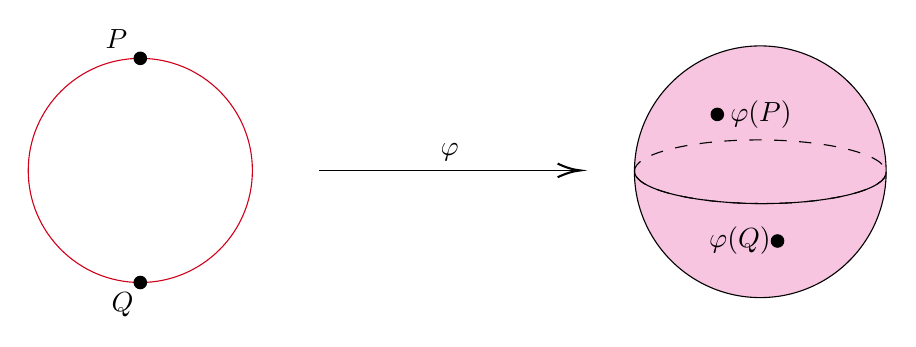
\begin{tikzpicture}[x=0.75pt,y=0.75pt,yscale=-1,xscale=1]
%uncomment if require: \path (0,300); %set diagram left start at 0, and has height of 300

%Shape: Circle [id:dp5720156977524582] 
\draw  [color={rgb, 255:red, 208; green, 2; blue, 27 }  ,draw opacity=1 ] (127,153) .. controls (127,123.18) and (151.18,99) .. (181,99) .. controls (210.82,99) and (235,123.18) .. (235,153) .. controls (235,182.82) and (210.82,207) .. (181,207) .. controls (151.18,207) and (127,182.82) .. (127,153) -- cycle ;
%Shape: Circle [id:dp1476626630307074] 
\draw  [fill={rgb, 255:red, 0; green, 0; blue, 0 }  ,fill opacity=1 ] (178,99) .. controls (178,97.34) and (179.34,96) .. (181,96) .. controls (182.66,96) and (184,97.34) .. (184,99) .. controls (184,100.66) and (182.66,102) .. (181,102) .. controls (179.34,102) and (178,100.66) .. (178,99) -- cycle ;
%Shape: Circle [id:dp6197701883715965] 
\draw  [fill={rgb, 255:red, 0; green, 0; blue, 0 }  ,fill opacity=1 ] (178,207) .. controls (178,205.34) and (179.34,204) .. (181,204) .. controls (182.66,204) and (184,205.34) .. (184,207) .. controls (184,208.66) and (182.66,210) .. (181,210) .. controls (179.34,210) and (178,208.66) .. (178,207) -- cycle ;
%Straight Lines [id:da7938139953077006] 
\draw    (267,153) -- (391,153) ;
\draw [shift={(393,153)}, rotate = 180] [color={rgb, 255:red, 0; green, 0; blue, 0 }  ][line width=0.75]    (10.93,-3.29) .. controls (6.95,-1.4) and (3.31,-0.3) .. (0,0) .. controls (3.31,0.3) and (6.95,1.4) .. (10.93,3.29)   ;
%Shape: Ellipse [id:dp903039161932605] 
\draw  [fill={rgb, 255:red, 247; green, 197; blue, 224 }  ,fill opacity=1 ] (419.07,153.64) .. controls (419.07,120.15) and (446.22,93) .. (479.71,93) .. controls (513.2,93) and (540.34,120.15) .. (540.34,153.64) .. controls (540.34,187.12) and (513.2,214.27) .. (479.71,214.27) .. controls (446.22,214.27) and (419.07,187.12) .. (419.07,153.64) -- cycle ;
%Shape: Arc [id:dp8603171310701756] 
\draw  [draw opacity=0] (540.34,153.64) .. controls (540.93,162.11) and (514.27,168.97) .. (480.78,168.97) .. controls (447.29,168.97) and (419.66,162.11) .. (419.07,153.64) -- (479.71,153.64) -- cycle ; \draw   (540.34,153.64) .. controls (540.93,162.11) and (514.27,168.97) .. (480.78,168.97) .. controls (447.29,168.97) and (419.66,162.11) .. (419.07,153.64) ;  
%Shape: Arc [id:dp40554050950174947] 
\draw  [draw opacity=0][dash pattern={on 4.5pt off 4.5pt}] (419.07,153.64) .. controls (419.07,153.64) and (419.07,153.64) .. (419.07,153.64) .. controls (418.48,145.16) and (445.15,138.3) .. (478.64,138.3) .. controls (512.12,138.3) and (539.75,145.16) .. (540.34,153.64) .. controls (540.93,162.11) and (514.27,168.97) .. (480.78,168.97) .. controls (447.29,168.97) and (419.66,162.11) .. (419.07,153.64) -- (479.71,153.64) -- cycle ; \draw  [dash pattern={on 4.5pt off 4.5pt}] (419.07,153.64) .. controls (419.07,153.64) and (419.07,153.64) .. (419.07,153.64) .. controls (418.48,145.16) and (445.15,138.3) .. (478.64,138.3) .. controls (512.12,138.3) and (539.75,145.16) .. (540.34,153.64) .. controls (540.93,162.11) and (514.27,168.97) .. (480.78,168.97) .. controls (447.29,168.97) and (419.66,162.11) .. (419.07,153.64) -- cycle ;  
%Shape: Circle [id:dp3795335580680428] 
\draw  [fill={rgb, 255:red, 0; green, 0; blue, 0 }  ,fill opacity=1 ] (456,126) .. controls (456,124.34) and (457.34,123) .. (459,123) .. controls (460.66,123) and (462,124.34) .. (462,126) .. controls (462,127.66) and (460.66,129) .. (459,129) .. controls (457.34,129) and (456,127.66) .. (456,126) -- cycle ;
%Shape: Circle [id:dp9731821727151901] 
\draw  [fill={rgb, 255:red, 0; green, 0; blue, 0 }  ,fill opacity=1 ] (485,187) .. controls (485,185.34) and (486.34,184) .. (488,184) .. controls (489.66,184) and (491,185.34) .. (491,187) .. controls (491,188.66) and (489.66,190) .. (488,190) .. controls (486.34,190) and (485,188.66) .. (485,187) -- cycle ;

% Text Node
\draw (176,95.6) node [anchor=south east] [inner sep=0.75pt]    {$P$};
% Text Node
\draw (179,210.4) node [anchor=north east] [inner sep=0.75pt]    {$Q$};
% Text Node
\draw (330,149.6) node [anchor=south] [inner sep=0.75pt]    {$\varphi $};
% Text Node
\draw (464,126) node [anchor=west] [inner sep=0.75pt]    {$\varphi ( P)$};
% Text Node
\draw (486,187) node [anchor=east] [inner sep=0.75pt]    {$\varphi ( Q)$};
\end{tikzpicture}
\caption{例4.7集合之示意图}
	\end{figure}
	\begin{figure}[h]
		\centering


\tikzset{every picture/.style={line width=0.75pt}} %set default line width to 0.75pt        

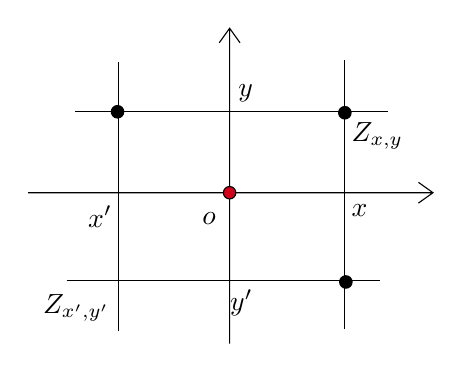
\begin{tikzpicture}[x=0.75pt,y=0.75pt,yscale=-1,xscale=1]
%uncomment if require: \path (0,300); %set diagram left start at 0, and has height of 300

%Shape: Axis 2D [id:dp12777471430843268] 
\draw  (123.46,160.92) -- (318.46,160.92)(220.49,81.67) -- (220.49,233.57) (311.46,155.92) -- (318.46,160.92) -- (311.46,165.92) (215.49,88.67) -- (220.49,81.67) -- (225.49,88.67)  ;
%Shape: Circle [id:dp5126442360837764] 
\draw  [fill={rgb, 255:red, 0; green, 0; blue, 0 }  ,fill opacity=1 ] (273,122.39) .. controls (273,120.73) and (274.34,119.39) .. (276,119.39) .. controls (277.66,119.39) and (279,120.73) .. (279,122.39) .. controls (279,124.05) and (277.66,125.39) .. (276,125.39) .. controls (274.34,125.39) and (273,124.05) .. (273,122.39) -- cycle ;
%Straight Lines [id:da9233924486508229] 
\draw    (167,98) -- (167,227.5) ;
%Shape: Circle [id:dp6689746044956462] 
\draw  [fill={rgb, 255:red, 208; green, 2; blue, 27 }  ,fill opacity=1 ] (217.49,160.92) .. controls (217.49,159.27) and (218.83,157.92) .. (220.49,157.92) .. controls (222.14,157.92) and (223.49,159.27) .. (223.49,160.92) .. controls (223.49,162.58) and (222.14,163.92) .. (220.49,163.92) .. controls (218.83,163.92) and (217.49,162.58) .. (217.49,160.92) -- cycle ;
%Straight Lines [id:da038234456342600476] 
\draw    (276,97) -- (276,226.5) ;
%Straight Lines [id:da02720895133232415] 
\draw    (146,122) -- (297,122) ;
%Straight Lines [id:da8732247039929291] 
\draw    (142,203) -- (293,203) ;
%Shape: Circle [id:dp9262510333566631] 
\draw  [fill={rgb, 255:red, 0; green, 0; blue, 0 }  ,fill opacity=1 ] (273.49,203.92) .. controls (273.49,202.27) and (274.83,200.92) .. (276.49,200.92) .. controls (278.14,200.92) and (279.49,202.27) .. (279.49,203.92) .. controls (279.49,205.58) and (278.14,206.92) .. (276.49,206.92) .. controls (274.83,206.92) and (273.49,205.58) .. (273.49,203.92) -- cycle ;
%Shape: Circle [id:dp8649857128324736] 
\draw  [fill={rgb, 255:red, 0; green, 0; blue, 0 }  ,fill opacity=1 ] (163.49,121.92) .. controls (163.49,120.27) and (164.83,118.92) .. (166.49,118.92) .. controls (168.14,118.92) and (169.49,120.27) .. (169.49,121.92) .. controls (169.49,123.58) and (168.14,124.92) .. (166.49,124.92) .. controls (164.83,124.92) and (163.49,123.58) .. (163.49,121.92) -- cycle ;

% Text Node
\draw (215.04,169.07) node [anchor=north east] [inner sep=0.75pt]    {$o$};
% Text Node
\draw (278,165.15) node [anchor=north west][inner sep=0.75pt]    {$x$};
% Text Node
\draw (223.5,118.6) node [anchor=south west] [inner sep=0.75pt]    {$y$};
% Text Node
\draw (219.5,206.4) node [anchor=north west][inner sep=0.75pt]    {$y'$};
% Text Node
\draw (165,166.15) node [anchor=north east] [inner sep=0.75pt]    {$x'$};
% Text Node
\draw (278,125.79) node [anchor=north west][inner sep=0.75pt]    {$Z_{x,y}$};
% Text Node
\draw (163.82,208.79) node [anchor=north east] [inner sep=0.75pt]    {$Z_{x',y'}$};


\end{tikzpicture}
\caption{例4.7证明$S^{2}\chadiao\dkh{\varphi(P),\varphi(Q)}$是连通的}
	\end{figure}
	
	
	
	
	设$Z_{x,y} = (\dkh{x}\times \mathbb{R})\cup(\dkh{y}\times \mathbb{R})$,由命题\ref{c4-m5}可知$Z_{x,y}$是连通的,而$\R^{2}\chadiao\dkh{(0,0)}\dabing_{x,y\neq 0}Z_{x,y}$,而这其中的集合族$\dkh{Z_{x,y}}_{x,y\in\R }$中任意两个集合之交$Z_{x,y}\cap Z_{x',y'} = \dkh{(x'.y),(x,y')}$非空。因此再由命题\ref{c4-m5}可知$R^{2}\chadiao\dkh{(0,0)}$是连通的。得证。
\end{proof}


\begin{proposition}[连通拓扑空间的乘积拓扑空间也是连通的]
	若$X,Y$为连通的拓扑空间,则$X\times Y$在乘积拓扑意义下也是连通的拓扑空间。
\end{proposition}
\begin{proof}
	记$Z_{x,y} =(\dkh{x}\times Y)\cup(\dkh{y}\times X)$那么由命题\ref{c4-m5}可知$Z_{x,y}$是连通的,而$X\times Y = \dabing_{(x,y)\in X\times Y}Z_{x,y}$,且$\dkh{(x,y')}\in Z_{x,y}\cap Z_{x',y'}\neq \emptyset$,因此再由命题\ref{c4-m5}可知$X\times Y$是连通的。
\end{proof}
\begin{example}[欧氏空间是连通的]
	$\R \times \R = \R^{2}$是连通的拓扑空间。
	\begin{note}
	以此类推$\R \times \R \times \cdots \R  = \R^{n}$也是连通的拓扑空间。	
	\end{note}
\end{example}
\begin{example}[欧氏空间中的单位球面是连通的]
	$B(0,1) = \dkh{x\in \mathbb{R}^{n}|||x||<1}$是连通的。
\end{example}
\begin{proof}
	只需证明:
	\begin{equation*}
		B(0,1)\cong \mathbb{R}^{n}
	\end{equation*}即可。事实上构造函数:
	\begin{equation*}
		\begin{aligned}
			B(0,1)&\longrightarrow \mathbb{R}^{n}\\
			x&\longmapsto \dfrac{x}{1-||x||}
		\end{aligned}
	\end{equation*}
	于是$y = \dfrac{x}{1-||x||}$,因此$||y|| = \dfrac{||x||}{1-||x||}$且$||x|| = \dfrac{||y||}{1+||y||}$,有$x = \dfrac{y}{1+||y||}$,都是连续的双射。
\end{proof}

\begin{proposition}[连通集合的闭包是连通的]\label{c4-m7}
	设$X$为一个拓扑空间,$Y\subset X$是连通的,则$\overline{Y}$是连通的。
\end{proposition}
\begin{proof}
	设$\overline{Y} = U\sqcup V;\tl{\emptyset\neq  U,V\subset_{open,closed}\overline{Y}}$,因此$Y = (Y\cap U)\sqcup (Y\cap V)$,由于\lanse{$Y$是连通的},因此$Y\cap U  =Y$或者$Y\cap V=Y$,不妨设$Y\cap U=Y$则$Y\subset U$,又因为$U$是闭集,因此\tl{$\overline{Y}\subset U$},因此$U =\overline{Y}$,则$V = \emptyset$矛盾!
\end{proof}


\begin{example}[二维单位球面是连通的]
	$S^{2}$是在欧氏拓扑意义下是连通的。
\end{example}
\begin{proof}
	仍然给出两个证明:
	\begin{enumerate}
		\item 我们已经知道$S^{2}\chadiao \dkh{P}\cong \mathbb{R}^{2}$是连通的。而若取$P\neq P'$就有$S^{2}=(S^{2}\chadiao \dkh{P})\cup(S^{2}\chadiao \dkh{P'})$是连通的。
		\item 直接由命题\ref{c4-m7}可得,由于$S^{2}\chadiao \dkh{P}\cong \mathbb{R}^{2}$是连通的,则$\overline{S^{2}\chadiao\dkh{P}}$是连通的、
	\end{enumerate}
\end{proof}

\subsection{连通分支}
根据我们上面的讨论可以知道,连通性其实一个比较难达到的性质,但是有些不连通的拓扑空间的某些部分是连通的,因此我们引入下面的连通分支的概念:
\begin{definition}[连通分支]
	设$X$为一个拓扑空间,如果子集$Y\subset X$满足:
	\begin{enumerate}
	\item $Y$是连通的。(\tl{确保连通分支是连通的})
	\item $\forall Y'\subset X$是连通的,且$Y'\supset Y$,则$Y=  Y'$。(\tl{意思就是连通分支在连通分支中的极大性})	
	\end{enumerate}
	就称$Y$为$X$的一个\gn{连通分支}。
\end{definition}
\begin{proposition}[连通分支的存在性]
	设$X$为一个拓扑空间,则$X$可以表示为若干连通分支的无交并。
\end{proposition}
\begin{proof}
固定$x_{0}\in X$,记$S_{x_{0}} = \dkh{F\subset X|F\text{连通},x_{0}\in F}$,令$X_{x_{0}} = \dabing_{F\in S}F $,那么$X_{x_{0}}$连通。

$\forall Y\subset X$为包含$X_{x_{0}}$的连通集,$Y\supset X_{x_{0}}\ni $,则$Y\in S_{x_{0}}$,则$Y = X_{x_{0}}$,那么$X_{x_{0}}$为$X$中的一个连通分支。

观察到连通分支$X_{x_{1}}$与$X_{x_{2}}$之间有这样两类的关系:
\begin{enumerate}
	\item $X_{x_{1}}\cap X_{x_{2}} = \emptyset$
	\item $X_{x_{1}}\cap X_{x_{2}} \neq  \emptyset$,那么$X_{x_{1}} = X_{x_{2}}$
\end{enumerate}

那么提出重复的连通分支后,设$\dkh{X_{x_{i}}|i\in I}$为互不相交的连通分支,则:
	\begin{equation}\label{c4-eq1}
		X = \bigsqcup_{i\in I}X_{x_{i}}
	\end{equation}
\end{proof}
\begin{proposition}[连通分支为闭集]\label{c4-m9}
	连通分支必为闭集
\end{proposition}
\begin{proof}
	设$F\subset X$为连通分支。$\overline{F}$是连通的,因此$\overline{F}\supset F$,则$\overline{F} = F$,说明$F$是闭集。
\end{proof}

\begin{note}
在分解式\ref{c4-eq1}中,$\dkh{X_{x_{i}} |i\in I}$已经是$X$的全部连通分支(\tl{意思就是这些分解已经囊括了所有的$X$的连通分支})。	
\begin{proof}
	任取$Y\subset X$为$X$的连通分支,那么$Y$就可以写作:
	\begin{equation*}
		Y = \bigsqcup_{i\in I}(Y\cap X_{x_{i}})
	\end{equation*}
	
	其中$Y\cap X_{x_{i}}$是$Y$中闭集(由命题\ref{c4-m9}),设$y_{0}\in Y\subset X$,则$\exists i_{0},\st y_{0}\in X_{i_{0}}$,那么$Y,X_{i_{0}}$为包含$y_{0}$的连通分支。则$Y\cup X_{i_{0}}$是连通的。
\end{proof}
\end{note}
\begin{corollary}[连通分支放在一起就构成了整个集合]
	设$\dkh{X_{i}|i\in I}$为$X$的全部连通分支,则:
	\begin{equation*}
		X = \bigsqcup_{i\in I}X_{i}
	\end{equation*}
\end{corollary}

\begin{note}
(\tl{连通分支中的非空连通闭集就是连通分支})若$\exists X$的有限个非空的连通闭集$F_{i},i=1,2,\cdots , n$,则$F_{i}$必等于某连通分支,即:$X = \bigsqcup_{i = 1}^{n}F_{i}$中的$\dkh{F_{i}|i=1,2,\cdots ,n}$为$X$的全部连通分支。

\begin{proof}
	设$\dkh{X_{i}|i\in I}$为$X$的连通分支集,即满足:\begin{equation*}
		X = \bigsqcup_{i\in I}X_{i}
	\end{equation*}
	根据条件,我们还有:
	\begin{equation*}
		X = \bigsqcup_{i=1}^{n}F_{i}
	\end{equation*}
	那么就有$X_{i} = \bigsqcup_{j=1}^{n}(F_{j}\cap X_{i})$,则$\exists j_{0},
	\st X_{i}=F_{j_{0}}\cap X_{i}$,那么$X_{i}\subset F_{j_{0}}$因此$X_{i} = F_{j_{0}}$。
	
	也就是说这边是给定一个$i$就会出来一个$j,\st X_{i} = F_{j}$那么就有:
	\begin{equation*}
		\dkh{X_{i}|i\in I}\subset \dkh{F_{i}|i=1,2,\cdots ,n}
	\end{equation*}假设$\exists F_{i}\neq X_{j} ,\forall j\in X$,就有:
	\begin{equation*}
		X = \bigsqcup_{j\in I}X_{j} = \bigsqcup_{k}F_{i_{k}}
	\end{equation*}
	因此$F_{i}\cap(\bigsqcup_{k}F_{i_{k}}) = \emptyset$,那么$F_{i} = \emptyset$,与$F_{i}$非空矛盾!
	
	因此$\dkh{F_{i}|i=1,2,\cdots,n}$就是$X$的全部连通分支。
\end{proof}	
\end{note}
\begin{example}[不连通集$\mathbb{Q}$的连通分支]
	有理数集$\mathbb{Q}\subset\mathbb{R}$满足:
	\begin{equation*}
		\mathbb{Q} = \bigsqcup_{q\in \mathbb{Q}}\dkh{q}
	\end{equation*}
	\begin{proof}
		只要证$\forall X\subset \mathbb{Q},\dkh{q}\sqsubset X$,则$X$不连通即可。不然,则$\exists q'\in X(q\neq q')$,由于实数的稠密性可知,$\exists x\in \mathbb{R}\chadiao\mathbb{Q}$,那么$X = ((-\infty ,x)\cap X)\sqcup((x,+\infty)\cap X)$。
		
		\begin{figure}[h]
			\centering
			

\tikzset{every picture/.style={line width=0.75pt}} %set default line width to 0.75pt        

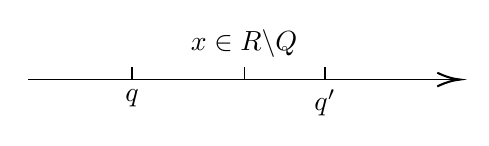
\begin{tikzpicture}[x=0.75pt,y=0.75pt,yscale=-1,xscale=1]
%uncomment if require: \path (0,300); %set diagram left start at 0, and has height of 300

%Straight Lines [id:da04645423172406837] 
\draw    (120,132) -- (326,132) ;
\draw [shift={(328,132)}, rotate = 180] [color={rgb, 255:red, 0; green, 0; blue, 0 }  ][line width=0.75]    (10.93,-3.29) .. controls (6.95,-1.4) and (3.31,-0.3) .. (0,0) .. controls (3.31,0.3) and (6.95,1.4) .. (10.93,3.29)   ;
%Straight Lines [id:da5717959472622021] 
\draw    (224,126) -- (224,132) ;
%Straight Lines [id:da5565885417046166] 
\draw    (170,126) -- (170,132) ;
%Straight Lines [id:da25972787960227084] 
\draw    (263,126) -- (263,132) ;

% Text Node
\draw (170,135.4) node [anchor=north] [inner sep=0.75pt]    {$q$};
% Text Node
\draw (263,135.4) node [anchor=north] [inner sep=0.75pt]    {$q'$};
% Text Node
\draw (224,122.6) node [anchor=south] [inner sep=0.75pt]    {$x\in \mathbb{R}\chadiao\mathbb{Q}$};


\end{tikzpicture}
\caption{例4.11之区间关系}
		\end{figure}
		
		这俩集合都是非空的(因为$q\in ((-\infty ,x)\cap X),q'\in ((x,+\infty)\cap X)$)。因此$X$不连通,
	\end{proof}
\end{example}
\section{道路连通性}
\begin{definition}[道路]
	设$X$为拓扑空间,$X$中的一个连续映射$\gamma :[0,1]\longrightarrow X$称为$X$中的一条\gn{道路}。
\end{definition}
\subsection{道路连通性与例}
\begin{definition}[道路连通]
	设$X$为拓扑空间,如果对于$\forall p,q\in X,\exists$道路$\gamma :[0,1]\longrightarrow X,\st \gamma(0)=p,\gamma(1)=q$,就称$X$是\gn{道路连通的}。
\end{definition}
\begin{example}[$\R$中区间是道路连通的]
	设$I\subset \R $为区间,则$\forall p,q\in I,\gamma(t) = tp+(1-t)q$是一条道路。
\end{example}
\subsection{道路连通性为拓扑不变性}
\begin{proposition}[道路连通性是一个拓扑不变性]\label{c4-m10}
	设$X,Y$为拓扑空间,设$f:X\longrightarrow Y$是连续映射,$X$是道路连通的,则$f(X)$也是道路连通的。
\end{proposition}
\begin{proof}映射之关系如图所示:
	
	\begin{figure}[h]
		\centering
		

\tikzset{every picture/.style={line width=0.75pt}} %set default line width to 0.75pt        

\begin{tikzpicture}[x=0.75pt,y=0.75pt,yscale=-1,xscale=1]
%uncomment if require: \path (0,300); %set diagram left start at 0, and has height of 300

%Curve Lines [id:da16539869633767168] 
\draw    (249,135) .. controls (289,105) and (317,124.5) .. (329,128.5) .. controls (341,132.5) and (355,140.5) .. (346,194.5) .. controls (337,248.5) and (224,160) .. (249,135) -- cycle ;
%Curve Lines [id:da4419452394973107] 
\draw    (450,149) .. controls (438,119.5) and (534,103.5) .. (530,142.5) .. controls (526,181.5) and (578,182.5) .. (547,208.5) .. controls (516,234.5) and (472,205.5) .. (450,149) -- cycle ;
%Curve Lines [id:da7140903966701106] 
\draw [color={rgb, 255:red, 208; green, 2; blue, 27 }  ,draw opacity=1 ]   (271,142.5) .. controls (298.79,144.21) and (299.01,165.4) .. (311.05,184.07) ;
\draw [shift={(312,185.5)}, rotate = 235.62] [color={rgb, 255:red, 208; green, 2; blue, 27 }  ,draw opacity=1 ][line width=0.75]    (10.93,-3.29) .. controls (6.95,-1.4) and (3.31,-0.3) .. (0,0) .. controls (3.31,0.3) and (6.95,1.4) .. (10.93,3.29)   ;
%Curve Lines [id:da058857475357372735] 
\draw [color={rgb, 255:red, 208; green, 2; blue, 27 }  ,draw opacity=1 ]   (475,145.5) .. controls (483,164.5) and (502.25,163.88) .. (508.63,169.69) .. controls (514.81,175.33) and (513.11,182.08) .. (529.43,192.52) ;
\draw [shift={(531,193.5)}, rotate = 211.43] [color={rgb, 255:red, 208; green, 2; blue, 27 }  ,draw opacity=1 ][line width=0.75]    (10.93,-3.29) .. controls (6.95,-1.4) and (3.31,-0.3) .. (0,0) .. controls (3.31,0.3) and (6.95,1.4) .. (10.93,3.29)   ;
%Straight Lines [id:da6748570416163333] 
\draw    (158,168) -- (239,168) ;
\draw [shift={(241,168)}, rotate = 180] [color={rgb, 255:red, 0; green, 0; blue, 0 }  ][line width=0.75]    (10.93,-3.29) .. controls (6.95,-1.4) and (3.31,-0.3) .. (0,0) .. controls (3.31,0.3) and (6.95,1.4) .. (10.93,3.29)   ;
%Straight Lines [id:da630763668736043] 
\draw    (365,168) -- (445,168) ;
\draw [shift={(447,168)}, rotate = 180] [color={rgb, 255:red, 0; green, 0; blue, 0 }  ][line width=0.75]    (10.93,-3.29) .. controls (6.95,-1.4) and (3.31,-0.3) .. (0,0) .. controls (3.31,0.3) and (6.95,1.4) .. (10.93,3.29)   ;

% Text Node
\draw (156,168) node [anchor=east] [inner sep=0.75pt]    {$[ 0,1]$};
% Text Node
\draw (322,137.4) node [anchor=north west][inner sep=0.75pt]    {$X$};
% Text Node
\draw (493,128.4) node [anchor=north west][inner sep=0.75pt]    {$f( X)$};
% Text Node
\draw (199.5,164.6) node [anchor=south] [inner sep=0.75pt]    {$\gamma $};
% Text Node
\draw (406,164.6) node [anchor=south] [inner sep=0.75pt]    {$f$};
% Text Node
\draw (273,139.1) node [anchor=south west] [inner sep=0.75pt]    {$p'$};
% Text Node
\draw (314,188.9) node [anchor=north west][inner sep=0.75pt]    {$q'$};
% Text Node
\draw (473,145.5) node [anchor=east] [inner sep=0.75pt]    {$p$};
% Text Node
\draw (529,196.9) node [anchor=north east] [inner sep=0.75pt]    {$q$};
% Text Node
\draw (283,164.2) node [anchor=west] [inner sep=0.75pt]    {$\gamma $};
% Text Node
\draw (475,176.2) node [anchor=west] [inner sep=0.75pt]    {$f\circ \gamma $};


\end{tikzpicture}\caption{命题\ref{c4-m10}之映射关系图}
	\end{figure}
		设道路为:
	\begin{equation*}
		\begin{aligned}
			\gamma [0,1]&\longrightarrow X\\
			t&\longmapsto \gamma(t)
		\end{aligned}
	\end{equation*}
	
	由于$X$是道路连通的,因此选择一条道路$p'q'\in X$,由于$f$是连续映射,那么$f\circ \gamma$是$f(X)$中起点为$p = f\circ \gamma(p')$,终点为$q = f\circ \gamma(q')$的道路。因此$f(X)$是道路连通的。
\end{proof}
\begin{corollary}
	若$X\cong Y$,则$X$道路连通$\iff Y$道路连通。
\end{corollary}

和紧性一样,定义了道路连通,首先的问题是道路连通与连通性是什么关系呢?
\begin{proposition}[道路连通性蕴含连通性]\label{c4-m11}
	设$X$是道路连通的,则$X$是连通的。
\end{proposition}
\begin{proof}
	若$X = U\sqcup V$,其中$U,V\subset_{open},U\neq \emptyset ,V\neq \emptyset$,取$\forall P\in U,Q\in V$,假设$\gamma :[0,1]\longrightarrow X$为道路。
	
	\begin{figure}[h]
		\centering


\tikzset{every picture/.style={line width=0.75pt}} %set default line width to 0.75pt        

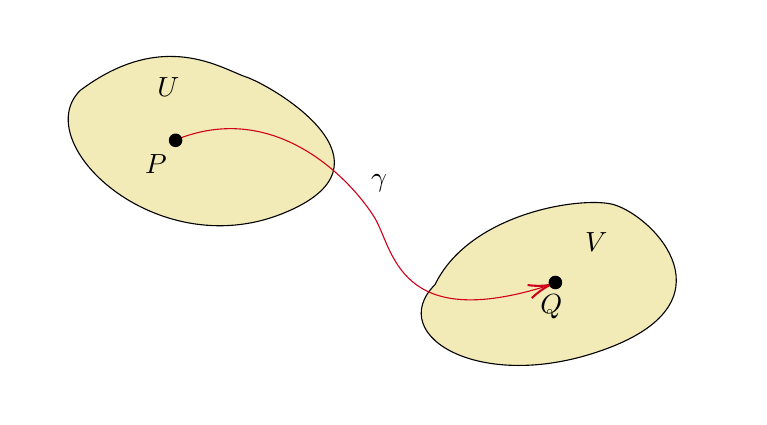
\begin{tikzpicture}[x=0.75pt,y=0.75pt,yscale=-1,xscale=1]
%uncomment if require: \path (0,300); %set diagram left start at 0, and has height of 300

%Curve Lines [id:da7863194874225077] 
\draw [fill={rgb, 255:red, 243; green, 235; blue, 183 }  ,fill opacity=1 ]   (165,66) .. controls (205,36) and (233,55.5) .. (245,59.5) .. controls (257,63.5) and (323,101.5) .. (262,125.5) .. controls (201,149.5) and (140,91) .. (165,66) -- cycle ;
%Curve Lines [id:da5888643693255495] 
\draw [fill={rgb, 255:red, 243; green, 235; blue, 183 }  ,fill opacity=1 ]   (336,159.5) .. controls (352,126.5) and (402,117.5) .. (420,120.5) .. controls (438,123.5) and (482,165.5) .. (421,189.5) .. controls (360,213.5) and (311,184.5) .. (336,159.5) -- cycle ;
%Curve Lines [id:da5690842124217828] 
\draw [color={rgb, 255:red, 208; green, 2; blue, 27 }  ,draw opacity=1 ]   (213,89) .. controls (262,70.5) and (298,112.5) .. (307,127.5) .. controls (315.96,142.43) and (317.98,183.09) .. (390.9,159.86) ;
\draw [shift={(392,159.5)}, rotate = 162.03] [color={rgb, 255:red, 208; green, 2; blue, 27 }  ,draw opacity=1 ][line width=0.75]    (10.93,-3.29) .. controls (6.95,-1.4) and (3.31,-0.3) .. (0,0) .. controls (3.31,0.3) and (6.95,1.4) .. (10.93,3.29)   ;
%Shape: Circle [id:dp17641741974455116] 
\draw  [fill={rgb, 255:red, 0; green, 0; blue, 0 }  ,fill opacity=1 ] (208,90) .. controls (208,88.34) and (209.34,87) .. (211,87) .. controls (212.66,87) and (214,88.34) .. (214,90) .. controls (214,91.66) and (212.66,93) .. (211,93) .. controls (209.34,93) and (208,91.66) .. (208,90) -- cycle ;
%Shape: Circle [id:dp21123219693785167] 
\draw  [fill={rgb, 255:red, 0; green, 0; blue, 0 }  ,fill opacity=1 ] (391,158.5) .. controls (391,156.84) and (392.34,155.5) .. (394,155.5) .. controls (395.66,155.5) and (397,156.84) .. (397,158.5) .. controls (397,160.16) and (395.66,161.5) .. (394,161.5) .. controls (392.34,161.5) and (391,160.16) .. (391,158.5) -- cycle ;

% Text Node
\draw (201,58.4) node [anchor=north west][inner sep=0.75pt]    {$U$};
% Text Node
\draw (208,95.4) node [anchor=north east] [inner sep=0.75pt]    {$P$};
% Text Node
\draw (407,133.4) node [anchor=north west][inner sep=0.75pt]    {$V$};
% Text Node
\draw (392,162.9) node [anchor=north] [inner sep=0.75pt]    {$Q$};
% Text Node
\draw (304,116) node [anchor=south west] [inner sep=0.75pt]    {$\gamma $};


\end{tikzpicture}\caption{命题\ref{c4-m11}之集合}
	\end{figure}
	
	那么:$\gamma(0)=P,\gamma(1)=Q$,则连通集合$[0,1]=\gamma^{-1}(U)\sqcup \gamma^{-1}(V)$,其中$P\in \gamma^{-1}(U),Q\in \gamma^{-1}(V)$,均非空,因此矛盾。
\end{proof}
\begin{example}[连通但不道路连通的例子---拓扑学家的正弦曲线]\label{c4-l13}
	设拓扑空间$X \subset \R^{2} $赋予子空间拓扑,且$X :=Y\sqcup Z$,其中:
	\begin{figure}[h]
		\centering
		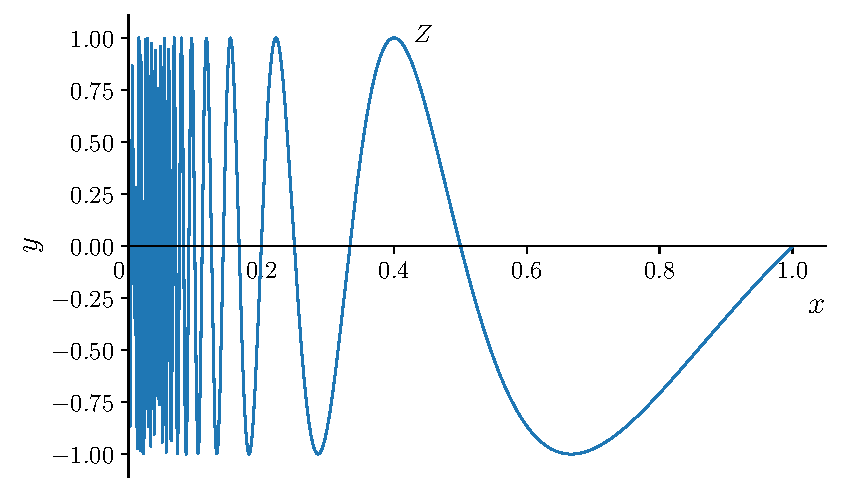
\includegraphics[scale=0.6]{图片/sin_1.pdf}
		\caption{例\ref{c4-l13}之函数图像}
	\end{figure}
	\begin{equation*}
		Y=\dkh{(x,y)|-1\leq y \leq 1}
	\end{equation*}
	\begin{equation*}
		Z = \dkh{(x,\sin\dfrac{\pi}{x})|0<x\leq 1}
	\end{equation*}
	我们断言下两点:
	\begin{itemize}
		\item 首先我们说明\lei{$X$是连通的},这是因为很明显有$X = \overline{Z}$,并且$Z$是连通的(从函数的构造可以知道)。
		\item 其次\lei{$X$不是道路连通的}。
	\end{itemize}
\end{example}
\begin{proof}
	反设$\exists\gamma:[0,1]\longrightarrow X,\st \gamma(0)\in Y,\gamma(1)\in Z$,因为$Y$是闭集,因此$\gamma^{-1}(Y)\subset_{closed}[0,1]$,下只需证明$\gamma^{-1}(Y)$是开集。
	
	这只需要证$\forall t_{0}\in \gamma^{-1}(Y),\exists \delta>0,\st (t_{0}-\delta,t_{0}+\delta)\cap[0,1]\subset \gamma^{-1}(Y)$。
	
	对于$\gamma(t_{0})\in Y$,取一个足够小的$\gamma(t_{0})$的开的矩形邻域$U$,那么$U\cap X$如下所示:
	\begin{figure}[h]
		\centering
		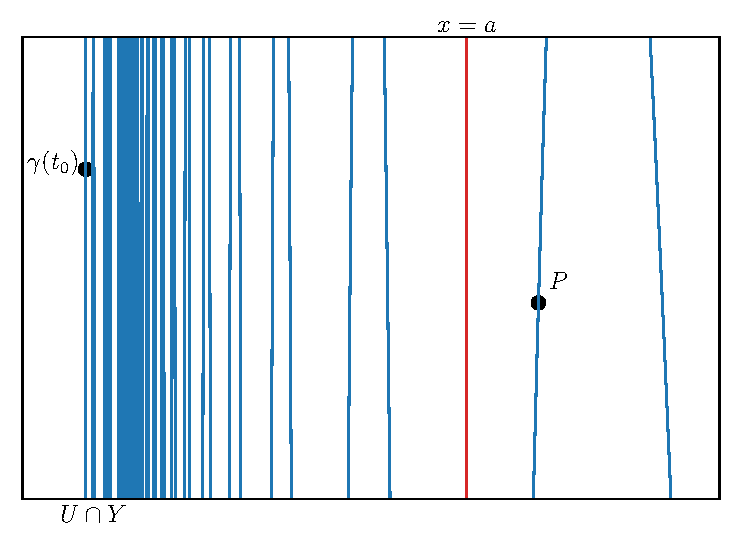
\includegraphics[scale=0.6]{图片/sin_2.pdf}
		\caption{例\ref{c4-l13}之$U\cap X$}
	\end{figure}
	
	下断言:\lei{$U\cap Y$为$U\cap X$的一个连通分支。}
	
	$\blacktriangleright$这是因为:$\forall U\cap Y\sqsubset F\subset U\cap X$,取$p\in F$,且$p\in U\cap Z$,根据实数的稠密性,必然$\exists a$使得$F = (\dkh{x\leq a}\cap F)\sqcup (\dkh{x\geq a}\cap F)$。$\blacktriangleleft$
	
	设$\gamma^{-1}(U)$为包含$t_{0}$的一个开邻域,则$\exists \delta>0,\st I=(t_{0}-\delta,t_{0}+\delta)\cap [0,1]\subset \gamma^{-1}(U)$,那么:
	\begin{enumerate}
		\item $\gamma(I)$连通
		\item $\gamma(I)\ni \gamma{t_{0}} $则$\gamma(I)\cap(U\cap Y)\neq \emptyset$
		\item $U\cap Y$为$U\cap X$的一个连通分支。
	\end{enumerate}
	
	因此$\gamma(I)\subset U\cap Y$,因此$I\subset \gamma^{-1}(Y)$。
	
\end{proof}
\begin{note}
道路连通的连通分支的闭包不必为闭集。	
\end{note}
\begin{definition}[局部道路连通]
	设$X$为拓扑空间,若$\forall p\in X.\forall p$的开邻域$U$,总存在$p$的道路连通的且含于$U$的开邻域$V$,则称$X$是\gn{局部道路连通}的。
\end{definition}

\begin{note}
若$X$是局部道路连通的,则:
\begin{equation}\label{c4-eq2}
	\forall p\in X,\exists p\text{的道路连通的开邻域。}	
\end{equation}
\end{note}
\begin{proof}
	这是上定义的直接缩小。
\end{proof}



\begin{lemma}[Glueing引理]\label{c4-y1}
	设$X = Y\cup Z,f:Y\longrightarrow W,g:Z\longrightarrow W$均为连续映射,$f|_{Y\cap Z} = g|_{Y\cap Z}$,设$Y,Z$均为闭集,定义:
	\begin{equation*}
		\begin{aligned}
			f\cup g:X&\longrightarrow W\\
			p&\longmapsto \hanshu{&f(p),p\in Y\\
			&g(p),p\in Z}
		\end{aligned}
	\end{equation*}
	则$f\cup g$是连续映射。
\end{lemma}	
\begin{proof}
	$\forall F\subset_{closed}W,(f\cup g)^(-1)(F) = f^{-1}(F)\cup g^{-1}(F)\subset_{closed}X$,最后一步是因为$f,g$均为连续映射,那么$f^{-1}(F)$为$Y$中闭集,$g^{-1}(F)$为$Z$中闭集,因此他俩均为$X$中闭集。
\end{proof}
\begin{proposition}\label{c4-m12}
	局部道路连通的连通拓扑空间是道路连通的拓扑空间。
\end{proposition}
\begin{note}
实际上连通拓扑空间满足性质\ref{c4-eq2},就是道路连通的了(从证明可以看出来)。	
\end{note}
\begin{proof}
设$X$是连通的,并且局部道路连通,要证$X$是道路连通的,取$p_{0}\in X,S=\dkh{p\in X|\exists\text{道路}\gamma,\st \gamma(0) = p_{0},\gamma(1) = p}$。下只需证$S =X$即可。

$\blacktriangleright$这是因为,我们可以这样看待集合$S$,集合$X$中的连通道路都可以通过此两种操作通过$S$进行构造:
\begin{figure}[h]
	\centering
	

\tikzset{every picture/.style={line width=0.75pt}} %set default line width to 0.75pt        

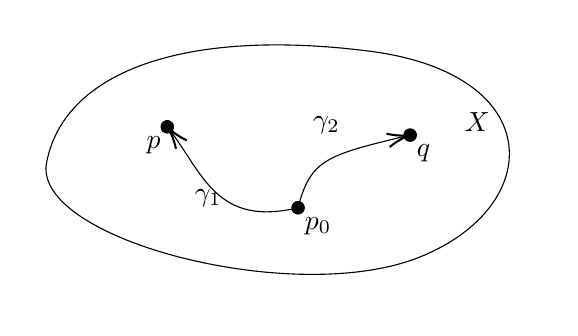
\begin{tikzpicture}[x=0.75pt,y=0.75pt,yscale=-1,xscale=1]
%uncomment if require: \path (0,300); %set diagram left start at 0, and has height of 300

%Curve Lines [id:da849424854437286] 
\draw    (152,95) .. controls (161,51) and (220,31) .. (307,42) .. controls (394,53) and (392,117.5) .. (331,141.5) .. controls (270,165.5) and (143,132) .. (152,95) -- cycle ;
%Shape: Circle [id:dp6204923445616997] 
\draw  [fill={rgb, 255:red, 0; green, 0; blue, 0 }  ,fill opacity=1 ] (207,78.5) .. controls (207,76.84) and (208.34,75.5) .. (210,75.5) .. controls (211.66,75.5) and (213,76.84) .. (213,78.5) .. controls (213,80.16) and (211.66,81.5) .. (210,81.5) .. controls (208.34,81.5) and (207,80.16) .. (207,78.5) -- cycle ;
%Shape: Circle [id:dp26857039968349916] 
\draw  [fill={rgb, 255:red, 0; green, 0; blue, 0 }  ,fill opacity=1 ] (270,117.5) .. controls (270,115.84) and (271.34,114.5) .. (273,114.5) .. controls (274.66,114.5) and (276,115.84) .. (276,117.5) .. controls (276,119.16) and (274.66,120.5) .. (273,120.5) .. controls (271.34,120.5) and (270,119.16) .. (270,117.5) -- cycle ;
%Shape: Circle [id:dp23654368410237447] 
\draw  [fill={rgb, 255:red, 0; green, 0; blue, 0 }  ,fill opacity=1 ] (324,82.5) .. controls (324,80.84) and (325.34,79.5) .. (327,79.5) .. controls (328.66,79.5) and (330,80.84) .. (330,82.5) .. controls (330,84.16) and (328.66,85.5) .. (327,85.5) .. controls (325.34,85.5) and (324,84.16) .. (324,82.5) -- cycle ;
%Curve Lines [id:da33957480200046386] 
\draw    (211.26,80.12) .. controls (227.32,101.33) and (234,126.76) .. (273,117.5) ;
\draw [shift={(210,78.5)}, rotate = 51.67] [color={rgb, 255:red, 0; green, 0; blue, 0 }  ][line width=0.75]    (10.93,-3.29) .. controls (6.95,-1.4) and (3.31,-0.3) .. (0,0) .. controls (3.31,0.3) and (6.95,1.4) .. (10.93,3.29)   ;
%Curve Lines [id:da8390265271686743] 
\draw    (273,117.5) .. controls (278.91,94.35) and (286.76,92.06) .. (325.22,82.92) ;
\draw [shift={(327,82.5)}, rotate = 166.64] [color={rgb, 255:red, 0; green, 0; blue, 0 }  ][line width=0.75]    (10.93,-3.29) .. controls (6.95,-1.4) and (3.31,-0.3) .. (0,0) .. controls (3.31,0.3) and (6.95,1.4) .. (10.93,3.29)   ;

% Text Node
\draw (275,120.9) node [anchor=north west][inner sep=0.75pt]    {$p_{0}$};
% Text Node
\draw (208,81.9) node [anchor=north east] [inner sep=0.75pt]    {$p$};
% Text Node
\draw (329,85.9) node [anchor=north west][inner sep=0.75pt]    {$q$};
% Text Node
\draw (229.7,107.4) node [anchor=north] [inner sep=0.75pt]    {$\gamma _{1}$};
% Text Node
\draw (286.7,72.4) node [anchor=north] [inner sep=0.75pt]    {$\gamma _{2}$};
% Text Node
\draw (352,70.4) node [anchor=north west][inner sep=0.75pt]    {$X$};


\end{tikzpicture}
\caption{命题\ref{c4-m12}“只要证”之说明}
\end{figure}
\begin{enumerate}
	\item \lanse{道路反过来走}:$\gamma:[0,1]\longrightarrow X$,定义:
	\begin{equation*}
		\begin{aligned}
			\gamma^{-1}:[0,1]&\longrightarrow X\\
			t&\longmapsto \gamma(1-t)
		\end{aligned}
	\end{equation*}
	\item \lanse{道路接起来}:设$\gamma_{1},\gamma_{2}:[0,1]\longrightarrow X$为道路,$\gamma_{1} = \gamma_{2}(0)$,定义:
	\begin{equation*}
		\begin{aligned}
			\gamma = \gamma_{1}\circ\gamma_{2} [0,1]
		&\longrightarrow X\\
		t&\longmapsto \hanshu{&\gamma_{1}(2t),0\leq t\leq\dfrac{1}{2}\\
		&\gamma_{2}(2t-1),\dfrac{1}{2}\leq t\leq 1}
		\end{aligned}
	\end{equation*}
\end{enumerate}而这又由于引理\ref{c4-y1}可知,这样的映射$\gamma$是连续的。$\blacktriangleleft$





由于$S$是连通的,则只需要证$S$既开又闭即可。

\begin{enumerate}
	\item \lanse{若$S$是开集},则$\forall p\in S,\exists p$的开邻域$U,\st U\subset S$。
	\begin{figure}[h]
		\centering

\tikzset{every picture/.style={line width=0.75pt}} %set default line width to 0.75pt        

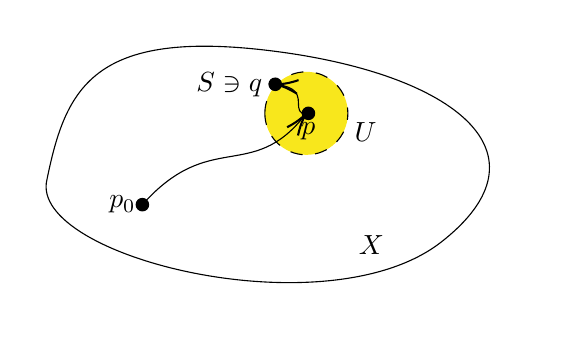
\begin{tikzpicture}[x=0.75pt,y=0.75pt,yscale=-1,xscale=1]
%uncomment if require: \path (0,300); %set diagram left start at 0, and has height of 300

%Curve Lines [id:da5717965138672669] 
\draw    (172,164) .. controls (181,120) and (194,91) .. (281,102) .. controls (368,113) and (417,151) .. (362,194) .. controls (307,237) and (163,201) .. (172,164) -- cycle ;
%Shape: Circle [id:dp46404817304840984] 
\draw  [fill={rgb, 255:red, 248; green, 231; blue, 28 }  ,fill opacity=1 ][dash pattern={on 4.5pt off 4.5pt}] (277,132) .. controls (277,120.95) and (285.95,112) .. (297,112) .. controls (308.05,112) and (317,120.95) .. (317,132) .. controls (317,143.05) and (308.05,152) .. (297,152) .. controls (285.95,152) and (277,143.05) .. (277,132) -- cycle ;
%Curve Lines [id:da9713828285003865] 
\draw    (218,176) .. controls (250.51,139.55) and (270.4,165.2) .. (295.83,133.49) ;
\draw [shift={(297,132)}, rotate = 127.41] [color={rgb, 255:red, 0; green, 0; blue, 0 }  ][line width=0.75]    (10.93,-3.29) .. controls (6.95,-1.4) and (3.31,-0.3) .. (0,0) .. controls (3.31,0.3) and (6.95,1.4) .. (10.93,3.29)   ;
%Shape: Circle [id:dp31815568627463153] 
\draw  [fill={rgb, 255:red, 0; green, 0; blue, 0 }  ,fill opacity=1 ] (295,132) .. controls (295,130.34) and (296.34,129) .. (298,129) .. controls (299.66,129) and (301,130.34) .. (301,132) .. controls (301,133.66) and (299.66,135) .. (298,135) .. controls (296.34,135) and (295,133.66) .. (295,132) -- cycle ;
%Shape: Circle [id:dp14359583316159896] 
\draw  [fill={rgb, 255:red, 0; green, 0; blue, 0 }  ,fill opacity=1 ] (215,176) .. controls (215,174.34) and (216.34,173) .. (218,173) .. controls (219.66,173) and (221,174.34) .. (221,176) .. controls (221,177.66) and (219.66,179) .. (218,179) .. controls (216.34,179) and (215,177.66) .. (215,176) -- cycle ;
%Curve Lines [id:da032394262122533934] 
\draw    (284.14,118.31) .. controls (298.22,120.8) and (290.23,129.14) .. (295,132) ;
\draw [shift={(282,118)}, rotate = 6.71] [color={rgb, 255:red, 0; green, 0; blue, 0 }  ][line width=0.75]    (10.93,-3.29) .. controls (6.95,-1.4) and (3.31,-0.3) .. (0,0) .. controls (3.31,0.3) and (6.95,1.4) .. (10.93,3.29)   ;
%Shape: Circle [id:dp02758863898796493] 
\draw  [fill={rgb, 255:red, 0; green, 0; blue, 0 }  ,fill opacity=1 ] (279,118) .. controls (279,116.34) and (280.34,115) .. (282,115) .. controls (283.66,115) and (285,116.34) .. (285,118) .. controls (285,119.66) and (283.66,121) .. (282,121) .. controls (280.34,121) and (279,119.66) .. (279,118) -- cycle ;

% Text Node
\draw (321,189.4) node [anchor=north west][inner sep=0.75pt]    {$X$};
% Text Node
\draw (216,176) node [anchor=east] [inner sep=0.75pt]    {$p_{0}$};
% Text Node
\draw (277,118) node [anchor=east] [inner sep=0.75pt]    {$S\ni q$};
% Text Node
\draw (319,135.4) node [anchor=north west][inner sep=0.75pt]    {$U$};
% Text Node
\draw (298,135.4) node [anchor=north] [inner sep=0.75pt]    {$p$};


\end{tikzpicture}\caption{命题\ref{c4-m12}中之$S$为开集}
	\end{figure}
	\item \lanse{若$S$是闭集},则$\forall S$的极限点$p$,$p\in S$。
	\begin{figure}[h]
		\centering
		

\tikzset{every picture/.style={line width=0.75pt}} %set default line width to 0.75pt        

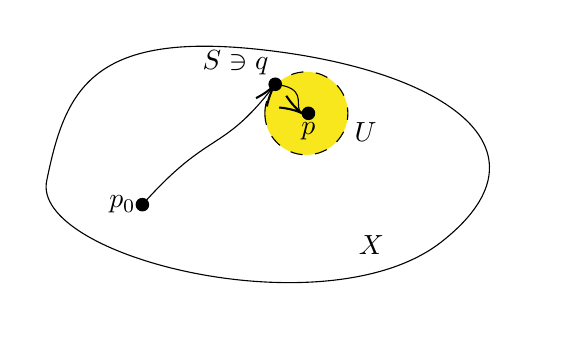
\begin{tikzpicture}[x=0.75pt,y=0.75pt,yscale=-1,xscale=1]
%uncomment if require: \path (0,300); %set diagram left start at 0, and has height of 300

%Curve Lines [id:da5692727890928835] 
\draw    (192,184) .. controls (201,140) and (214,111) .. (301,122) .. controls (388,133) and (437,171) .. (382,214) .. controls (327,257) and (183,221) .. (192,184) -- cycle ;
%Shape: Circle [id:dp048125122285625155] 
\draw  [fill={rgb, 255:red, 248; green, 231; blue, 28 }  ,fill opacity=1 ][dash pattern={on 4.5pt off 4.5pt}] (297,152) .. controls (297,140.95) and (305.95,132) .. (317,132) .. controls (328.05,132) and (337,140.95) .. (337,152) .. controls (337,163.05) and (328.05,172) .. (317,172) .. controls (305.95,172) and (297,163.05) .. (297,152) -- cycle ;
%Curve Lines [id:da8438741294128063] 
\draw    (238,196) .. controls (270.51,159.55) and (275.84,171.62) .. (300.84,139.5) ;
\draw [shift={(302,138)}, rotate = 127.41] [color={rgb, 255:red, 0; green, 0; blue, 0 }  ][line width=0.75]    (10.93,-3.29) .. controls (6.95,-1.4) and (3.31,-0.3) .. (0,0) .. controls (3.31,0.3) and (6.95,1.4) .. (10.93,3.29)   ;
%Shape: Circle [id:dp3225199611789409] 
\draw  [fill={rgb, 255:red, 0; green, 0; blue, 0 }  ,fill opacity=1 ] (315,152) .. controls (315,150.34) and (316.34,149) .. (318,149) .. controls (319.66,149) and (321,150.34) .. (321,152) .. controls (321,153.66) and (319.66,155) .. (318,155) .. controls (316.34,155) and (315,153.66) .. (315,152) -- cycle ;
%Shape: Circle [id:dp19908889775923666] 
\draw  [fill={rgb, 255:red, 0; green, 0; blue, 0 }  ,fill opacity=1 ] (235,196) .. controls (235,194.34) and (236.34,193) .. (238,193) .. controls (239.66,193) and (241,194.34) .. (241,196) .. controls (241,197.66) and (239.66,199) .. (238,199) .. controls (236.34,199) and (235,197.66) .. (235,196) -- cycle ;
%Curve Lines [id:da024774956604691534] 
\draw    (302,138) .. controls (316.79,139.74) and (311.9,146.78) .. (313.67,150.55) ;
\draw [shift={(315,152)}, rotate = 210.96] [color={rgb, 255:red, 0; green, 0; blue, 0 }  ][line width=0.75]    (10.93,-3.29) .. controls (6.95,-1.4) and (3.31,-0.3) .. (0,0) .. controls (3.31,0.3) and (6.95,1.4) .. (10.93,3.29)   ;
%Shape: Circle [id:dp5919265314746458] 
\draw  [fill={rgb, 255:red, 0; green, 0; blue, 0 }  ,fill opacity=1 ] (299,138) .. controls (299,136.34) and (300.34,135) .. (302,135) .. controls (303.66,135) and (305,136.34) .. (305,138) .. controls (305,139.66) and (303.66,141) .. (302,141) .. controls (300.34,141) and (299,139.66) .. (299,138) -- cycle ;

% Text Node
\draw (341,209.4) node [anchor=north west][inner sep=0.75pt]    {$X$};
% Text Node
\draw (236,196) node [anchor=east] [inner sep=0.75pt]    {$p_{0}$};
% Text Node
\draw (300,134.6) node [anchor=south east] [inner sep=0.75pt]    {$S\ni q$};
% Text Node
\draw (339,155.4) node [anchor=north west][inner sep=0.75pt]    {$U$};
% Text Node
\draw (318,155.4) node [anchor=north] [inner sep=0.75pt]    {$p$};


\end{tikzpicture}\caption{命题\ref{c4-m12}中之$S$为闭集}
	\end{figure}
\end{enumerate}
因此$S$是既开又闭集,证毕!
\end{proof}

\chapter{商空间}

%第二部分
\part{代数拓扑}
\chapter{基本群}

%第三部分-流形与几何-梅加强
\part{微分流形}
\chapter{微分流形}

\section{流形的定义与例}

%\chapter{微积分}
%\chapter{流形的几何}
%\chapter{流形的上同调}
%符号说明
\part{杂七杂八}
\chapter{符号说明}
%\begin{mdframed}
%	一切没有符号说明的文档都是耍流氓!
%	
%	\hfill---my帅气的作者\quad
%\end{mdframed}

本讲义有以下符号说明,便于我自己看不明白的时候过来回顾一下(
\section{符号说明}
\begin{enumerate}
	\item $O\subset_{open}X$的含义是$O$是$X$的开子集。
	\item $F\subset_{closed}X$的含义是$F$是$X$的闭子集。
	\item $F=_{closed}X$的含义是$F$和$X$相等,且均为闭集。
	\item 所有的弯体(比如$\subset$)变直之后就表示更加强的区分效果(比如$\sqsubset$,表示真被包含)。
	\item 所有的包含采用类似$\subset$的符号,若出现$\subseteq$(一般不会),表示同一意思。
	\item 同胚的符号主要使用$\cong$,这是因为我想这么用。但是不同胚的符号只能用$\ncong$了,这是因为只有这个符号可以被使用。
	\item 虽然被包含的符号按照流行且不产生歧义的方式使用了$\subset$,但是不被包含的类似符号不存在,因此只好改用$\nsubseteq$。
\end{enumerate}
\section{语法说明}
\begin{enumerate}
	\item 数学逻辑语言同国际标准。
	\item 外加一些张氏古代汉语和标准中式英语(虽然掺杂一些少量标准英式英语)。
\end{enumerate}

\printindex

\end{document}
